% !TeX encoding = UTF-8
% !TeX program = xelatex
% !TeX spellcheck = en_US

\documentclass[degree=bachelor,fontset=windows]{thuthesis}
  % 学位 degree:
  %   doctor | master | bachelor | postdoc
  % 学位类型 degree-type:
  %   academic(默认)| professional
  % 语言 language
  %   chinese(默认)| english
  % 字体库 fontset
  %   windows | mac | fandol | ubuntu
  % 建议终版使用 Windows 平台的字体编译


% 论文基本配置,加载宏包等全局配置
% !TeX root = ./thuthesis-example.tex

% 论文基本信息配置

\thusetup{
  %******************************
  % 注意:
  %   1. 配置里面不要出现空行
  %   2. 不需要的配置信息可以删除
  %   3. 建议先阅读文档中所有关于选项的说明
  %******************************
  %
  % 输出格式
  %   选择打印版(print)或用于提交的电子版(electronic),前者会插入空白页以便直接双面打印
  %
  output = print,
  %
  % 标题
  %   可使用“\\”命令手动控制换行
  %
  title  = {通用稀疏张量计算的编译算法设计},
  title* = {Compilation algorithm design of general sparse tensor algebra},
  %
  % 学位
  %   1. 学术型
  %      - 中文
  %        需注明所属的学科门类,例如:
  %        哲学、经济学、法学、教育学、文学、历史学、理学、工学、农学、医学、
  %        军事学、管理学、艺术学
  %      - 英文
  %        博士:Doctor of Philosophy
  %        硕士:
  %          哲学、文学、历史学、法学、教育学、艺术学门类,公共管理学科
  %          填写“Master of Arts“,其它填写“Master of Science”
  %   2. 专业型
  %      直接填写专业学位的名称,例如:
  %      教育博士、工程硕士等
  %      Doctor of Education, Master of Engineering
  %   3. 本科生不需要填写
  %
  degree-name  = {工学硕士},
  degree-name* = {Master of Science},
  %
  % 培养单位
  %   填写所属院系的全名
  %
  department = {电子工程系},
  %
  % 学科
  %   1. 学术型学位
  %      获得一级学科授权的学科填写一级学科名称,其他填写二级学科名称
  %   2. 工程硕士
  %      工程领域名称
  %   3. 其他专业型学位
  %      不填写此项
  %   4. 本科生填写专业名称,第二学位论文需标注“(第二学位)”
  %
  discipline  = {电子信息科学与技术},
  discipline* = {Electronic Information Science and Technology},
  %
  % 姓名
  %
  author  = {张庚瀚},
  author* = {Zhang Genghan},
  %
  % 指导教师
  %   中文姓名和职称之间以英文逗号“,”分开,下同
  %
  supervisor  = {汪玉, 教授},
  supervisor* = {Professor Wang Yu},
  %
  % 副指导教师
  %
  % associate-supervisor  = {陈文光, 教授},
  % associate-supervisor* = {Professor Chen Wenguang},
  %
  % 联合指导教师
  %
  % co-supervisor  = {某某某, 教授},
  % co-supervisor* = {Professor Mou Moumou},
  %
  % 日期
  %   使用 ISO 格式;默认为当前时间
  %
  % date = {2019-07-07},
  %
  % 是否在中文封面后的空白页生成书脊(默认 false)
  %
  include-spine = false,
  %
  % 密级和年限
  %   秘密, 机密, 绝密
  %
  % secret-level = {秘密},
  % secret-year  = {10},
  %
  % 博士后专有部分
  %
  % clc                = {分类号},
  % udc                = {UDC},
  % id                 = {编号},
  % discipline-level-1 = {计算机科学与技术},  % 流动站(一级学科)名称
  % discipline-level-2 = {系统结构},          % 专业(二级学科)名称
  % start-date         = {2011-07-01},        % 研究工作起始时间
}

% 载入所需的宏包

% 定理类环境宏包
\usepackage{amsthm}
% 也可以使用 ntheorem
% \usepackage[amsmath,thmmarks,hyperref]{ntheorem}

\thusetup{
  %
  % 数学字体
  % math-style = GB,  % GB | ISO | TeX
  math-font  = xits,  % stix | xits | libertinus
}

% 可以使用 nomencl 生成符号和缩略语说明
% \usepackage{nomencl}
% \makenomenclature

% 表格加脚注
\usepackage{threeparttable}

% 表格中支持跨行
\usepackage{multirow}

% 固定宽度的表格。
% \usepackage{tabularx}

% 跨页表格
\usepackage{longtable}

% 算法
\usepackage{algorithm}
\usepackage{algorithmic}

% 量和单位
\usepackage{siunitx}

% 参考文献使用 BibTeX + natbib 宏包
% 顺序编码制
\usepackage[sort]{natbib}
\bibliographystyle{thuthesis-numeric}

% 著者-出版年制
% \usepackage{natbib}
% \bibliographystyle{thuthesis-author-year}

% 本科生参考文献的著录格式
% \usepackage[sort]{natbib}
% \bibliographystyle{thuthesis-bachelor}

% 参考文献使用 BibLaTeX 宏包
% \usepackage[style=thuthesis-numeric]{biblatex}
% \usepackage[style=thuthesis-author-year]{biblatex}
% \usepackage[style=apa]{biblatex}
% \usepackage[style=mla-new]{biblatex}
% 声明 BibLaTeX 的数据库
% \addbibresource{ref/refs.bib}

% 定义所有的图片文件在 figures 子目录下
\graphicspath{{figures/}}

% 数学命令
\makeatletter
\newcommand\dif{%  % 微分符号
  \mathop{}\!%
  \ifthu@math@style@TeX
    d%
  \else
    \mathrm{d}%
  \fi
}
\makeatother

% hyperref 宏包在最后调用
\usepackage{hyperref}



\begin{document}

% 封面
\maketitle

% 使用授权的说明
% \copyrightpage
% 将签字扫描后授权文件 scan-copyright.pdf 替换原始页面
% \copyrightpage[file=scan-copyright.pdf]

\frontmatter
% !TeX root = ../thuthesis-example.tex

% 中英文摘要和关键字

\begin{abstract}
  本文针对单指令多线程架构上的稀疏稠密混合代数算子,提出了新的优化技术并设计了相应的编译算法,使得算子性能和开发效率两方面都取得了提升,并为更广泛的通用稀疏张量计算编译算法设计提出了可行的研究方法。
  
  稀疏张量是指大部分元素为零的张量。稀疏稠密混合代数指作用在一个稀疏张量和至少一个稠密张量上的张量代数。该种代数被广泛应用在图神经网络,稀疏神经网络,数据分析和高性能计算中。
  但稀疏稠密混合代数在单指令多线程架构上优化仍不充分,而且开发难度较高。

  针对这两个问题,本文提出了灵活规约优化技术和灵活规约语义提升技术。
  灵活规约优化技术包含灵活规约粒度和规约策略,该技术扩展了当前的稀疏稠密混合代数优化空间,同时在原理上可以将性能提升泛化至所有稀疏稠密混合代数。在稀疏稠密矩阵向量乘算子上灵活规约取得了比最优开源算子库平均1.6到2.7倍性能提升。
  基于扩展后的优化空间,本文将灵活规约纳入稀疏迭代模型,并提出灵活规约语义提升技术。该技术使得用户可以通过简单调度指令针对任意稀疏稠密混合代数进行性能调优。运用该技术后,稀疏算子编译器生成的二维稀疏稠密矩阵向量乘算子性能平均提升1.2倍,最多提升3.8倍;三维矩阵化张量乘Khatri-Rao积算子最高提升2.7倍。
  
  % 关键词用“英文逗号”分隔,输出时会自动处理为正确的分隔符
  \thusetup{
    keywords = {稀疏张量代数, 编译器, 高性能算子, 单指令多线程架构},
  }
\end{abstract}

\begin{abstract*}
  This paper proposes flexible reduction to expand the optimization space of sparse-dense hybrid algebra kernels on SIMT architecture.
  Furthermore, it proposes a compilation algorithm to utilize flexible reduction in sparse compilers. These techniques improve the performance of 
  sparse-dense hybrid algebra kernels and the efficiency of development and performance tuning. This paper concludes the optimization technique from specific kernels, then generalizes it to other kernels, and finally designs 
  a compilation algorithm to tune kernel performance efficiently. Such research method can be generalized to the compilation algorithm design for general sparse tensor algebra.

  Sparse tensors are tensors whose elements are mostly zero. Sparse-dense hybrid algebra exerts on a sparse tensor and at least one dense tensor. 
  Sparse-dense hybrid algebra is widely used in graph neural networks, sparse neural networks, data analysis, and high-performance computing. 
  However, the optimization of such algebra on SIMT architecture is still insufficient, and the generalization and performance tuning cost is too high.

  To solve these two challenges, this paper proposes flexible reduction optimization and compilation algorithm. Flexible reduction is composed of flexible granularity and flexible strategy. 
  This technique expands the optimization space of sparse dense hybrid tensor algebra, and in theory is applicable to any sparse dense hybrid tensor algebra. It improves the performance
  of the state-of-the-art SpMM library by $1.6x \sim 2.7x$ on average. Based on the expanded optimization space, this paper includes flexible reduction to the sparse iteration model and proposes the semantic elevation technique.
  Such a technique enables users to tune the performance of flexible reduction on any sparse-dense hybrid algebra using simple schedule language. Equipped with this technique, the sparse compiler can generate SpMM kernels up to 3.8x (1.2x on average) faster and MTTKRP kernels up to 2.7 times faster.
  % Use comma as separator when inputting
  \thusetup{
    keywords* = {Sparse tensor algebra, Compiler, High performance kernel, SIMT},
  }
\end{abstract*}


% 目录
\tableofcontents

% 插图和附表清单
% 本科生的插图索引和表格索引需要移至正文之后、参考文献前
% \listoffiguresandtables  % 插图和附表清单(仅限研究生)


% 符号对照表
% !TeX root = ../thuthesis-example.tex

\begin{denotation}[3cm]
  \item[SpMM] 稀疏稠密矩阵乘法
  \item[SDDMM] 采样稠密矩阵乘法 
  \item[MTTKRP] 矩阵化张量乘Khatri-Rao积 
  \item[TTM] 张量矩阵乘法
  \item[N] 稀疏稠密矩阵乘法中稠密矩阵列数
  \item[TF] 张量形式的稀疏稠密混合代数
  \item[DF] 表形式的稀疏稠密混合代数  
  \item[$\symbf{Y}$] 稠密输出张量  
  \item[$\symbf{A}$] 稀疏输入张量  
  \item[$\symbf{X}$] 稠密输入张量
  \item[$Q$] 张量对应的表 
  \item[CIN] 具象角标表示
  \item[LLIR] 低层次中间表示   
  \item[SIMT] 单指令多线程 
\end{denotation}



% 也可以使用 nomencl 宏包,需要在导言区
% \usepackage{nomencl}
% \makenomenclature

% 在这里输出符号说明
% \printnomenclature[3cm]

% 在正文中的任意为都可以标题
% \nomenclature{PI}{聚酰亚胺}
% \nomenclature{MPI}{聚酰亚胺模型化合物,N-苯基邻苯酰亚胺}
% \nomenclature{PBI}{聚苯并咪唑}
% \nomenclature{MPBI}{聚苯并咪唑模型化合物,N-苯基苯并咪唑}
% \nomenclature{PY}{聚吡咙}
% \nomenclature{PMDA-BDA}{均苯四酸二酐与联苯四胺合成的聚吡咙薄膜}
% \nomenclature{MPY}{聚吡咙模型化合物}
% \nomenclature{As-PPT}{聚苯基不对称三嗪}
% \nomenclature{MAsPPT}{聚苯基不对称三嗪单模型化合物,3,5,6-三苯基-1,2,4-三嗪}
% \nomenclature{DMAsPPT}{聚苯基不对称三嗪双模型化合物(水解实验模型化合物)}
% \nomenclature{S-PPT}{聚苯基对称三嗪}
% \nomenclature{MSPPT}{聚苯基对称三嗪模型化合物,2,4,6-三苯基-1,3,5-三嗪}
% \nomenclature{PPQ}{聚苯基喹噁啉}
% \nomenclature{MPPQ}{聚苯基喹噁啉模型化合物,3,4-二苯基苯并二嗪}
% \nomenclature{HMPI}{聚酰亚胺模型化合物的质子化产物}
% \nomenclature{HMPY}{聚吡咙模型化合物的质子化产物}
% \nomenclature{HMPBI}{聚苯并咪唑模型化合物的质子化产物}
% \nomenclature{HMAsPPT}{聚苯基不对称三嗪模型化合物的质子化产物}
% \nomenclature{HMSPPT}{聚苯基对称三嗪模型化合物的质子化产物}
% \nomenclature{HMPPQ}{聚苯基喹噁啉模型化合物的质子化产物}
% \nomenclature{PDT}{热分解温度}
% \nomenclature{HPLC}{高效液相色谱(High Performance Liquid Chromatography)}
% \nomenclature{HPCE}{高效毛细管电泳色谱(High Performance Capillary lectrophoresis)}
% \nomenclature{LC-MS}{液相色谱-质谱联用(Liquid chromatography-Mass Spectrum)}
% \nomenclature{TIC}{总离子浓度(Total Ion Content)}
% \nomenclature{\textit{ab initio}}{基于第一原理的量子化学计算方法,常称从头算法}
% \nomenclature{DFT}{密度泛函理论(Density Functional Theory)}
% \nomenclature{$E_a$}{化学反应的活化能(Activation Energy)}
% \nomenclature{ZPE}{零点振动能(Zero Vibration Energy)}
% \nomenclature{PES}{势能面(Potential Energy Surface)}
% \nomenclature{TS}{过渡态(Transition State)}
% \nomenclature{TST}{过渡态理论(Transition State Theory)}
% \nomenclature{$\increment G^\neq$}{活化自由能(Activation Free Energy)}
% \nomenclature{$\kappa$}{传输系数(Transmission Coefficient)}
% \nomenclature{IRC}{内禀反应坐标(Intrinsic Reaction Coordinates)}
% \nomenclature{$\nu_i$}{虚频(Imaginary Frequency)}
% \nomenclature{ONIOM}{分层算法(Our own N-layered Integrated molecular Orbital and molecular Mechanics)}
% \nomenclature{SCF}{自洽场(Self-Consistent Field)}
% \nomenclature{SCRF}{自洽反应场(Self-Consistent Reaction Field)}



% 正文部分
\mainmatter
% !TeX root = ../thuthesis-example.tex

\chapter{引言}

\section{研究问题}
张量可以被用于描述事物之间的线性关系,张量代数则是作用在张量上,对张量所表示关系进行分析的数学工具。
比如在线性系统中,使用二维张量(矩阵)表示系统状态,用矩阵变换表示系统与环境的交互。如果把张量的每个维度看做一种数据,那么张量就可以表示
这些不同种数据之间的关系。比如,在图~\ref{fig:intro}中,利用矩阵乘法即可完成作者引用文章的分析。相似的,社交网络中不同群体的关系,金融计算中不同
交易主体之间的交易信息等,都可以利用张量表示并利用张量代数进行分析。
\begin{figure}
  \centering
  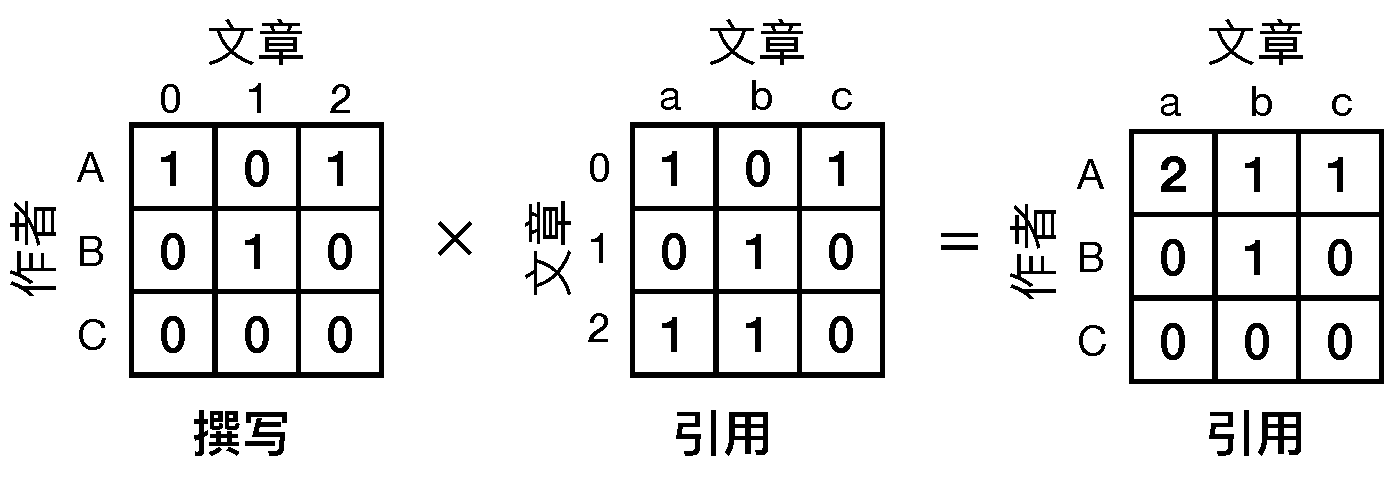
\includegraphics[width=0.9\linewidth]{intro.pdf}
  \caption{稀疏张量代数示例}
  \caption*{第一个矩阵的第一维表示作者,第二维表示文章,矩阵表示的关系是作者写文章。第二个矩阵的第一维表示文章,第二维表示文章,矩阵表示的关系是文章引用文章。
  两个矩阵做矩阵乘法运算后得到的矩阵第一维表示作者,第二维表示文章,关系则变为作者引用文章。}
  \label{fig:intro}
\end{figure}

在现实应用中,因为稀疏关系是普遍存在的\cite{uzzi2007small},所以张量通常是稀疏的。比如在深度神经网络中,不同神经元间连接是稀疏的,体现在权重张量上就是其大部分($50\% \sim 90\%$)可以是零\cite{wang2021dual}。
再比如以及记录亚马逊网站截至2013年3月的横跨18年的用户数据的三维张量中,每一个非零元素对应近80亿个零元\cite{mcauley2013hidden}。
随着稀疏性在神经网络的广泛应用\cite{xiao2022smoothquant},以及现实生活中关系数据的日益增长,需要研究更高效的稀疏张量运算。

然而,稀疏计算优化在算子优化技术和算法开发成本上仍面临挑战。一方面,由于稀疏计算的不规则性,在当前主流并行计算平台上的高效算法的研究仍不充分。另一方面,由于稀疏计算在代数表达和优化技巧方面的多样性,当前稀疏算子库模式开发成本过高。

虽然GPU提供了10TFLOP/s量级的并行计算能力,但是由于稀疏张量计算的不规则性,充分利用GPU的并行计算能力仍具有挑战性。表\ref{tab:motivation-1}展示了SDDMM\cite{yu2021exploiting},SpMM\cite{huang2020ge},MTTKRP\cite{nisa2019mttkrp},其中每种算子均采用当前性能最高的开源库。
\begin{table}
  \centering
  \caption{稀疏张量算子库性能和GPU峰值算力对比}
  \begin{tabular}{llll}
    \toprule
    算子名  & 算子性能(TFLOP/s) & 平台峰值算力(TFLOP/s) & 与峰值算力差距倍数   \\
    \midrule
    SDDMM  & 0.42 & 15.7 & 37.4x \\
    SpMM   & 0.28 & 10.6 & 37.9x \\
    MTTKRP & 0.20 & 15.7 & 78.5x \\
    \bottomrule
  \end{tabular}
  \label{tab:motivation-1}
\end{table}
从表\ref{tab:motivation-1}中可以看出,最佳的开源稀疏张量算子库算子性能和平台峰值算力还有几十倍的差距,这说明计算平台的算力还没有被充分利用。因此主要挑战是如何进一步扩展优化空间,即写出更高效的稀疏张量算子。

除了算子性能较低,现在编写高性能稀疏算子库也较为困难。这里用代码行数来衡量编写算子库的难易程度。表\ref{tab:motivation-2}展示了SDDMM,SpMM,MTTKRP最佳算子库和稀疏张量编译器TACO的对比。其中算子库代码行数指编写GPU上执行的CUDA算子需要的代码行数(不包括CPU和GPU间数据搬移和算子调用的代码),算子编译器代码行数指运用TACO提供的调度变换指令编写算子所需要的代码行数。
\begin{table}
  \centering
  \begin{threeparttable}[c]
  \caption{稀疏张量算子库和算子编译器的性能和代码行数对比}
  \label{tab:motivation-2}
  \begin{tabular}{lllll}
    \toprule
    算子名  & 算子库 & 算子编译器 & 算子库与编译器 & 算子库与编译器   \\
           & 代码行数 & 代码行数 & 代码行数比    & 算子性能比       \\
    \midrule
    SDDMM\tnote{a}  & 53 & 12 & 4.4x & 2.1x \\
    SpMM\tnote{b}   & 132 & 13 & 10.2x & 2.6x \\
    MTTKRP\tnote{c} & 40 & 12 & 3.3x & 1.2x \\
    \bottomrule
  \end{tabular}
  \begin{tablenotes}
    \item [a] 选取SOTA的GPU开源SDDMM算子库 PRedS \cite{yu2021exploiting}中的sddmm\_csr\_ebalance\_vec4函数和TACO中的scheduleSDDMMGPU函数做对比。
    \item [b] 选取SOTA的GPU开源SpMM算子库 DASpMM \cite{dai2022heuristic}中的采用的四种算子:csrspmm\_rowcaching\_rowbalance\_kernel,
      csrspmm\_rowcaching\_nnzbalance\_kernel,csrspmm\_parreduce\_rowbalance\_kernel和csrspmm\_parreduce\_nnzbalance\_kernel函数的平均行数和TACO中的scheduleSpMMGPU函数对比。
    \item [c] 选取SOTA的GPU开源MTTKRP算子库MM-CSF\cite{nisa2019mttkrp}中采用HyB格式的3维MTTKRP函数的平均行数和TACO中的scheduleMTTKRPGPU函数对比。
  \end{tablenotes}
  \end{threeparttable}
\end{table}
从表\ref{tab:motivation-2}中可以看出,利用编译器提供的领域专用语言可以减小3到10倍的代码量,但是会牺牲16\%到60\%的性能。性能下降说明编译器表达的优化空间没有包含已有算子库的优化技巧。
因此,需要设计更好的编译算法,在进一步降低用户代码量的同时,扩展优化空间,从而使得用户可以用更低的开发难度得到更高性能的稀疏张量算子。

\section{本文贡献}
本文针对算子性能低的问题提出新的算子优化技术,并针对优化技巧在不同稀疏张量运算的迁移问题提出更高效的稀疏编译算法,在提升算子性能同时降低部署复杂度。

本文提出了灵活规约优化技术,这是一种新的针对SIMT架构上稀疏稠密混合张量代数算子优化技术。该技术扩展了优化空间,进一步提升了算子库性能。实验表明,采用灵活规约同步后可以将SpMM算子库性能提升平均1.6至2.3倍(针对不同代GPU架构加速比有所不同)。

基于灵活规约优化技术,本文提出了灵活规约语义提升技术,这是一种新的针对SIMT架构上稀疏稠密混合张量代数的编译算法。该技术扩展了稀疏算子编译器表达的优化空间,同时在用户端只需要增加一行代码即可获得灵活规约带来的算子加速。
实验表明,采用该技术后,编译器生成SpMM算子性能提升了平均1.2倍,最多提升3.8倍;编译器生成MTTKRP算子性能最多提升2.7倍。

\section{本文框架}
本文第2章介绍了稀疏稠密混合代数,针对GPU上稀疏稠密混合代数的优化技术,以及稀疏算子编译器的背景知识和相关工作。第3章阐释了灵活规约的内涵,构建了基于灵活规约的
扩展优化空间,并通过实验验证了灵活规约的有效性,探讨了优化空间的结构。第4章阐述了灵活规约语义提升技术的定义,介绍了算法流程和系统部署,并通过实验验证了编译算法针对稀疏稠密混合代数优化的有效性。第5章总结了本文的工作,
并为未来算子编译器研究提出可能的研究问题。

% !TeX root = ../thuthesis-example.tex

\chapter{背景介绍}

\section{稀疏张量代数}
稀疏张量代数(Sparse Tensor Algebra)是指作用在存在大量零元的张量上的张量代数。与稠密张量代数不同,因为稀疏张量中仅有少量非零元,所以一般按照压缩格式存储,比如DCSR\cite{DCSR},CSB\cite{CSB},DIA\cite{DIA},CSF\cite{CSF}等。
稀疏张量代数有广泛应用。比如在机器学习中,图神经网络\cite{kipf2016semi, hamilton2017inductive}中核心算子为稀疏稠密矩阵乘法和采样稠密矩阵乘法,稀疏卷积神经网络中权重、激活等剪枝后也会出现稀疏张量运算\cite{liu2015sparse}。
在数据分析和高性能计算中,会运用稀疏张量低秩分解\cite{kolda2009tensor}和稀疏矩阵稠密向量乘法\cite{bell2012exposing}等稀疏张量代数。图~\ref{fig:sparse-intro}展示了稀疏矩阵的例子,以及两种压缩存储格式。
CSR格式由三个数组组成,行范围数组中第$i+1$个元素和第$i$个元素的差值代表第$i$行中非零元个数,列序号数组中第$i$个元素代表第$i$个非零元的列序号,非零值数组中第$i$个元素代表第$i$个非零元的值。
COO格式由三个数组组成,行序号数组中第$i$个元素代表第$i$个非零元的行序号,列序号数组中第$i$个元素代表第$i$个非零元的列序号,非零值数组中第$i$个元素代表第$i$个非零元的值。
\begin{figure}
  \centering
  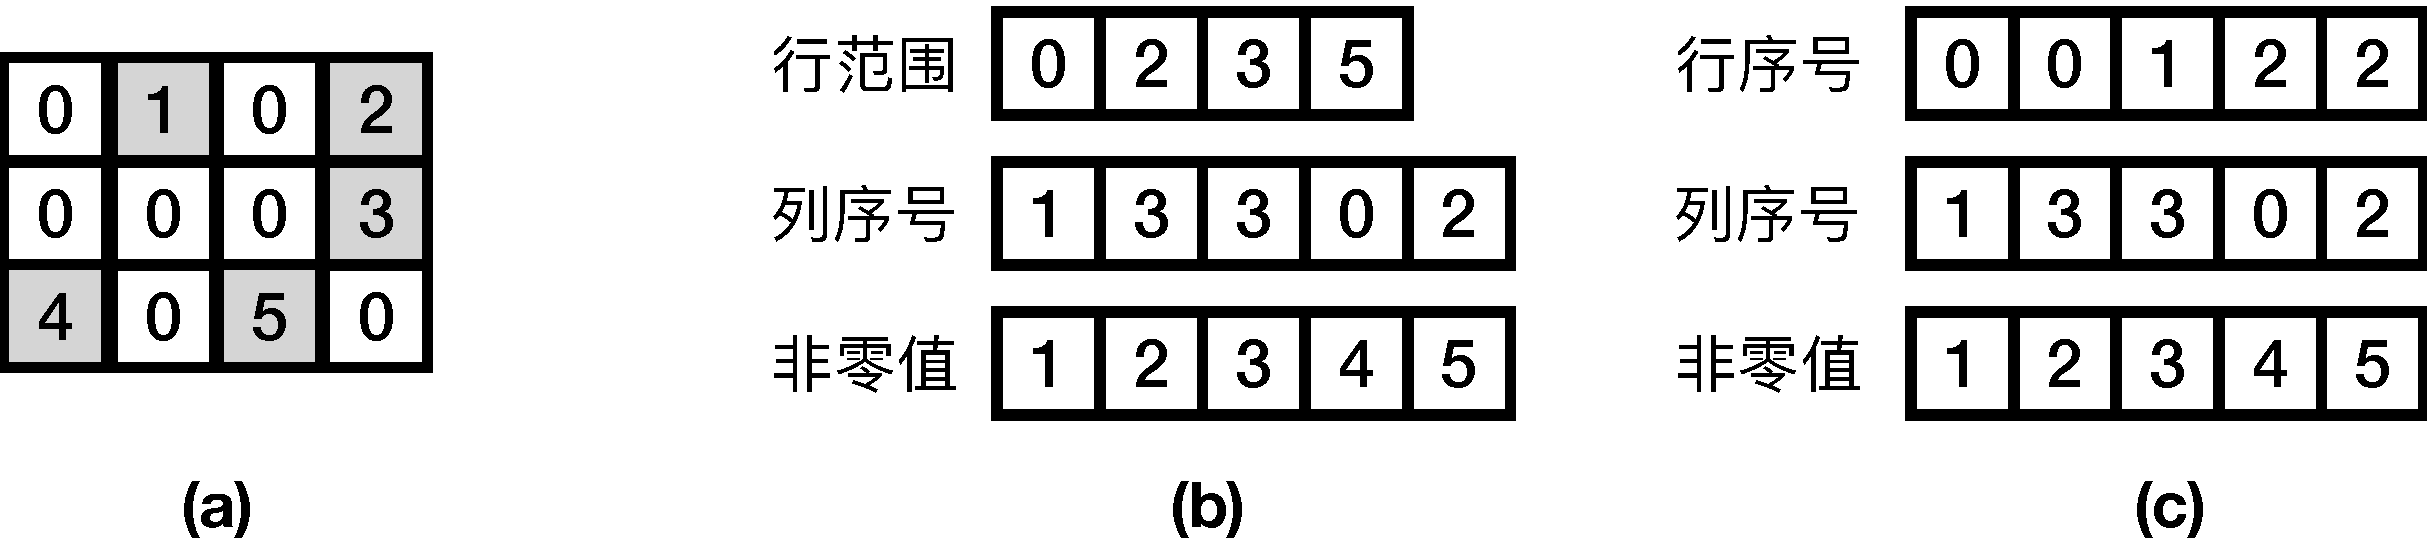
\includegraphics[width=0.99\linewidth]{稀疏矩阵示意图.pdf}
  \caption*{(a)稀疏矩阵;(b)稀疏矩阵压缩稀疏行(CSR)存储格式;(c)稀疏矩阵压缩坐标(COO)存储格式}
  \caption{稀疏矩阵示例}
  \label{fig:sparse-intro}
\end{figure}

\section{稀疏稠密混合代数}
\subsection{定义}
稀疏稠密混合代数是一种稀疏张量代数,它有两种等价的表示形式:一种是张量形式(Tensor formulation,简称TF)如公式\eqref{eq:algebra-view}所示,另一种是表形式(Database formulation,简称DF)如公式\eqref{eq:db-view}所示~\cite{zhang2023sgap}。
在公式\eqref{eq:algebra-view}中,$\symbf{Y}$是输出张量,$\symbf{X^j}$是稠密输入张量,$\symbf{A}$是稀疏输入张量。$\symbf{A}$是稀疏的意味着至少有一个维度$a_i$是以压缩格式存储的。$y_1, y_2,\cdots,y_M$,$a_1, a_2,\cdots,a_N$,$x_1^j,x_2^j,\cdots,x_{M^j}^j$是属于相同的下标变量集合。$M$是输出张量的维度,$N$是输入稀疏张量的维度,$D$是输入稠密张量的个数,$M^j$是输入稠密张量$\symbf{X^j}$的维度。
在公式\eqref{eq:db-view}中本文使用信息传播描述描述稀疏稠密混合代数。$Q,Q_0,Q_1,Q_2$是向关联表的查询。
本文遵循经典的逻辑-物理分离存储思想\cite{codd1970relational}。$D$是$Q$的关联表,
按照$id$升序存储$(id, value)$,其中$id\in \mathbb{Z}$,$value \in \mathbb{R}^n$。$dst\in K$是任何可以哈希的键值,$f$是$K\rightarrow \mathbb{Z}$的映射。
$Q(k)$的值定义为$Q(dst)=D(f(dst))$。$\oplus$可以是任何满足交换律的算符,$\otimes$可以是任何可以接受两个对象作为输入,输出一个可被$\oplus$运算的对象。
$\oplus$的结果会被写入$Q$中的$f(dst)$位置。在DF视角下,稀疏稠密混合代数的稀疏性体现在对于所有$dst$,$Q_0(dst)$是分散的。换句话说,$Q_0(i) \bigcap Q_0(i+1) \sim \emptyset $。
该代数的稠密性体现在$D,D_1,D_2$中的值可以是标量,稠密向量或稠密矩阵。
\begin{equation}
  \symbf{Y}_{y_1, y_2,\cdots,y_M} = \symbf{A}_{a_1, a_2,\cdots,a_N}\prod_{i=1}^{D}\symbf{X}^{j}_{x_1^j,x_2^j,\cdot,x_{M^j}^j}
  \label{eq:algebra-view}
\end{equation}
\begin{equation}
  Q(dst)=\oplus_{src\in Q_0(dst)}\{src, \otimes(Q_1(src,dst), Q_2(dst))\}
  \label{eq:db-view}
\end{equation}
在TF下,稀疏稠密混合代数特征是输入既有稀疏又有稠密张量。在TF下,张量矩阵乘TTM(Tensor Times Matrix Product)\cite{kurt2022ttm},MTTKRP,SDDMM和SpMM四类算子可以表示为公式\eqref{eq:four-expressions}
\begin{subequations}
  \begin{equation}
      \symbf{Y}_{i,j} = \symbf{A}_{i,k,l}\symbf{X}_{k,j}^1\symbf{X}_{l,j}^2
  \end{equation}
  \begin{equation}
      \symbf{Y}_{i,j,l} = \symbf{A}_{i,j,k}\symbf{X}_{k,l}^1
  \end{equation}
  \begin{equation}
      \symbf{Y}_{i,k} = \symbf{A}_{i,k}\symbf{X}_{i,j}^1\symbf{X}_{j,k}^2
  \end{equation}
  \begin{equation}
      \symbf{Y}_{i,k} = \symbf{A}_{i,j}\symbf{X}_{j,k}^1
  \end{equation}
  \label{eq:four-expressions}
\end{subequations}
\subsection{规约}\label{sec:reduction-core}
规约是指在一个基于压缩格式的稀疏向量和一个稠密向量间做向量内积。稀疏稠密混合代数的核心操作是规约。这一个核心观察启发本文针对规约做优化,因为本文只需要加速这一个核心操作,然后通过编译器技术来自动加速不同的稀疏稠密混合代数。
例如在TF视角下,公式\eqref{eq:algebra-view}算子在MTTKRP的$l,k$维度做规约,TTM在$k$维度,SDDMM在$j$维度,SpMM在$j$维度做规约。规约可以在一个稀疏和一个稠密维度之间进行,比如MTTKRP,TTM和SpMM。
规约也可以在两个稠密维度做,比如SDDMM。图~\ref{fig:kernels}展示了这四种算子的规约维度。本文也在图~\ref{fig:four-code}中给出了规约的具体代码例子。例如,MTTKRP包含两个规约,每个规约都和SpMM中的
规约动作一致。这样的性质也可以在DF视角下观察到。 如图~\ref{fig:redb-spmm}和图~\ref{fig:redb-mttkrp},对于MTTKRP和SpMM的第一个规约,$D_1$的值都是标量,$D_2$的值都是向量。对于MTTKRP的第二个规约,尽管$D_1$的值是一个向量,这一点和SpMM不同,
但是$\oplus$行为一致,因为$\otimes$执行的是向量的逐元素乘法。
\begin{figure}[h]%
  \centering
  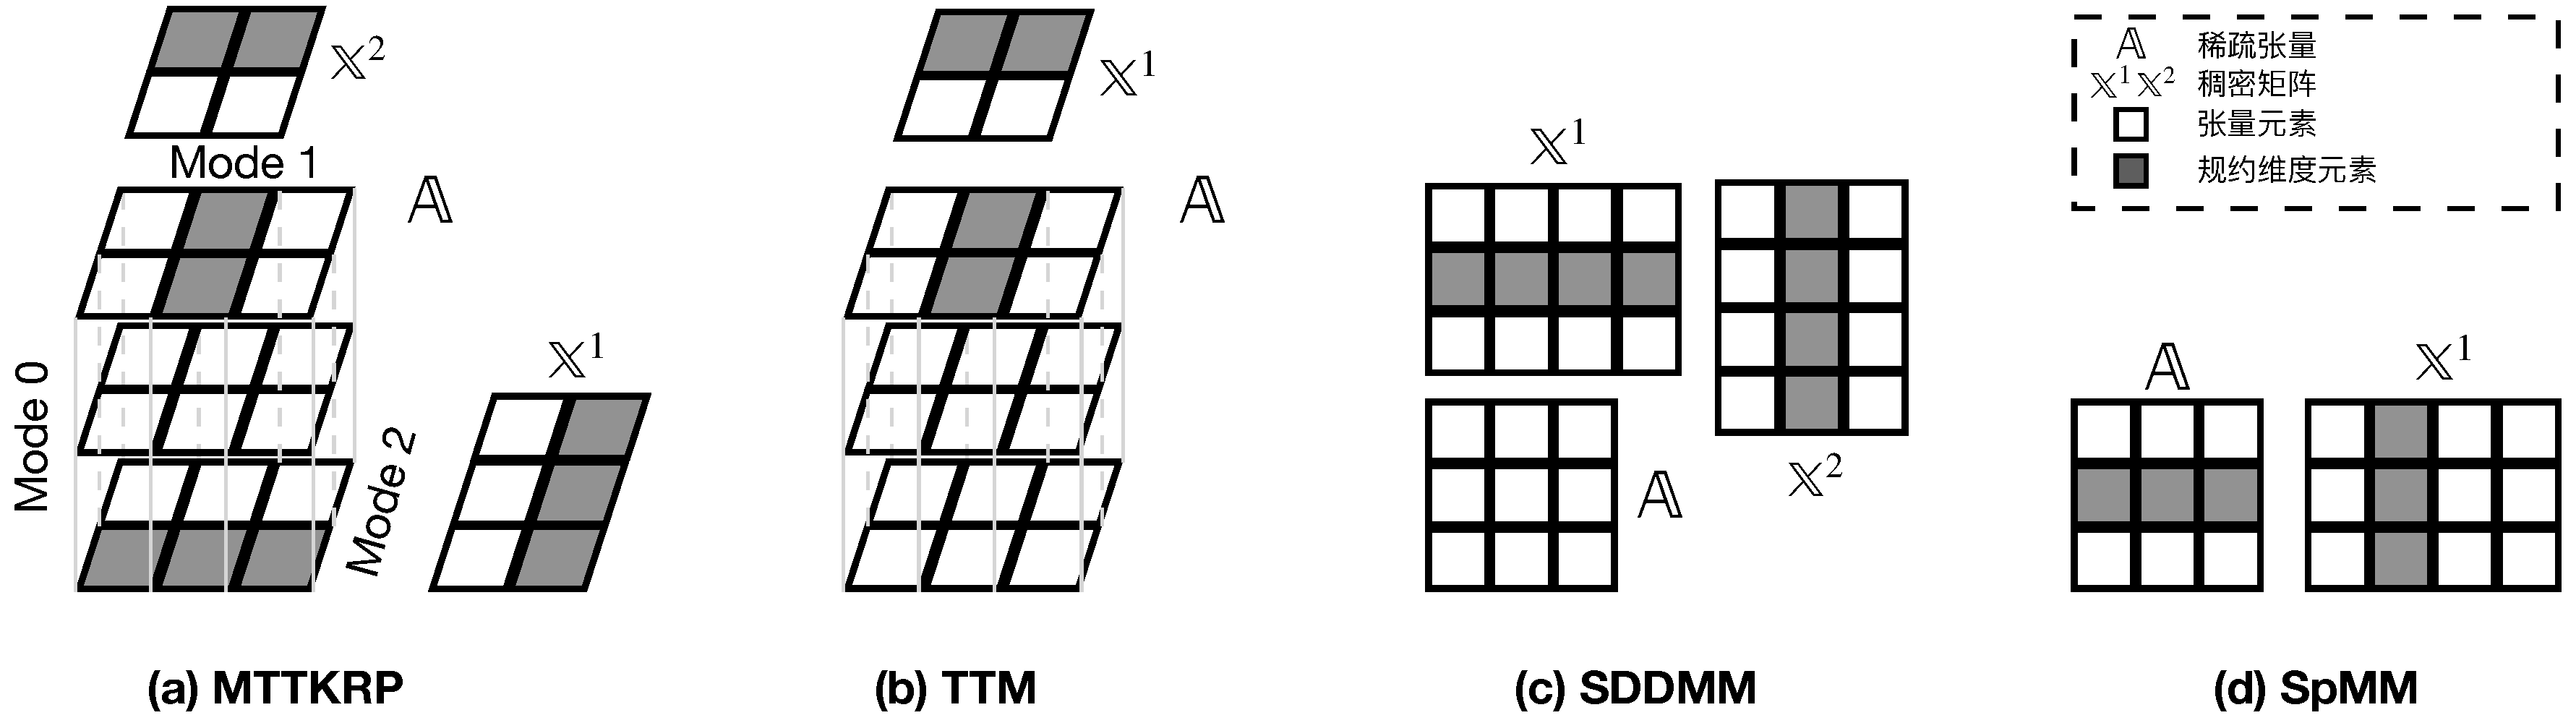
\includegraphics[width=0.99\textwidth]{kernels-cn.pdf}
  \caption{TF视角下稀疏稠密混合代数示例}
  \label{fig:kernels}
\end{figure}
\begin{figure}[h]%
  \centering
  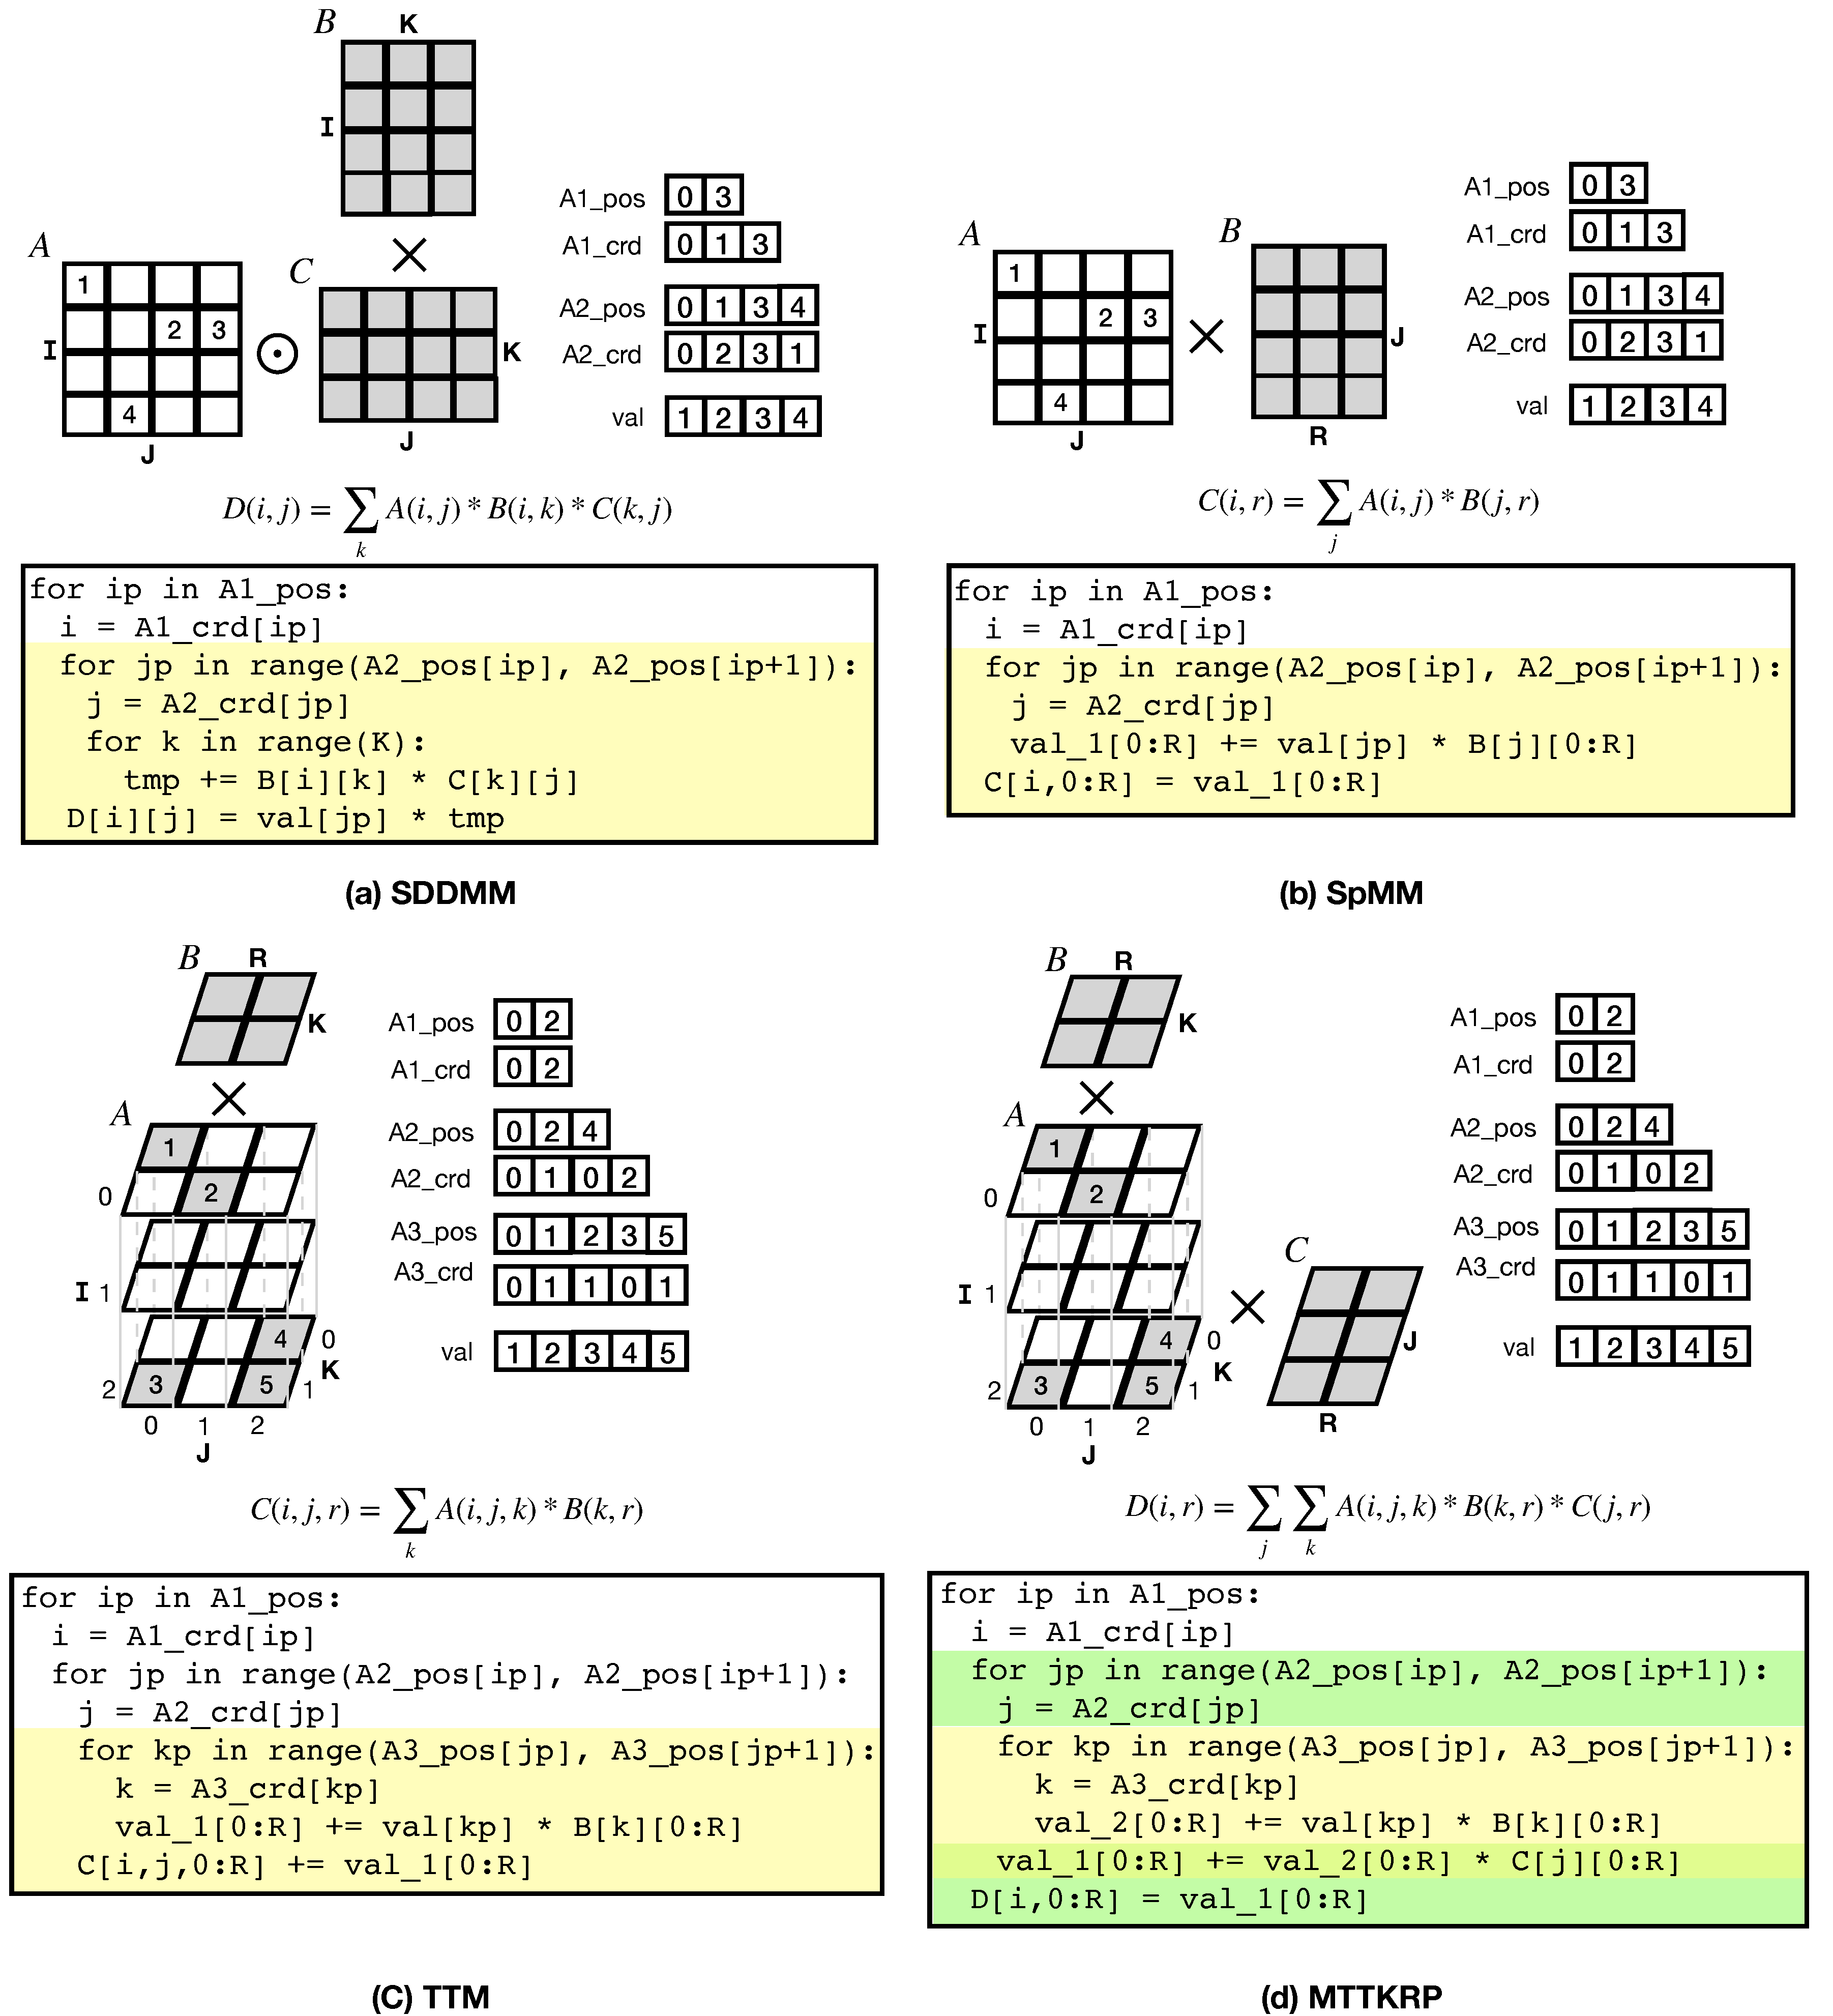
\includegraphics[width=0.99\textwidth]{SpHY.pdf}
  \caption*{黄色的和绿色的代码行是规约代码。MTTKRP有两个层次的规约,分别用黄色和绿色表示。重叠部分代表第一个层级的规约输出是第二个层级规约的输入。对于A的压缩存储本文遵循\cite{kjolstad:2020:phd-thesis}的命名规则。}
  \caption{TF视角下稀疏稠密混合代数规约的代码示例}
  \label{fig:four-code}
\end{figure}
\begin{figure}[h]%
  \centering
  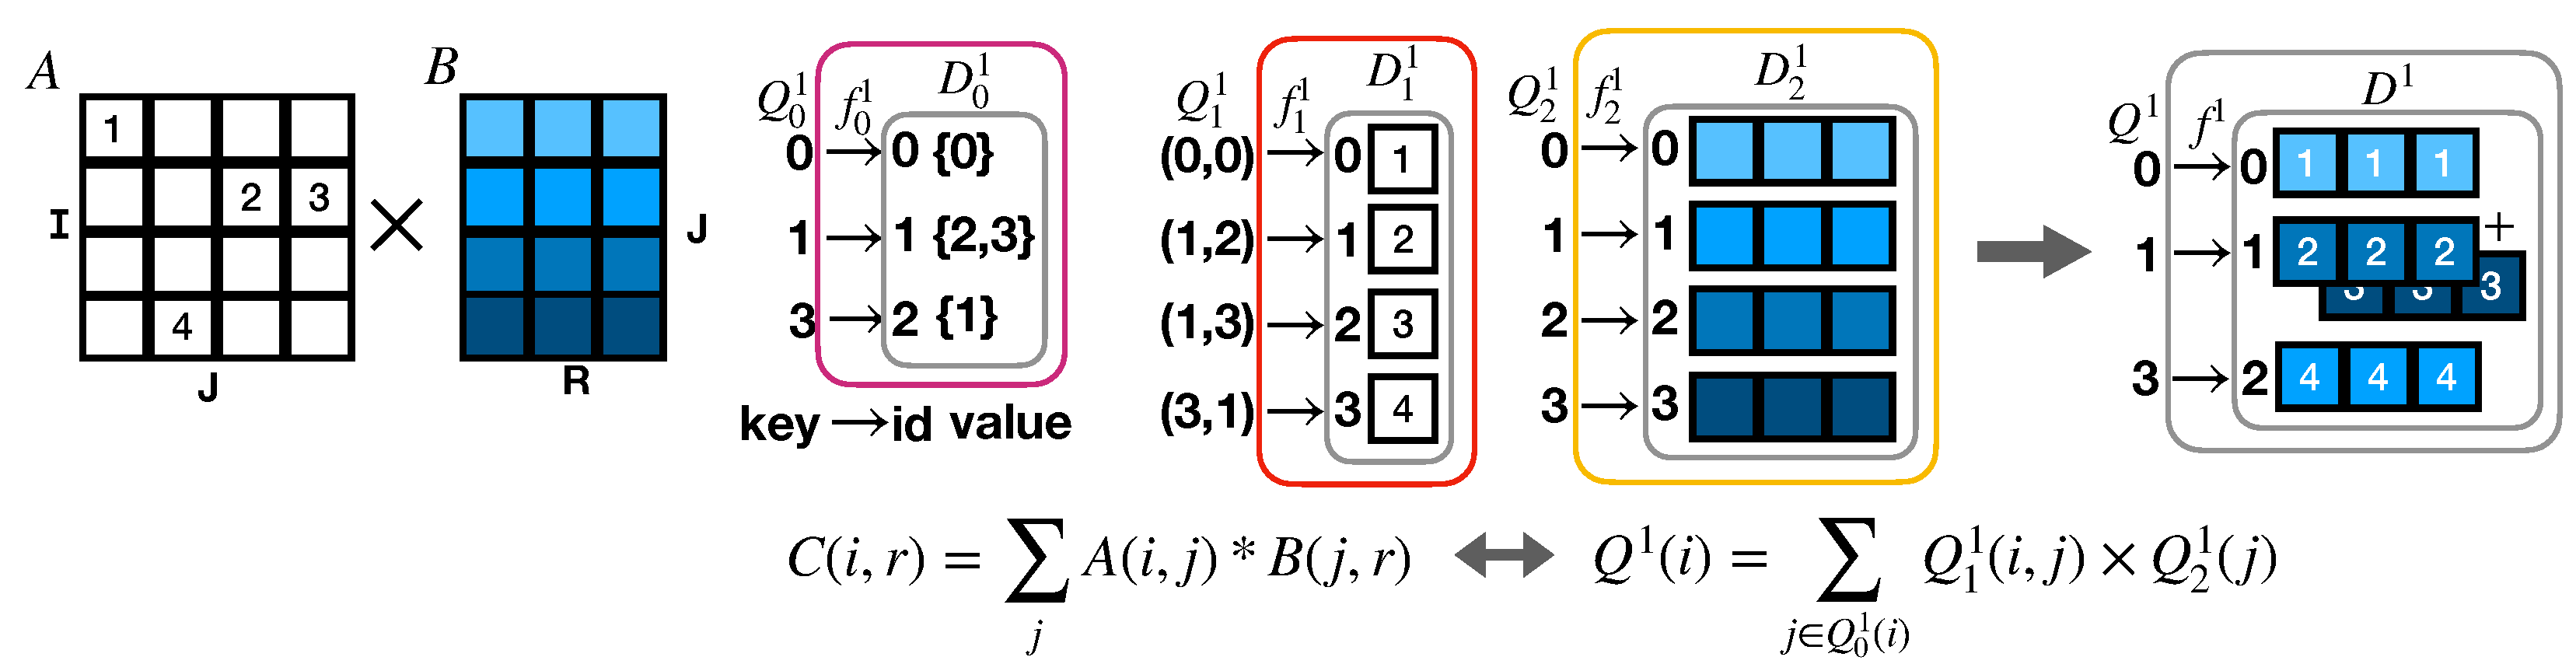
\includegraphics[width=0.99\textwidth]{reduction-db-spmm.pdf}
  \caption{SpMM规约操作示意图}
  \caption*{图片下方展示了该算子在TF和DF视角下等效的表达}
  \label{fig:redb-spmm}
\end{figure}
\begin{figure}[h]%
  \centering
  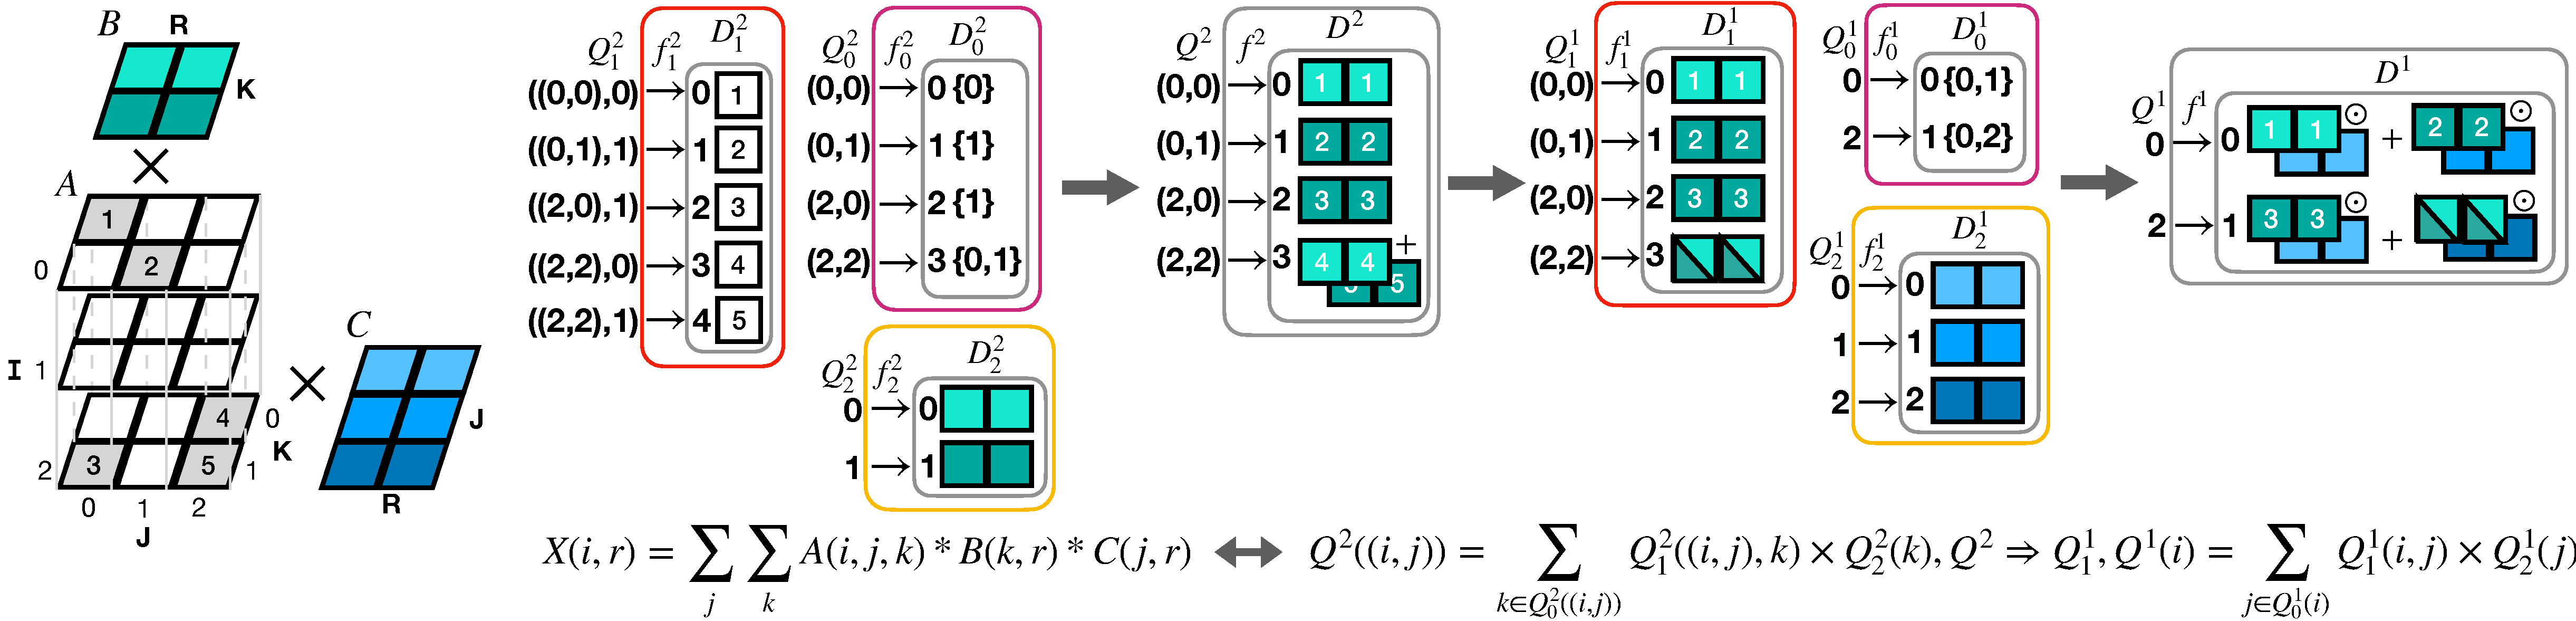
\includegraphics[width=0.99\textwidth]{reduction-db-mttkrp.pdf}
  \caption{MTTKRP规约操作示意图}
  \caption*{图片下方展示了该算子在TF和DF视角下等效的表达}
  \label{fig:redb-mttkrp}
\end{figure}
\section{研究现状}
\subsection{稀疏稠密张量代数GPU优化技术}\label{sec:spmmopt}
如上节所述,规约是稀疏稠密混合张量代数的核心操作,不同算子之间会共享同类型的规约。因此,不失一般性,本文介绍SpMM在GPU上的算子优化技术。
这些优化技术经过简单扩展就可以应用到其他的稀疏稠密混合代数算子中。Yang等人\cite{yang2018design}通过动态选择两个算法来实现在不同并行处理器中非零元个数的平均分配,和不同线程之间的行平均分配。自适应稀疏切分(ASpT)\cite{hong2019adaptive}通过非零元位置重排实现更好的数据局部性,因此降低了向全局内存的访问次数。
Ge-SpMM\cite{huang2020ge}提出了协调行快取技术(Coalesced Row Caching)来实现向稀疏和稠密矩阵的协调内存访问。同时提出了粗粒度线程组合并技术(Coarse-grained Warp Merging)去合并SpMM在不同线程组的工作负载,并实现更好的稀疏矩阵数据复用。Mehrabi等人\cite{mehrabi2021learning}提出了针对CSR格式的行交换技术来实现更好的工作负载均衡和数据局部性。
DA-SpMM\cite{dai2022heuristic}提出了SpMM的三个设计维度,分别是行/非零元均衡、行/列起始循环,并行/串行规约,并基于机器学习算法设计了自动算子选择器。

\subsection{稀疏算子编译器}\label{sec:spcomp}
优化稀疏张量代数有四个维度的复杂度:数据格式、代数表达、优化技巧和硬件平台。如前所述,常见数据格式有CSR,CSF,COO,DIA,DCSR,CSB,CSC等,不仅如此,用户还可以根据问题自定义数据格式。
代数表达方面,除了已经列举的SpMM,SDDMM,MTTKRP,TTM等还有更多用爱因斯坦和\cite{einsteinsum}形式表达的张量运算。优化技巧方面,在~\ref{sec:spmmopt}节中本文列举了SpMM的常见优化技巧,
针对其他稀疏算子也会有各自的优化技巧。硬件平台除了CPU,GPU,还会有FPGA和其他的领域专用电路(ASIC)等。通常研究者们会针对一个数据格式、一种张量计算和一个硬件平台开发一系列优化算法。这种研究方式
本文称之为算子模式。算子模式严重依赖于领域专家和大量的工程工作\cite{wang2014mkl,naumov2010cusparse,guennebaud2010eigen}。

但是,稀疏算子编译器有望解决这一问题。它可以降低工程量,并加速这一领域的创新。与算子库模式不同,稀疏算子编译器的目标是用一个整体的编译理论来表述所有数据格式和计算表达,以计算图变换方式表达常用的优化技术,同时希望提出一个灵活的用户接口,这个接口可以让用户针对给定输入数据和硬件平台探索优化空间。稀疏算子编译器的研究可以分为两类。
一类是作为编译器变换步骤。这一类方法会在编译器在高层次语言代码到底层语言代码变换过程中添加稀疏计算相关优化技术的变换。这一类代表工作有Bik和Wijshoff向类FORTRAN语言中添加的编译期数据格式选择技术\cite{bik1993compilation},Venkat等人基于Inspector-Executor模式设计的循环稠密化代码变换技术,以及Strout等人基于多边体模型\cite{polyhedral}提出的稀疏多边体模型\cite{strout2018sparse}。
另一类是作为领域专用语言。这一类方法针对稀疏张量计算设计了专用的高级语言,和从高级语言到底层语言的变换及调度算法\cite{SparseTIR,kjolstad:2020:phd-thesis,bik2022compiler}。特别地,TACO\cite{kjolstad:2017:taco,kjolstad:2019:workspaces,kjolstad:2020:phd-thesis,senanayake:2020:scheduling}针对第二类技术提出了基础算法。据本文所知,它是第一个提出实用稀疏编译理论的工作。MLIR的稀疏方言\cite{bik2022compiler}利用MLIR部署了TACO的稀疏编译理论。SparseTIR\cite{SparseTIR}提出了数据格式融合和混合调度调度策略,但是
它也使用了TACO提出的基础概念,诸如坐标空间和位置空间。同时,TACO还启发了针对稀疏张量代数运算的专用加速器设计\cite{qin2022HardTACO}。因此,本文的工作也基于TACO的编译算法基础。TACO的整体工作流如图~\ref{fig:tacoworkflow}所示。下面,本文将以前端、中端、后端的顺序介绍。
\begin{figure}[h]%
  \centering
  
\includegraphics[width=0.9\textwidth]{workflow-cn.pdf}
  \caption{TACO工作流示意图}\label{fig:tacoworkflow}
\end{figure}
\subsubsection{前端}
在前端,稀疏张量表达式被具体化为具象角标表示(Concrete Index Notation,简称CIN)\cite{kjolstad:2019:workspaces}。CIN是一种描述稀疏张量运算执行过程的语言。与爱因斯坦和形式表达的张量运算不同,CIN描述了循环、角标变量之间的关系、转移空间、硬件平台等信息。CIN通过调度指令控制变换。例如一个precompute指令会向CIN中添加where语句。尽管TACO提供了一个简明且有分块、调整循环变量顺序等功能的调度接口来控制CIN变换,但这一调度接口的完备性和有效性还未得到证明\cite{ahrens:2022:autoscheduling}。因此,用户仍然需要直接更改CIN。
TACO中提供了可以接收lambda表达式的匹配函数。这一函数可以更改CIN当它在CIN中寻找到了指定类型的CIN节点或者指定的CIN节点组合模式。不仅如此,TACO还可以通过重载角标表示重写类来直接针对部分CIN进行重写。这个设计帮助本文实现在编译器中部署灵活规约扩展。
\subsubsection{中端}
在中端,CIN会变换成低层次中间表示(Low Level Intermediate Representation,简称LLIR)。LLIR描述了基本算术操作,变量声明,函数调用等接近C++语言的功能,也包括许多基本块,比如for循环、while循环、if条件语句等。LLIR的下一层就是可执行的C++代码。中端的输出是LLIR序列。基于稀疏迭代理论\cite{kjolstad:2020:phd-thesis}提供的变换规则CIN被变换成LLIR。它保证了不同张量之间只会在可能产生非零输出的元素间循环,这样避免了多余的计算。这也是稀疏张量算子优化的基本原理。特别地,TACO针对CIN中的每一种语句设计了到LLIR的变换函数,同时假设了在稀疏张量的压缩维度上执行的规约是串行,而不是并行。
本文在灵活规约的编译器扩展中会打破串行规约的假设。不仅如此,本文还将指出更灵活的甚至用户可定义的CIN到LLIR变换设计方法可以进一步提升稀疏张量编译器的优化效率。
\subsubsection{后端}
在后端,LLIR会被直接翻译成不同后端可执行的代码。这篇工作面向英伟达GPU的CUDA代码生成。当前TACO的CUDA代码生成后端有一些文章中没有阐释清楚的限制。TACO用嵌套循环的方式\cite{senanayake:2020:scheduling}将逻辑上串行的LLIR转化为针对单指令多线程(SIMT)的CUDA编程模式。同时,它假设有两层并行单元:线程和线程块,这两层并行单元都是一维的,而CUDA编程模式中并行单元是3维的。这样虽然简化了代码生成算法,却限制了并行编程的写法。当一个for循环LLIR的角标变量被绑定在GPU的线程块时,它会使用blockIdx.x来索引这个角标变量。而在生成CPU代码时,它会生成一个for循环。这样的变量会假设按照1累加。
绑定在GPUWarp和GPUThread上的角标变量分别被假设是threadIdx.x的外部和内部循环变量。TACO默认利用了英伟达GPU中32个线程组成线程组(Warp),并按照线程组粒度调度指令的特性。分块的大小取决于GPUThread上的角标变量。值得注意的是,这里将GPUWarp分块和同步语义混合在了一起,这样导致损失了在GPU线程组维度的灵活调度优化机会。基于这个观察,本文会在本工作中提出分块和同步分离的GPU线程组抽象,并辅助实现灵活规约在稀疏算子编译器的拓展。

% !TeX root = ../thuthesis-example.tex

\chapter{高效算子设计}
\thusetup{
  cite-style = super,
}

\section{灵活规约定义}\label{sec:flexible-reduciton}
规约是稀疏稠密混合张量代数的核心操作。规约的数学定义如式\eqref{eq:reduction}。其中$x \in X$,每个$x$有两个参数,一个是$id\in ID$,另一个是$val$。其中$id$是可以哈希的键值,$val$是可以被运算符$\oplus$运算的值。
$X$是由$x$组成的列表,$Out$是输出列表,由$ID$索引。

\begin{equation}
  Out[i] = \oplus_{x\in X;x.id=i} x.val
  \label{eq:reduction}
\end{equation}
\begin{figure}[h]%
  \centering
  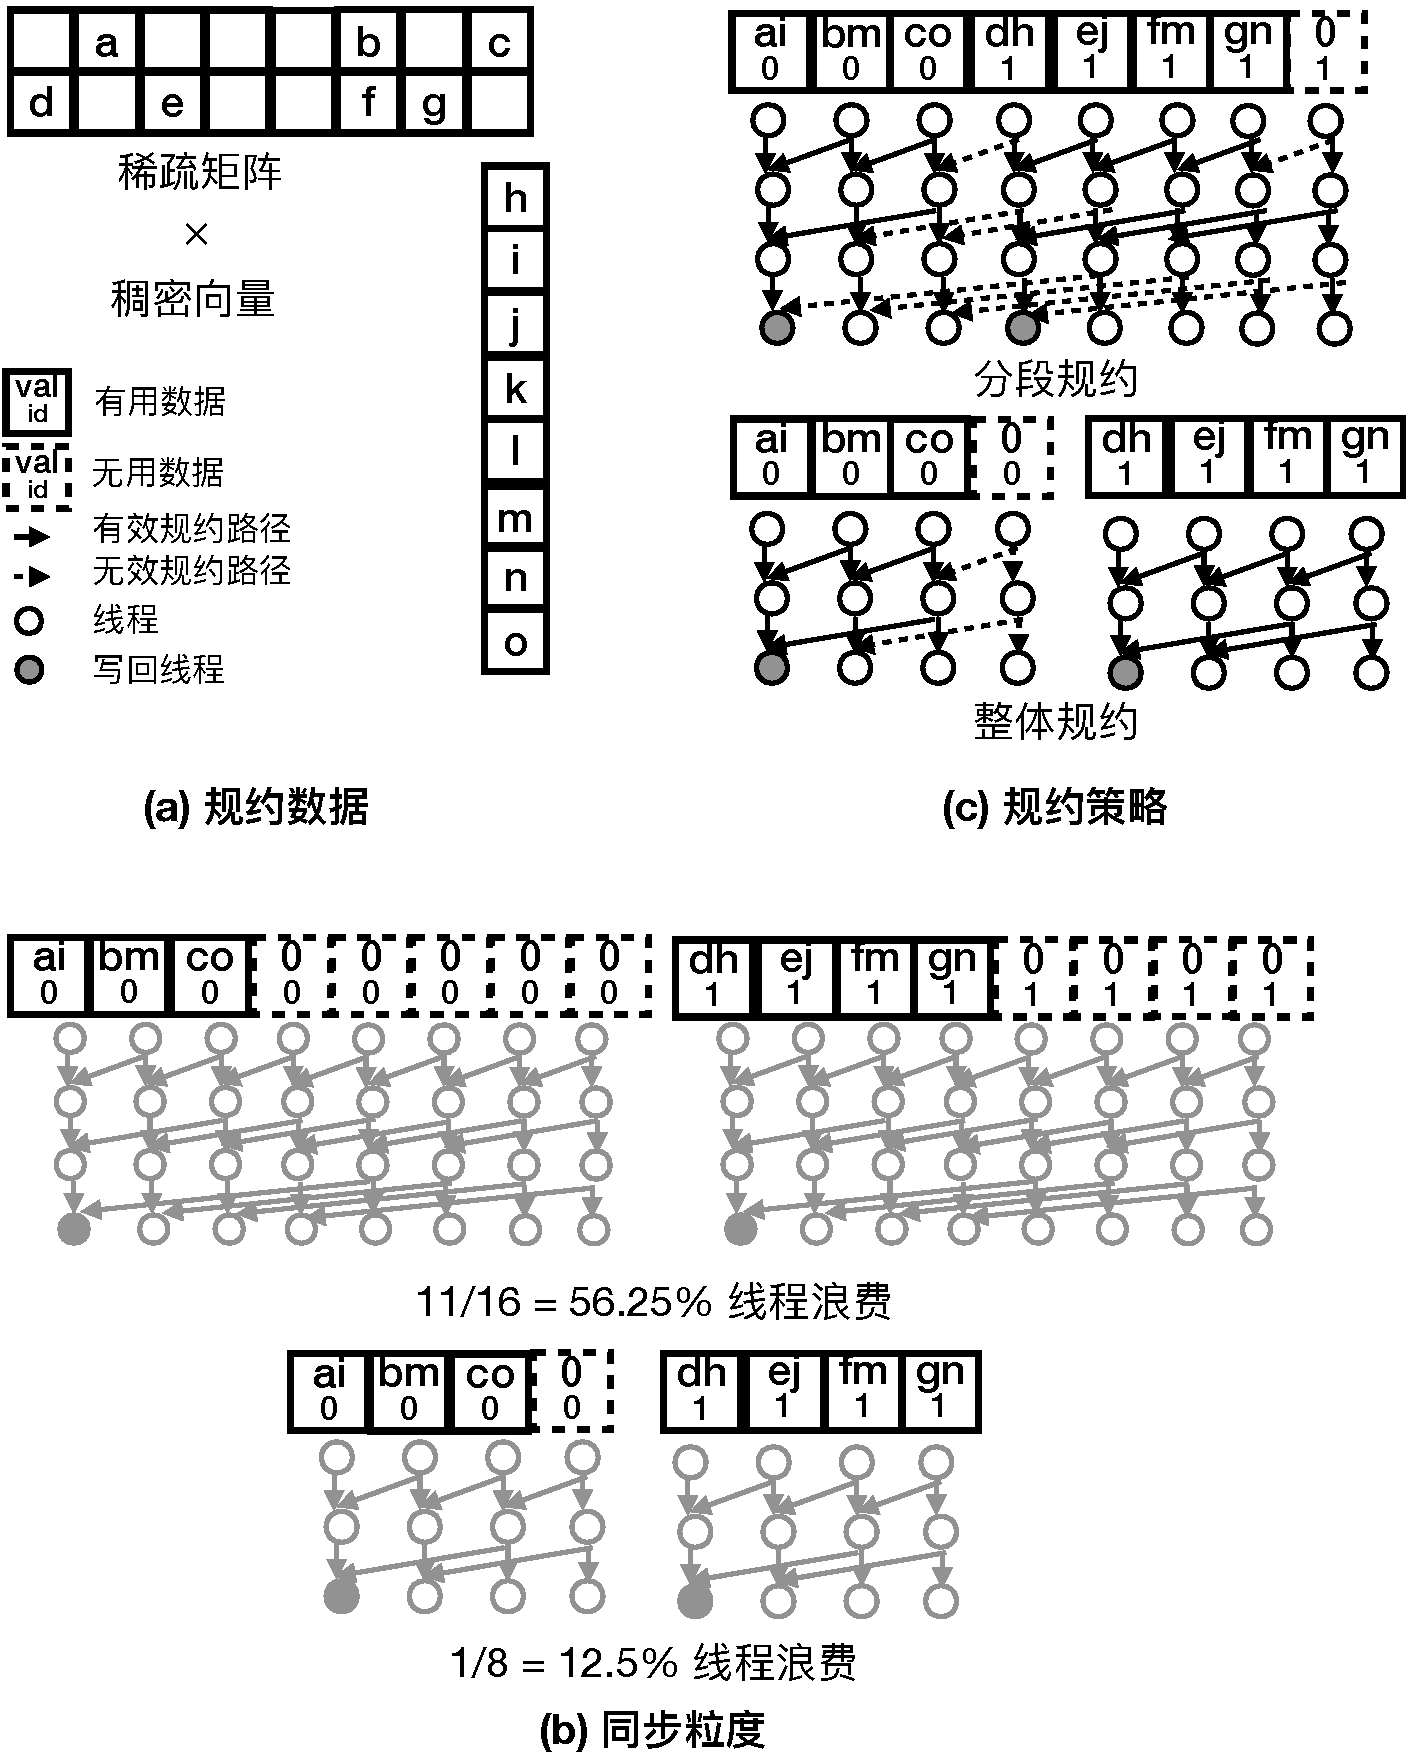
\includegraphics[width=0.5\textwidth]{reduction.pdf}
  \caption{不同规约粒度和规约方法示意图}
  \caption*{(a)被规约的数据。其中有一个行数为2列数为8的稀疏矩阵和一个长度为8的稠密向量做矩阵向量乘法。(b)不合适的规约粒度会导致线程浪费,该子图中未区分有效和无效规约路径。(c)分段规约和整体规约。在这个例子中分段规约有2个写回线程。整体规约始终只有1个写回线程。}
  \label{fig:reductions}
\end{figure}
同时,不同的规约粒度也可能影响线程利用率,进一步影响算子性能。PRedS\cite{yu2021exploiting}虽然研究了并行规约粒度对性能的影响,但是它只局限于$X$中所有元素的$id$相等的情况,即稠密规约。本文更进一步,研究稀疏规约,即$X$中元素的$id$不相等的情况。
因为$id$不相等,所以不是所有元素都要累加到同一个输出上。因此,本文引入了有用数据,无用数据,有效规约路径,无效规约路径,和写回线程等概念。
这些概念的产生与GPU的线程同步策略密切相关。GPU会同步一组线程,而这组线程的线程数是2的次方且不大于32。这组线程的线程数我们称之为同步粒度。线程可以向同一线程组的另一的线程种传递本线程持有的寄存器数据。有用数据的意思是对最后结果起作用的数据,即$X$中的元素。无用数据是规约粒度和待规约元素个数不匹配引入的数据。在图~\ref{fig:reductions}(b)的两个例子中,均采用整体规约。
因为整体规约要求所有被规约元素的$id$相同,所以当规约粒度超过$id$相同的元素数目时,就需要补充一些$val$是$\oplus$运算意义下的零元(在实数加法中就是0)的元素。这些元素只是起到占位作用,其$val$并没有加到输出结果中,因此被称为无用数据。
相应地,有效规约路径表示该路径连接的两种线程中,起始线程的值会最终叠加到写回线程的值中。无效规约路径则是为了避免GPU各线程执行路径不一致问题而引入的执行路径。
GPU提供了多种规约方式,写回线程表示该线程的寄存器中存放着最终写入$Out$的数据。分段规约表示一个线程组规约给定数目的$X$中的元素,整体规约表示一个线程组规约$X$中给定$id$的元素。分段规约根据该线程组处理的不同$id$数量可以有多个写回线程,整体规约因此$id$相同,所以只有1个写回线程。多个写回线程的线程号取决于$X$中的$id$分布,因此在运行时决定。两种规约的示意图如图~\ref{fig:reductions}(c)所示。
不同的输入数据适合不同的规约,比如在DA-SpMM\cite{dai2022heuristic}的对比实验中,分段规约和整体规约在不同数据集上的性能相比既可能好,也可能差2到4倍。

\section{灵活规约优化空间扩展}
\subsection{硬件模型}\label{sec:hwmodel}
因为规约是稀疏稠密混合张量代数的核心操作,所以优化空间扩展核心是多少数据需要被规约以及采用何种规约策略。本文将逻辑上原子的计算单元设置为线程。一个线程可以一个串行程序。所有线程独立执行相同的程序。每个线程有各自的输入数据,同时根据threadId区分。
线程可以成组做同步规约,规约并行度(粒度)可以是2,4,8,16或32.我们将GPU的计算建模为逻辑上无限多的平行线程,同时定义GPU可以提供的线程数为源并行度。在这个模型中我们没有考虑共享内存、线程块层级以及线程到流式处理器的映射策略等。本文把这些视作在基础并行模式确定后合理的部署细节。换句话说,在本文基于灵活规约扩展后的优化空间中,每一种优化策略对应许多不同的部署技术。这样扩展后的优化空间可以为GPU细节优化提供更简洁的视角。
\subsection{原子并行}\label{sec:atomicparallel}
为了具体定义并行模式,本文提出了原子并行概念。处于原子并行状态的一个程序不能继续被并行。换句话说,原子并行规定了一个线程执行的数据量。正式地,本文定义原子并行是最小数据的笛卡尔积。最小数据数据是一个线程所能处理的最小某类数据量。原子并行可以用来构建在GPU上执行的稀疏稠密混合代数的优化空间。
当然分块技术、精细管理共享内存、线程映射等优化技术对于GPU上的稀疏稠密混合代数也很重要\cite{hidayetouglu2020scale,mehrabi2021learning,xin2021fast,gale2020sparse}。这些技术对于稠密张量相对稀疏张量形状较大时更有利,比如在SpMM中稠密矩阵列数大于128时。因为计算的负载会很重,想稠密矩阵的向量化数据读取会成为瓶颈。
当稠密张量相对于稀疏张量形状较小,比如SpMM中稠密矩阵列数小于8时,每个线程的工作负载都较小,此时吞吐率被最长的线程组执行时钟数限制,因此需要更好的工作负载均衡。

下面以SpMM为例展示利用原子并行构建灵活规约优化空间扩展的步骤。SpMM有两种正交的原子并行:最小数据可以是$\{\frac{1}{g},1,g\}$个稀疏矩阵的非零元和$\{\frac{1}{c},1,c\}$个稠密矩阵列;也可以是$\{\frac{1}{g},1,g\}$个稀疏矩阵行和$\{\frac{1}{c},1,c\}$个稠密矩阵列。
其中$c\in \mathbb{Z^+}$和$g\in \mathbb{Z^+}$是可以调优的参数。尽管他们都可以是1但是他们和1的意义不同,因为他们是可以调优的。因此基于原子并行的SpMM灵活规约粒度优化空间扩展可以用$<x\,nnz , y\,col>$或者$<x\,row, y\,col>$描述。
源并行度只会向原子并行度中的一个元素做乘法。例如,给定源并行度$r$,针对第一种原子并行线程执行的数据量可以定义为$<r \times x\,nnz , y\,col>$或者$<x\,nnz, r \times y\,col>$;针对第二种原子并行线程执行的数据量可以定义为$<r \times x\,row , y\,col>$或者$<x\,row, r \times y\,col>$。
除此以外,分数类型的数据意味着不同线程会在同样的单个数据上执行。比如$<\frac{1}{g}\, row, 1\, col>$表示$g$个线程合作在同一行上执行。
\subsection{空间定义}\label{sec:spacedef}
依然使用SpMM的例子,我们用原子并行和规约并行 $\{<...>,r\}$ 来定义一个SpMM算子。$<...>\in \{\frac{1}{g},1,g\}\, nnz \times \{\frac{1}{c},1,c\}\, col $ or $\{\frac{1}{g},1,g\}\,row \times \{\frac{1}{c},1,c\}\,col$。他们描述了最小数据。同时规约并行度$r\in\{2,4,8,16,32\}$指定了每次有多少线程同步。 
图~\ref{fig:space3d}展示了SpMM的优化空间。但是,基于原子并行和规约并行构建的优化空间中不是所有点都合法。图~\ref{fig:space}中展示了空间剪枝的细节。优化空间中合法的点有3个条件:
\begin{enumerate}
  \item $\{<\frac{1}{g}\,nnz , x\,col>,r\}$, $\{<x\,nnz , \frac{1}{c}\,col>,r\}$ 
  是非法的,因为一个非零元一定与稠密矩阵中的一个点相乘。
  \item $\{<\frac{1}{g}\,row, x\,col>,r\}(\frac{r}{g}<1)$
  是非法的,因为整体规约只能有一个写回线程。
  \item $\{<\frac{1}{g}\,row , \frac{1}{c}\,col>,r\}$
  是非法的,因为它和源并行只能与原子并行中的一个元素相乘矛盾
\end{enumerate}
\begin{figure}[h]%
  \centering
  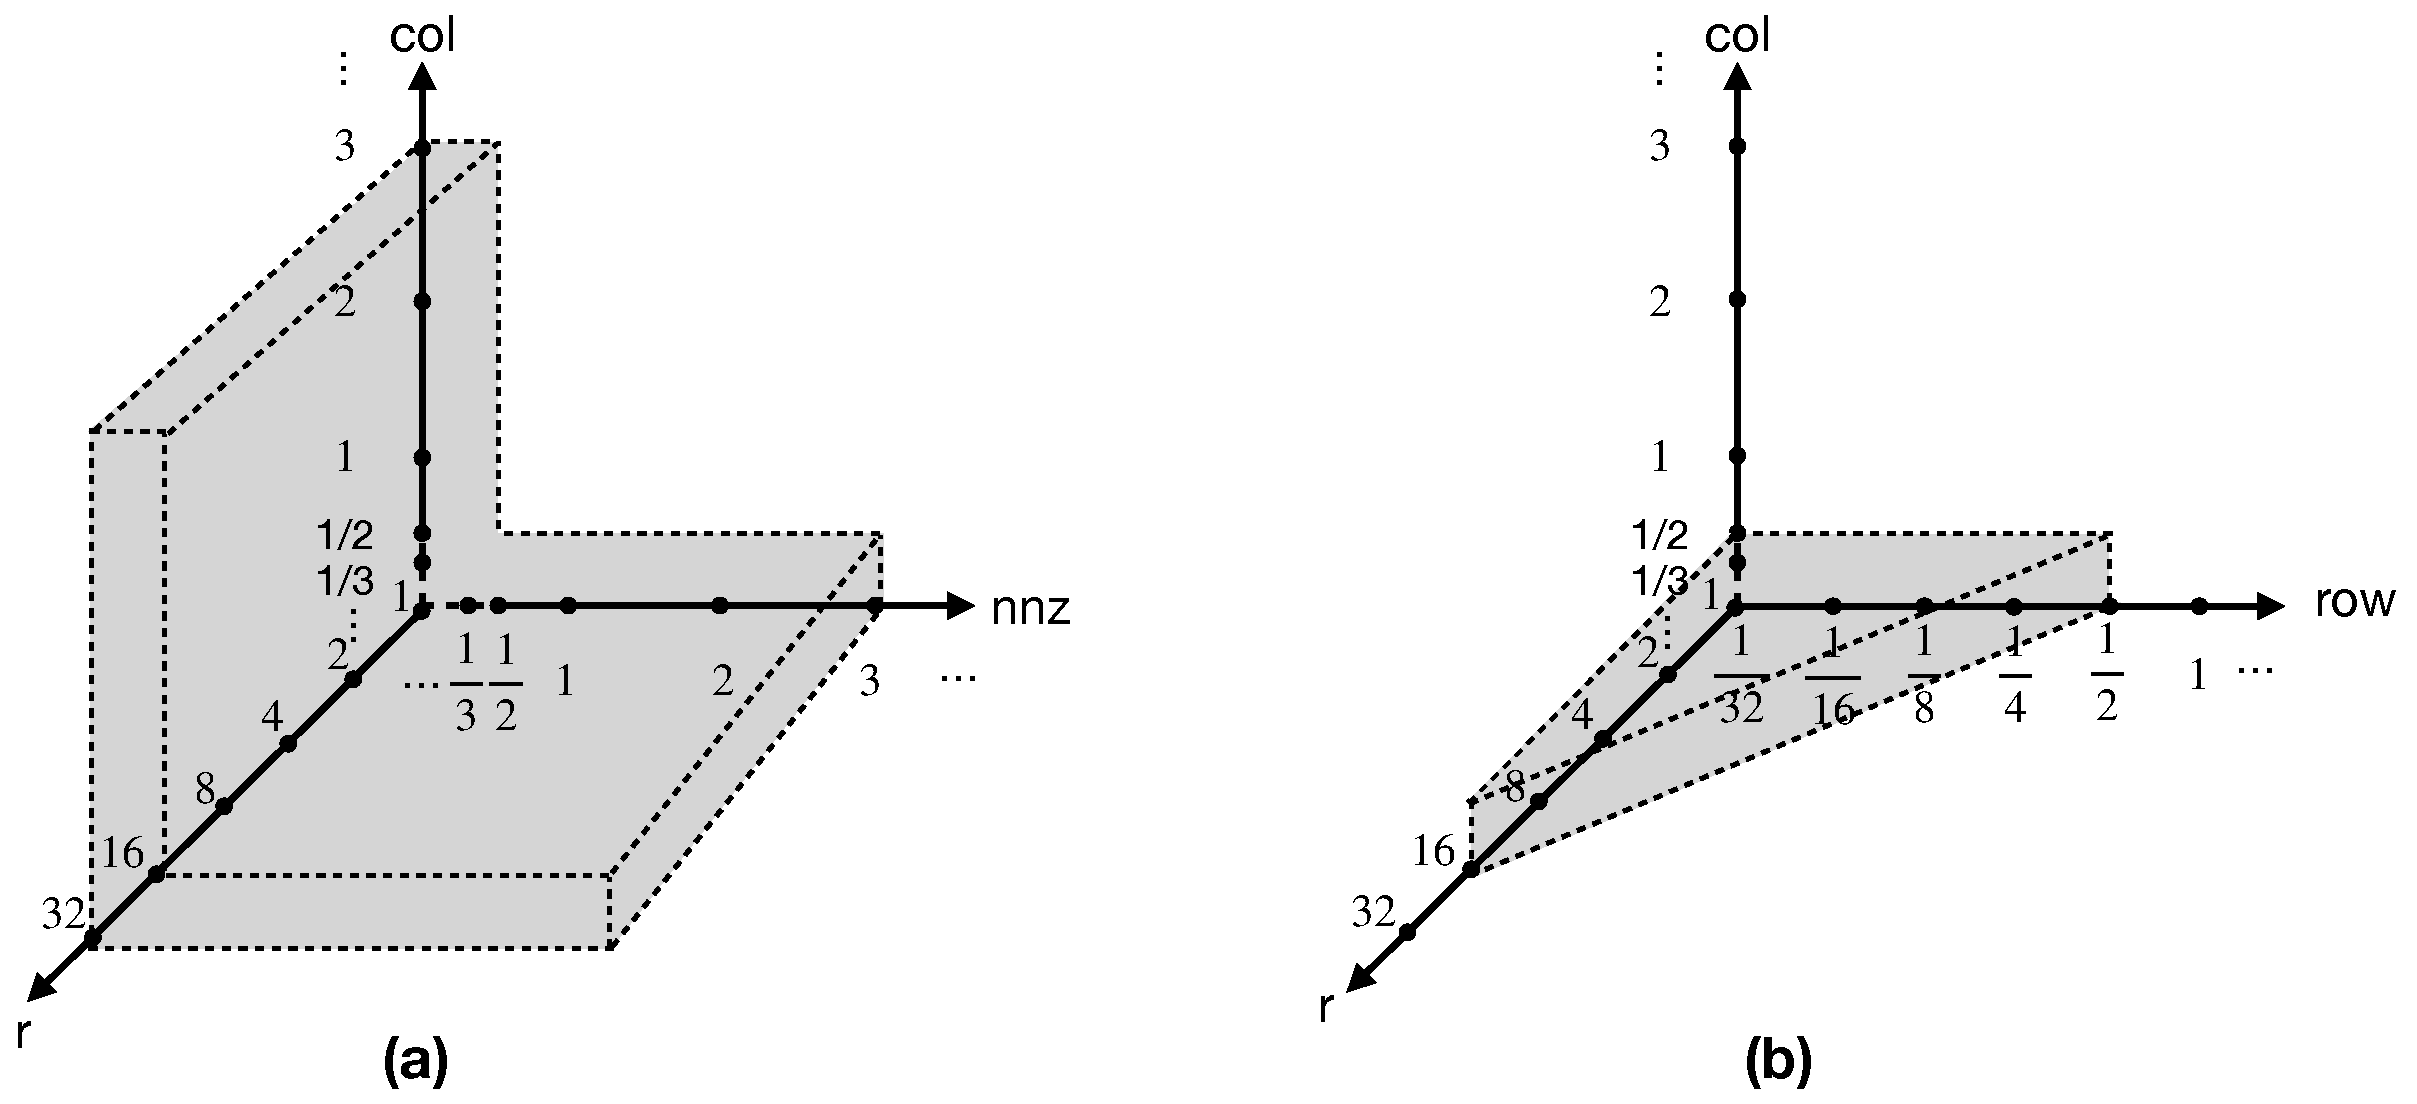
\includegraphics[width=0.9\textwidth]{space_3d.pdf}
  \caption{SpMM灵活规约优化空间扩展示意图}
  \caption*{灰色区域是非法区域,在每个坐标轴根部的虚线部分代表结束点和硬件相关。}
  \label{fig:space3d}
\end{figure}
\begin{figure}[h]%
  \centering
  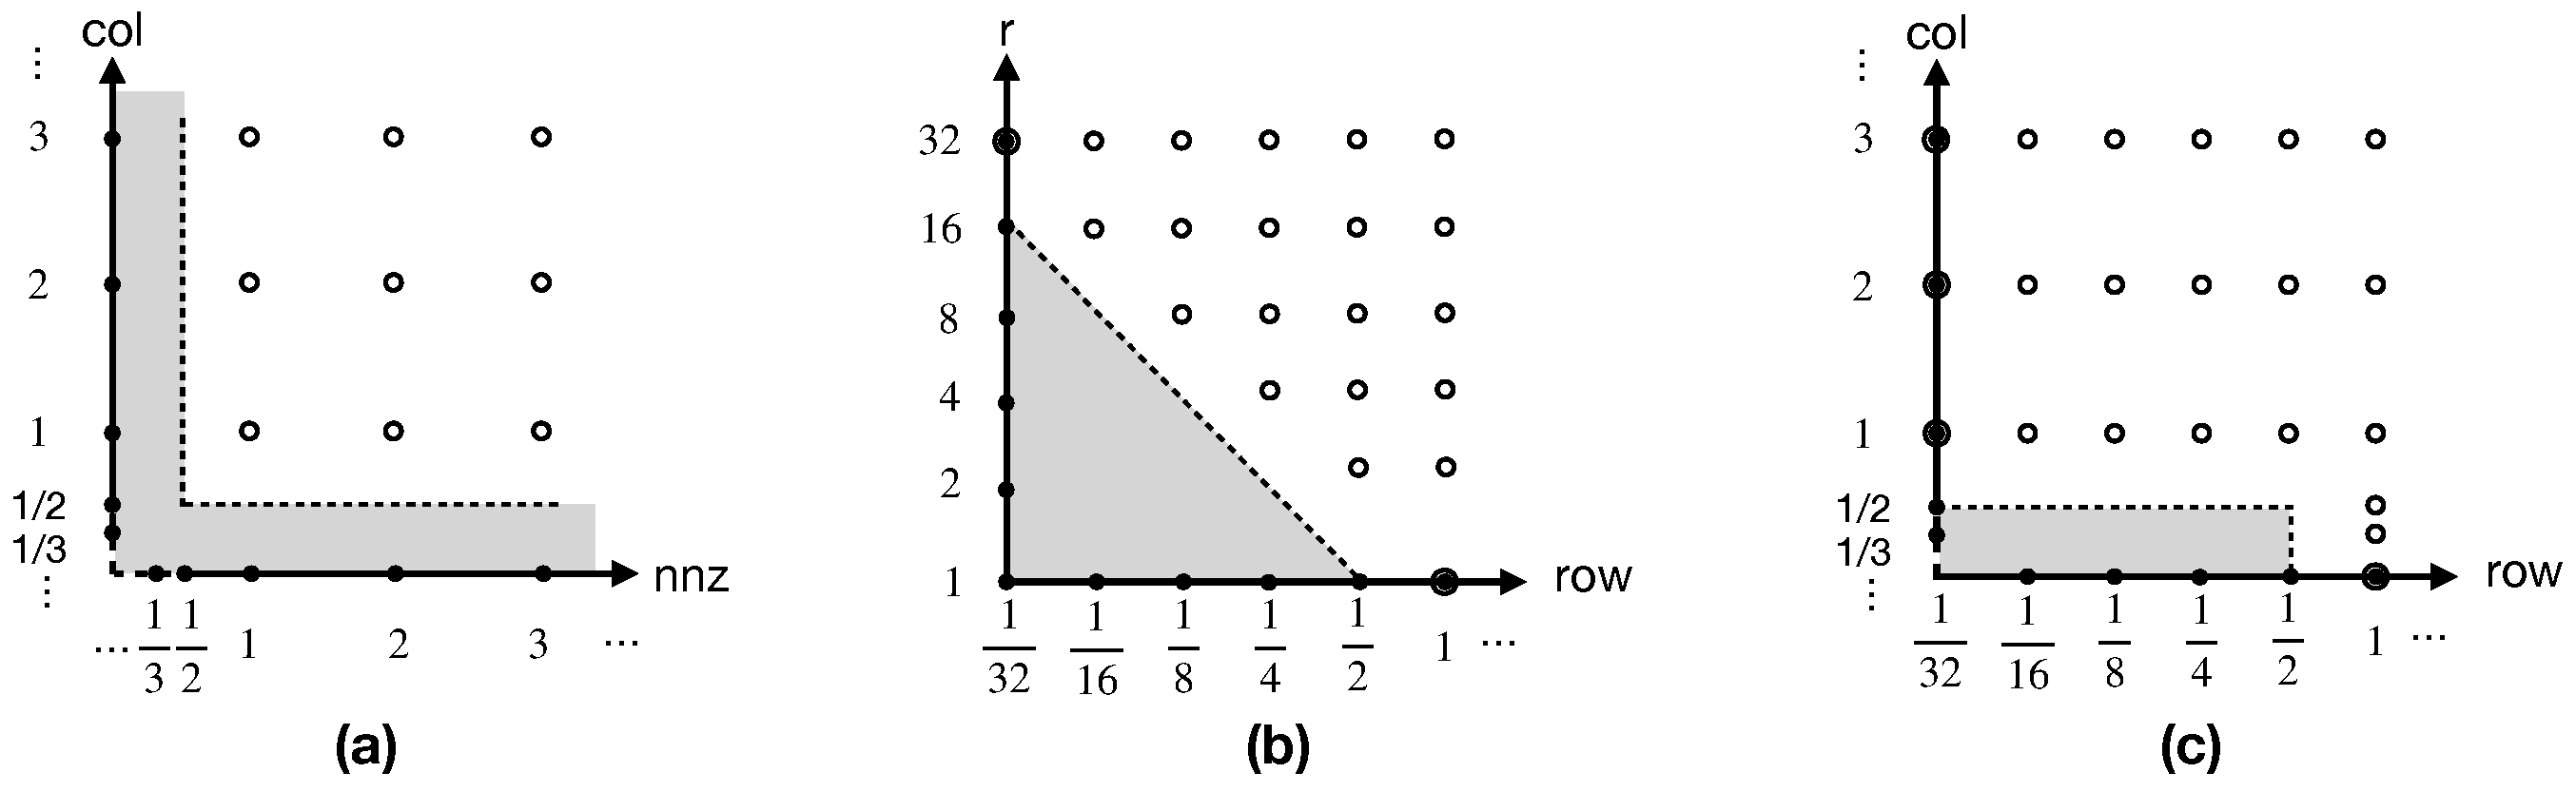
\includegraphics[width=0.9\textwidth]{space.pdf}
  \caption{SpMM灵活规约扩展优化空间的二维投影示意图}
  \caption*{灰色区域是非法的,空心圈是合法的点。子图(a),(b),(c)分别对应规则1,2,,3。}
  \label{fig:space}
\end{figure}
\begin{figure}[h]%
  \centering
  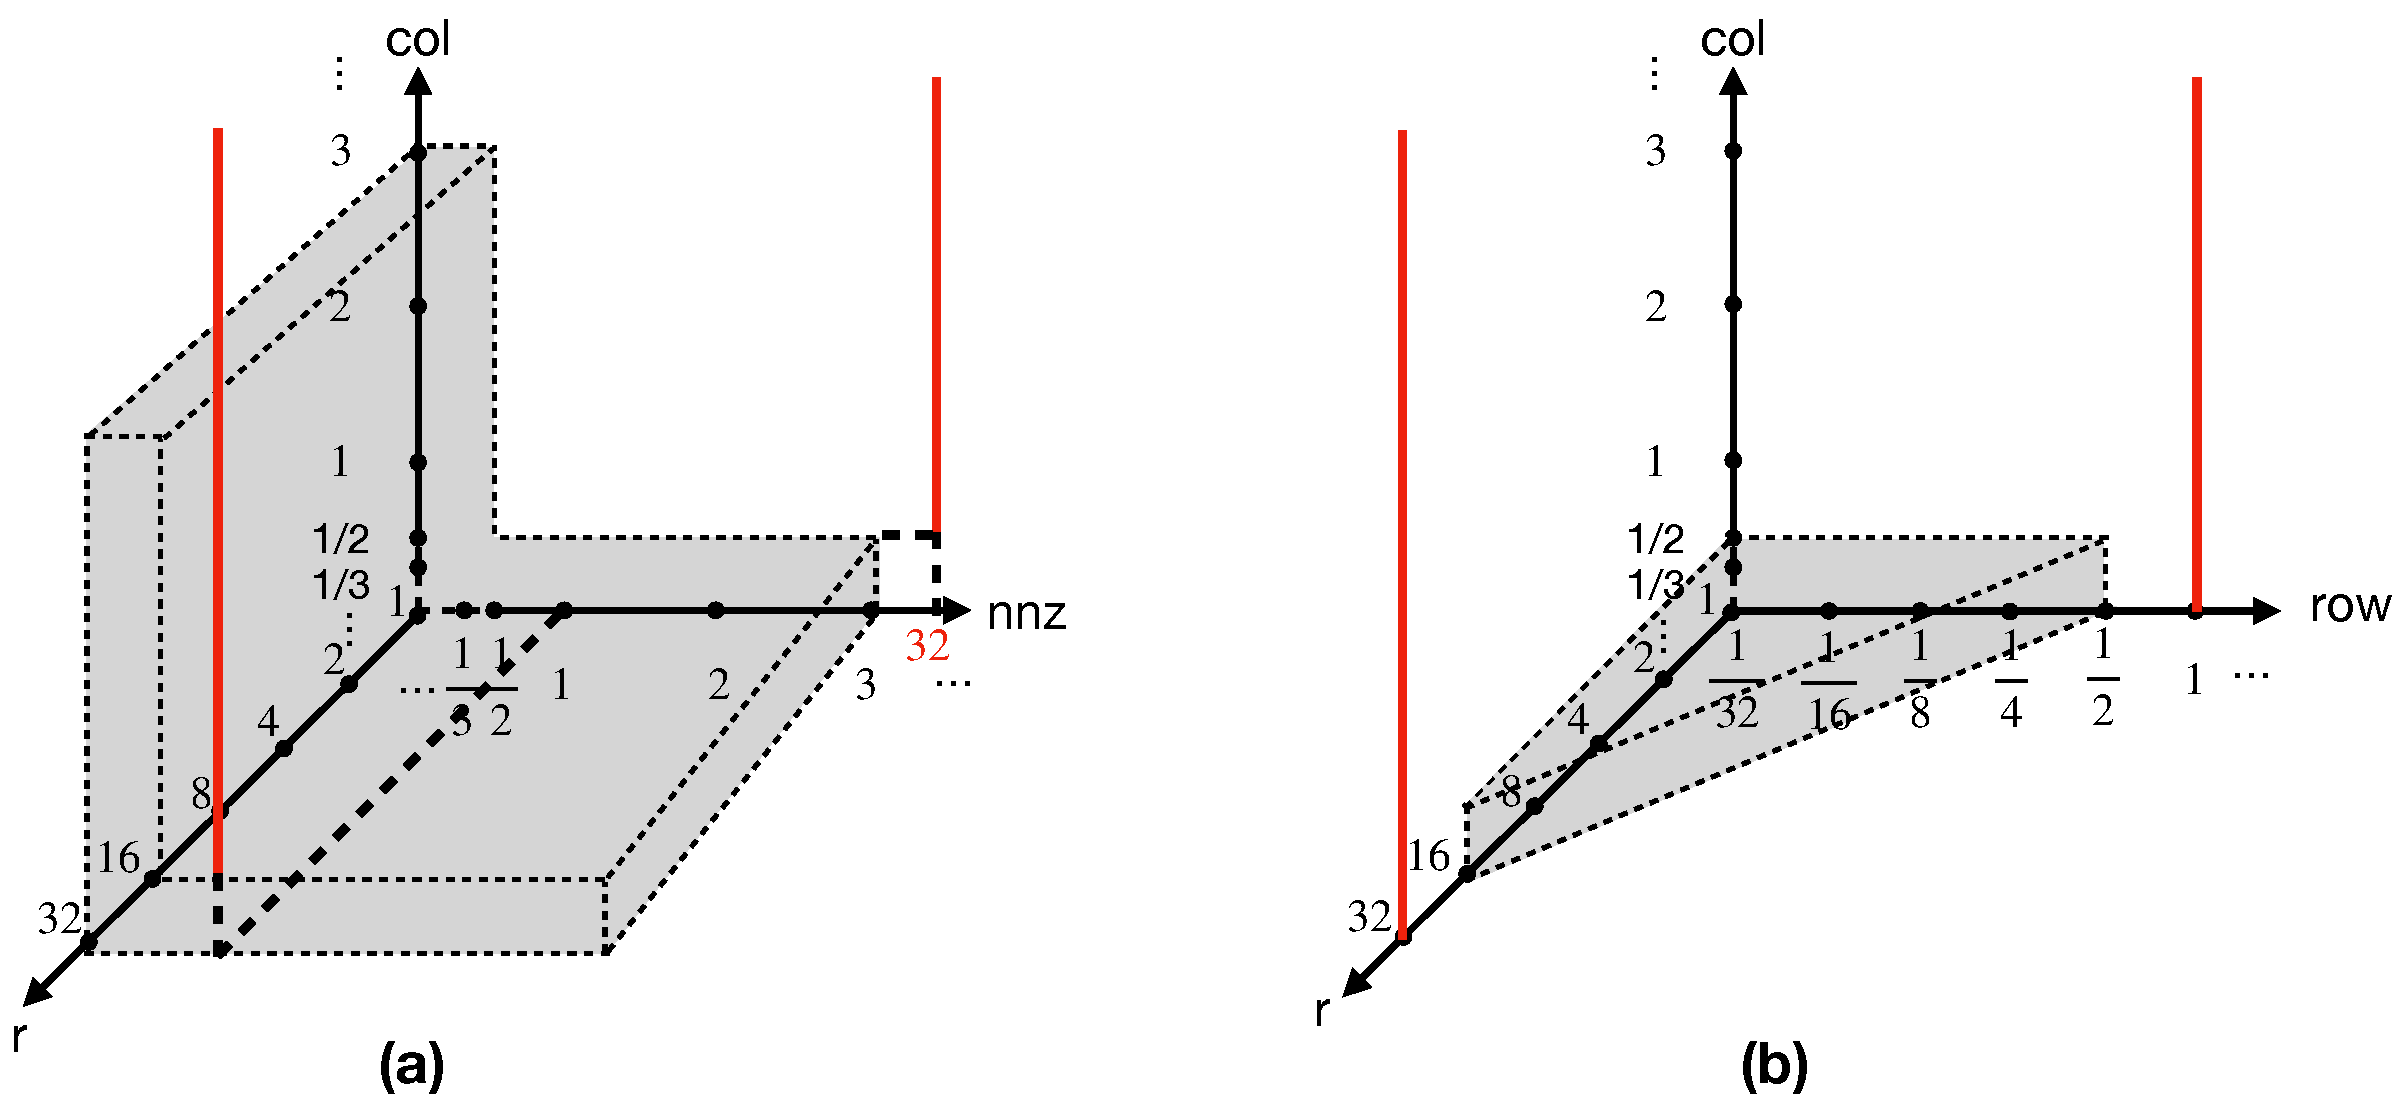
\includegraphics[width=0.9\textwidth]{daspmm.pdf}
  \caption{DA-SpMM的四种算法在灵活规约优化空间扩展中的位置}
  \caption*{红色代表DA-SpMM包含的优化空间,灰色区域是非法区域,在每个坐标轴根部的虚线部分代表结束点和硬件相关。}
  \label{fig:daspmm}
\end{figure}
最新的SpMM算子库设计空间DA-SpMM包含在上面基于原子并行构建的灵活规约优化空间扩展中。DA-SpMM提出了一个三维的SpMM算法设计空间,分别有三个维度:行/非零元均衡、行/列起始循环,并行/串行规约,论文中分别简称RB/EB、RM/CM、PR/SR。
因为行/列起始循环不影响并行策略,所以我们只考虑EB+PR,RB+PR,EB+SR,RB+SR四种算法。如图~\ref{fig:daspmm}所示,在灵活规约优化空间扩展中EB+PR是$\{<1\,nnz , c\,col>,32\}$,RB+PR是$\{<\frac{1}{32}\,row, c\,col>,32\}$,EB+SR是$\{<32\,nnz,c\,col >,1\}$,
RB+SR是$\{<1\,row,c\,col >,1\}$。其中$c$对应DA-SpMM中的向量化参数,$g$表示灵活规约中的线程组大小。尽管在真实GPU中由于源并行度有限,导致$1\,row$或$1\,nnz$可能会有超过1行或1个非零元的最小数据。但是我们仍然将这类算法归类为空间中的$1\,row$或$1\,nnz$点。


\section{实验结果}
\subsection{实验环境}\label{sec:exp-env}
本节在Turing(图灵),Volta(伏打)和Ampere(安培)三代GPU架构上进行算子性能测试,该三种架构分别对应RTX 2080,Tesla V100和RTX 3090:
\begin{itemize}
\item NVIDIA RTX 3090. Compute Capability 8.6 (68 Ampere SMs at 1.395 GHz, 24 GB GDDR6x, 936 GB/s bandwidth).
\item NVIDIA RTX 2080. Compute Capability 7.5 (46 Turing SMs at
1.515 GHz, 8 GB GDDR6, 448 GB/s bandwidth).
\item NVIDIA Tesla V100. Compute Capability 7.0 (80 Volta SMs at
1.370 GHz, 16 GB HBM2, 900 GB/s bandwidth). 
\end{itemize}
同时使用11.6版本的NVCC和11.6版本的CUDA,并采用和DA-SpMM相同的编译选项。我们用英伟达官方提供的nsight-compute\footnote{\url{https://docs.nvidia.com/nsight-compute/NsightCompute/index.html}}工具测试算子性能。数据集方面,和DA-SpMM选用相同数据集。
本文选择在三种架构上测试性能是为了展示灵活规约优化空间扩展可以不只局限于一种GPU架构,而是针对GPU所共有的SIMT架构都使用。
\subsection{实验部署}\label{sec:exp}
本文将灵活规约优化空间扩展部署到了dgSPARSE库。dgSPARSE库实现了DA-SpMM提出的8种SpMM算法,也实现了针对SDDMM的PRedS算法。这里采用和dgSPARSE一样的输入矩阵格式(CSR)。经过大量测量后本文发现RM算法始终比CM算法好。因此本节针对RM算法部署灵活规约扩展,也就是EB+SR+RM,EB+PR+RM,RB+SR+RM,RB+PR+RM。

如~\ref{sec:hwmodel}节所述,为了真实写出CUDA算子,我们需要比原子并行中规定的参数更细粒度的参数。在CUDA算子中,并行度被分为两层:线程块层次和线程层次,这一点和原子并行基于的同构线程模型是不一致的。
不仅如此,内存层级比如共享内存也需要考虑在内。同时,在真实GPU上并行度是首先的。比如,因为一个线程块最多包含1024个线程,所以最大的线程级别并行度就是1024.最大的线程块级别并行度也受限于流式处理器(SM)的数量。
当然,在编程时可以设置32位int数可以表示的任意大小的线程块并行度,但是实际执行时GPU的调度器会降超过SM数量的线程块之间串行处理。

上述问题是从原子并行模型中所有点到真实GPU可以执行的CUDA代码所共有的。下面以RB+PR+RM和EB+PR+RM为例介绍部署的细节。如~\ref{sec:spacedef}节中所述,RB+PR+RM在原子并行中表示为$\{<\frac{1}{g}\,row, c\,col>,r\}$,
EB+PR+RM在原子并行中表示为$\{<g\,nnz , c\,col>,r\}$。
首先介绍RB+PR+RM,该算子可调优的参数可以分为两类。一类是多少计算单元被分配给处理一段数据,包括\textit{blockSz},\textit{workerSz},\textit{workDimR}。第二类是多少块数据被分配给一个计算单元,包括\textit{tileSz},\textit{groupSz},\textit{threadRw},\textit{coarsenSz}。具体而言RB+PR+RM有7种可供调优的参数。
一个线程块处理\textit{tileSz}个稠密矩阵列。\textit{workerSz}个线程处理一个向量化的列和\textit{threadRw}个稀疏行。一个向量化的列包含\textit{coarsenSz}个连续的稠密列。
每次同步\textit{groupSz}个线程。每个线程块有\textit{blockSz}个线程。稀疏行的线程块并行度是\textit{workerDimR}。如果所有的稀疏行并行度小于稀疏矩阵中行的数目,那么一个线程可能会处理多行。在切分行的时候是行优先的,稠密列是全部并行的。
特别地,\textit{blockDim.x=min(N, tileSz) / coarsenSz * workerSz}。一个线程块的源并行度是\textit{max(blockSz, blockDim.x * 2)}。在dgSPARSE的部署中,\textit{tileSz = workerSz = groupSz = 32},\textit{workerDimR}等于稀疏矩阵行数,\textit{threadRw=1},
\textit{blockSz=256},同时\textit{coarsenSz=(N\%4==0)?4:(N\%2==0)?2:1}。

正如灵活规约扩展所指出的,我们应该将线程组的切分和同步语义分开讨论,添加细粒度并行度和每个线程灵活的工作负载。因此,我们需要调优4个参数:$<groupSz, blockSz, tileSz, workerDimR>$。
事实上\textit{workerDimR}可以被设置为任意正整数。但是我们把它设置为2的整数次幂或者2的负整数次幂乘之前的值来探索设计空间中一个较为局部的区域。正如我们在~\ref{sec:atomicparallel}节中
指出的那样,我们设置\textit{groupSz}为2,4,8,16,或32。\textit{tileSz}是2的次幂,同时比\textit{groupSz}大,并且和稠密矩阵列数$N$有关。\textit{blockSz}被设置为128,256,或512。
这些是每个线程块中常见的线程数。我们针对$N=4,16,64,128$对RB+PR+RM算子做性能调优。

现在介绍EB+PR+RM,类似在RB+PR+RM中,同样有7个两类参数。第一类参数,即多少计算单元被分配给处理一段数据,包括\textit{blockSz},\textit{workerSz},\textit{workDimNnz}。第二类参数,即多少块数据被分配给一个计算单元,包括\textit{tileSz},\textit{groupSz},\textit{threadNz},\textit{coarsenSz}。
与RB+PR+RM相同一个线程块处理\textit{tileSz}个稠密矩阵列。\textit{workerSz}个线程处理一个向量化的列,每次同步\textit{groupSz}个线程,每个线程块有\textit{blockSz}个线程。与前者不同的是,\textit{workerSz}个线程处理\textit{threadNz}个稀疏矩阵中非零元。
非零元的线程块并行度是\textit{workerDimNnz}。与前者类似,如果所有非零元的并行度小于稀疏矩阵中非零元数目,那么一个线程需要按照非零元并行度为步长循环非零元。在切分非零元时按照非零元的存储顺序切分,稠密列也是全部并行的。
因为$row$和$nnz$在原子并行中都是并行的一个维度,所以二者的调优参数有很多相似之处,不同点是$row$的并行数量可以是分数$\frac{1}{g}$,但是$nnz$的并行数量只能是整数。

\subsection{动态调优与开源算子库对比}\label{sec:overori}
因为DA-SpMM中介绍了一种决策树模型来针对一个给定的稀疏矩阵选择最好的参数配置,因此我们研究决策树的性能上限,即测试所有参数配置得到各个参数配置下的结果后,取最好的结果作为该算子的性能。这种测试方法称之为动态调优。比如,在$\{<g\,nnz , c\,col>,r\}$中,给定稠密矩阵列数和稀疏矩阵,测试了~\ref{sec:exp}节中提到的所有$g$,$c$,和$r$后,
选择最佳的性能,作为该稀疏算子在该稠密矩阵列数下的性能。这个实验目的是测试灵活规约优化空间扩展对算子库带来的性能提升,并研究设计一个动态模型在算子执行前自动选择最佳参数的必要性。
从表~\ref{tab:over-ori-eb}可以看出,针对$\{<g\,nnz , c\,col>,r\}$算法,随着稠密矩阵列数增大,平均计算速度提升比越大,说明性能调优的收益越大。
从表~\ref{tab:hw-eb}可以看出,在不同平台上的计算速度提升比相对差值在22\%以内,差别不大,说明灵活规约优化空间扩展在SIMT架构上具有适应性,而不局限在特定代的GPU架构。

\begin{table}
  \centering
  \caption{$\{<g\,nnz , c\,col>,r\}$算法相对于开源算子库的子集实现$\{<1\,nnz , c\,col>,32\}$的吞吐率提升比}
  \begin{tabular}{lllll}
  \toprule
  硬件平台 & 几何平均值  & 最大值 & 稠密矩阵列数 \\
  \midrule
  \multirow{4}{*}{RTX 3090}& 1.490  & 2.950  & 128\\
                          & 1.449   & 2.890  & 64\\
                          & 1.048   & 1.557  & 16\\
                          & 1.103   & 1.769 & 4\\
  \hline
  \multirow{4}{*}{RTX 2080}& 1.240   & 2.159  & 128\\
                          & 1.232   & 2.090  & 64\\
                          & 1.032   & 1.413  & 16\\
                          & 1.045   & 1.387  & 4\\
  \hline
  \multirow{4}{*}{Tesla V100}   & 1.505   & 3.519  & 128\\
                          & 1.469   & 3.398  & 64\\
                          & 1.040   & 1.511  & 16\\
                          & 1.084   & 1.732  & 4\\
  \bottomrule
  \end{tabular}
  \label{tab:over-ori-eb}%
\end{table}
\begin{table}
  \centering
  \caption{$\{<g\,nnz , c\,col>,r\}$算法动态调优与开源算子库吞吐率提升比针对不同代GPU的波动情况}
  \begin{tabular}{llllll}
  \toprule
  稠密矩阵列数 & $\frac{RTX\,3090}{RTX\,2080}$ & $\frac{RTX\,2080}{Tesla\,V100}$  & $\frac{Tesla\,V100}{RTX\,3090}$  & 最大波动比率 \\
  \midrule
  128 & 0.20 & 0.21 & 0.01 & 0.21 \\
  64  & 0.18 & 0.19 & 0.01 & 0.19 \\
  16  & 0.02 & 0.01 & 0.01 & 0.02 \\
  4   & 0.06 & 0.04 & 0.02 & 0.06 \\
  \bottomrule
  \end{tabular}
  \label{tab:hw-eb}
\end{table}
从表~\ref{tab:over-ori-rb}可以看出,针对$\{<\frac{1}{g}\,row , c\,col>,r\}$算法,随着稠密矩阵列数增大,平均计算速度提升比不一定越大。
从表~\ref{tab:hw-rb}可以看出,在不同平台上的计算速度提升比相对差值在26\%以内,较$\{<g\,nnz , c\,col>,r\}$算法相对波动大。
\begin{table}
  \centering
  \caption{$\{<\frac{1}{g}\,row , c\,col>,r\}$算法相对于开源算子库的子集实现$\{<\frac{1}{32}\,row , c\,col>,32\}$的吞吐率提升比}
  \begin{tabular}{lllll}
  \toprule
  硬件平台 & 几何平均值  & 最大值 & 稠密矩阵列数 \\
  \midrule
  \multirow{4}{*}{RTX 3090}& 2.295   & 4.316  & 128\\
                          & 2.181   & 4.432  & 64\\
                          & 1.997   & 4.271  & 16\\
                          & 2.046   & 7.819  & 4\\
  \hline
  \multirow{4}{*}{RTX 2080}& 1.938   & 4.379  & 128\\
                          & 1.927   & 4.430  & 64\\
                          & 1.995   & 5.019  & 16\\
                          & 2.307   & 8.582  & 4\\
  \hline
  \multirow{4}{*}{Tesla V100}   & 1.874   & 3.724  & 128\\
                          & 1.824   & 3.846  & 64\\
                          & 1.693   & 3.388  & 16\\
                          & 1.852   & 6.114  & 4\\
  \bottomrule
  \end{tabular}
  \label{tab:over-ori-rb}%
\end{table}
\begin{table}
  \centering
  \caption{$\{<\frac{1}{g}\,row , c\,col>,r\}$算法动态调优与开源算子库吞吐率提升比针对不同代GPU的波动情况}
  \begin{tabular}{llllll}
  \toprule
  稠密矩阵列数 & $\frac{RTX\,3090}{RTX\,2080}$ & $\frac{RTX\,2080}{Tesla\,V100}$  & $\frac{Tesla\,V100}{RTX\,3090}$  & 最大波动比率 \\
  \midrule
  128 & 0.18 & 0.03 & 0.22 & 0.22 \\
  64  & 0.13 & 0.06 & 0.20 & 0.20 \\
  16  & 0.001 & 0.18 & 0.18 & 0.18 \\
  4   & 0.13 & 0.25 & 0.11 & 0.25 \\
  \bottomrule
  \end{tabular}
  \label{tab:hw-rb}
\end{table}


\subsection{动态调优和静态选择对比}\label{sec:dystd}
~\ref{sec:overori}节说明了动态调优可以带来性能提升,在$\{<g\,nnz , c\,col>,r\}$上可以提升1.04到1.49倍,在$\{<\frac{1}{g}\,row , c\,col>,r\}$上可以提升
1.693到2.295倍。但是,这些证据还不足以支持使用动态调优。因为可能存在一个或几个参数配置始终性能很好。因此本节测试静态选择和动态调优的性能对比。静态选择指采用一种参数配置。
最佳静态配置指,采用该种配置后,与其他配置相比,在所有测试稀疏矩阵上,动态调优与之相比性能提升最小。
\begin{table}
  \centering
  \caption{$\{<g\,nnz , c\,col>,r\}$算法动态调优和静态选择吞吐率对比}
  \begin{tabular}{lllll}
  \toprule
  硬件平台 & 几何平均值  & 稠密矩阵列数 & 最佳静态配置 \\
  \midrule
  \multirow{5}{*}{RTX 3090}& 1.041  & 128 & (32, 256, 32, 1/32)\\
                          & 1.044   & 128 & (32, 256, 32, 1/16)\\
                          & 1.048   & 64 & (32, 256, 32, 1/8)\\
                          & 1.048   & 16 & (32, 256, 32, 1/8)\\
                          & 1.059   & 4 & (32, 256, 32, 1/4)\\
  \hline
  \multirow{6}{*}{RTX 2080}& 1.026  & 128 & (32, 256, 32, 1/32)\\
                          & 1.024   & 128 & (32, 256, 32, 1/16)\\
                          & 1.033   & 64 & (32, 256, 32, 1/16)\\
                          & 1.033   & 16 & (32, 256, 32, 1/16)\\
                          & 1.032   & 16& (32, 256, 32, 1/8)\\
                          & 1.050   & 4 & (32, 256, 32, 1/8)\\
  \hline
  \multirow{5}{*}{Tesla V100}& 1.028  & 128 & (32, 256, 32, 1/32)\\
                          & 1.029   & 128 & (32, 256, 32, 1/16)\\
                          & 1.029   & 64 & (32, 256, 32, 1/16)\\
                          & 1.040   & 16 & (32, 256, 32, 1/8)\\
                          & 1.053   & 4 & (32, 256, 32, 1/4)\\
  \bottomrule
  \end{tabular}
  \label{tab:over-sta-eb}
\end{table}
表~\ref{tab:over-sta-eb}中最佳静态配置的括号中4个参数分别指\textit{groupSz},\textit{blockSz},\textit{tileSz},$\frac{workerDimNnz}{rows}$其中\textit{rows}是稀疏矩阵行数。
从中可以看到,$\{<g\,nnz , c\,col>,r\}$的优化空间中性能较高的点几乎集中在(32, 256, 32, 1/32),这与DA-SpMM的(32, 256, 32, 1)只在总并行度有区别。因此针对这种工作负载,DA-SpMM的配置距离
经过灵活规约扩展后的空间中最优点很近。这说明非零元均衡可以较好平衡负载,因此最小数据和规约并行度一致时性能较好,且规约并行度越大性能越好。32是GPU提供的最大线程组规约并行度。
\begin{table}
  \centering
  \caption{$\{<\frac{1}{g}\,row , c\,col>,r\}$算法动态调优和静态选择吞吐率对比}
  \begin{tabular}{lllll}
  \toprule
  硬件平台 & 几何平均值  & 稠密矩阵列数 & 最佳静态配置 \\
  \midrule
  \multirow{4}{*}{RTX 3090}& 1.124  & 128 & (8, 256, 8, 1/2)\\
                          & 1.152   & 64 & (8, 256, 8, 1/2)\\
                          & 1.310   & 16 & (8, 256, 8, 1/2)\\
                          & 1.406   & 4 & (8, 256, 8, 1)\\
  \hline
  \multirow{4}{*}{RTX 2080}& 1.095  & 128 & (4, 256, 8, 1/2)\\
                          & 1.114   & 64 & (4, 256, 8, 1/2)\\
                          & 1.276   & 16& (4, 256, 8, 1/2)\\
                          & 1.310   & 4 & (4, 256, 8, 1/2)\\
  \hline
  \multirow{4}{*}{Tesla V100}& 1.137  & 128 & (8, 256, 8, 1/2)\\
                          & 1.177   & 64 & (4, 256, 8, 1/2)\\
                          & 1.367   & 16 & (8, 256, 8, 1)\\
                          & 1.326   & 4 & (8, 256, 8, 1)\\
  \bottomrule
  \end{tabular}
  \label{tab:over-sta-rb}
\end{table}
表~\ref{tab:over-sta-rb}中最佳静态配置的括号中4个参数分别指\textit{groupSz},\textit{blockSz},\textit{tileSz},$\frac{workerDimR}{rows}$。
从中可以看到,$\{<\frac{1}{g}\,row , c\,col>,r\}$的优化空间性质和$\{<g\,nnz , c\,col>,r\}$不同,规约并行度为8更适合这种算法。因为每行非零元分布不一致,所以行均衡不易做到每个并行单元负载均衡,
因此不能保证规约并行度越大性能越好。规约并行度过大会造成过多无效规约路径,降低线程利用率。规约并行度过小会造成程序并行度低,并导致对GPU并行度利用率不足,也会损害算子性能。


\subsection{静态选择与开源算子库对比}
本节探究静态选择与开源算子库的性能比较。~\ref{sec:overori}节探究了动态调优对开源算子库的性能提升,说明了灵活规约优化空间扩展的有效性;~\ref{sec:dystd}节探究了动态调优对静态选择的性能提升,衡量了添加动态选择模型的必要性,但是二者的结果还不足以衡量实际应用时灵活规约带来的性能收益。
因为在DA-SpMM的开源库中没有动态选择模型,所以本节希望测试用静态选择的最佳参数配置直接替换开源算子库中对应算子,观测性能提升。
从表~\ref{tab:sta-ori-eb}中可以看出$\{<g\,nnz , c\,col>,r\}$直接用静态选择替换EB+PR+RM算子,可以给算子库平均带来1.090到1.463倍的性能提升。
\begin{table}
  \centering
  \caption{$\{<g\,nnz , c\,col>,r\}$算法静态选择和开源算子库吞吐率对比}
  \begin{tabular}{llllll}
  \toprule
  硬件平台 & 平均值 & 几何平均值  & 稠密矩阵列数 & 最佳静态配置 \\
  \midrule
  \multirow{5}{*}{RTX 3090}& 1.465 & 1.431  & 128 & (32, 256, 32, 1/32)\\
                           & 1.455 & 1.426  & 128 & (32, 256, 32, 1/16)\\
                           & 1.401 & 1.383  & 64 & (32, 256, 32, 1/8)\\
                           & 1.327 & 1.310  & 16 & (32, 256, 32, 1/8)\\
                           & 1.200 & 1.185  & 4 & (32, 256, 32, 1/4)\\
  \hline
  \multirow{6}{*}{RTX 2080}& 1.226 & 1.209 & 128 & (32, 256, 32, 1/32)\\
                           & 1.226 & 1.211 & 128 & (32, 256, 32, 1/16)\\
                           & 1.217 & 1.202 & 64 & (32, 256, 32, 1/16)\\
                           & 1.184 & 1.169 & 16 & (32, 256, 32, 1/16)\\
                           & 1.180 & 1.170  & 16& (32, 256, 32, 1/8)\\
                           & 1.100 & 1.090  & 4 & (32, 256, 32, 1/8)\\
  \hline
  \multirow{5}{*}{Tesla V100}& 1.528 & 1.463 & 128 & (32, 256, 32, 1/32)\\
                             & 1.517 & 1.462 & 128 & (32, 256, 32, 1/16)\\
                             & 1.482 & 1.427  & 64 & (32, 256, 32, 1/16)\\
                             & 1.353 & 1.316  & 16 & (32, 256, 32, 1/8)\\
                             & 1.166 & 1.144  & 4 & (32, 256, 32, 1/4)\\
  \bottomrule
  \end{tabular}
  \label{tab:sta-ori-eb}
\end{table}
从表~\ref{tab:sta-ori-rb}中可以看出$\{<\frac{1}{g}\,row , c\,col>,r\}$直接用静态选择替换RB+PR+RM算子,可以给算子库带来平均1.238到2.042倍的性能提升。
\begin{table}
  \centering
  \caption{$\{<\frac{1}{g}\,row , c\,col>,r\}$算法静态选择和和开源算子库吞吐率对比}
  \begin{tabular}{llllll}
  \toprule
  硬件平台 & 几何平均值  & 稠密矩阵列数 & 最佳静态配置 \\
  \midrule
  \multirow{4}{*}{RTX 3090}& 2.279 & 2.042  & 128 & (8, 256, 8, 1/2)\\
                           & 2.163 & 1.892  & 64 & (8, 256, 8, 1/2)\\
                           & 1.868 & 1.524  & 16 & (8, 256, 8, 1/2)\\
                           & 1.854 & 1.456  & 4 & (8, 256, 8, 1)\\
  \hline
  \multirow{4}{*}{RTX 2080}& 1.915 & 1.770  & 128 & (4, 256, 8, 1/2)\\
                          & 1.887 & 1.729   & 64 & (4, 256, 8, 1/2)\\
                          & 1.759 & 1.563  & 16& (4, 256, 8, 1/2)\\
                          & 2.178 & 1.762   & 4 & (4, 256, 8, 1/2)\\
  \hline
  \multirow{4}{*}{Tesla V100}& 1.826 & 1.647  & 128 & (8, 256, 8, 1/2)\\
                          & 1.746 & 1.550   & 64 & (4, 256, 8, 1/2)\\
                          & 1.431 & 1.238  & 16 & (8, 256, 8, 1)\\
                          & 1.731 & 1.397  & 4 & (8, 256, 8, 1)\\
  \bottomrule
  \end{tabular}
  \label{tab:sta-ori-rb}
\end{table}

\subsection{动态调优与官方算子库对比}\label{sec:overcu}
本节对比灵活规约扩展后的优化空间和官方闭源算子库的性能。优势矩阵表示灵活规约扩展比官方算子库吞吐率低的算子的稀疏矩阵。从表~\ref{tab:dy-cusp-eb}中可以看到当稠密矩阵列数增大时,优势矩阵个数减少,平均相对性能也更低,这说明$\{<g\,nnz , c\,col>,r\}$数据流更适用于稠密矩阵列数小于64的情况。
从表~\ref{tab:dy-cusp-rb}中可以发现,同样地当稠密矩阵列数增大时,优势矩阵个数减少,平均相对性能也更低。
\begin{table}
  \centering
  \caption{$\{<g\,nnz , c\,col>,r\}$算法动态调优和和官方算子库吞吐率对比}
  \begin{tabular}{llllll}
  \toprule
  硬件平台 & 几何平均值 & 最大值  & 稠密矩阵列数 & 优势矩阵个数 \\
  \midrule
  \multirow{4}{*}{RTX 3090}& 0.342 & 1.394  & 128 & 1\\
                           & 0.371 & 2.451  & 64 & 1\\
                           & 1.068 & 9.474  & 16 & 401\\
                           & 3.123 & 31.75  & 4 & 740\\
  \hline
  \multirow{4}{*}{RTX 2080}& 0.263 & 0.881  & 128 & 0\\
                          & 0.303 & 1.473   & 64 & 1\\
                          & 0.922 & 5.884  & 16 & 278\\
                          & 2.643 & 19.37  & 4 & 740\\
  \hline
  \multirow{4}{*}{Tesla V100}& 0.295 & 2.022  & 128 & 1\\
                          & 0.303 & 3.758  & 64 & 2\\
                          & 1.165 & 14.46  & 16 & 518\\
                          & 3.016 & 45.23  & 4 & 740\\
  \bottomrule
  \end{tabular}
  \label{tab:dy-cusp-eb}
\end{table}
从表~\ref{tab:dy-cusp-eb-sr}可以发现,规约并行度是1时,灵活规约扩展优化空间也可相比算子库取得1.343到3.341倍的加速。
\begin{table}
  \centering
  \caption{$\{<\frac{1}{g}\,row , c\,col>,r\}$算法静态选择和和官方算子库对比}
  \begin{tabular}{llllll}
  \toprule
  硬件平台 & 几何平均值 & 最大值 & 稠密矩阵列数 & 优势矩阵个数 \\
  \midrule
  \multirow{4}{*}{RTX 3090}& 0.499 & 2.256 & 128 & 1\\
                           & 0.520 & 3.633 & 64 & 5\\
                           & 1.470 & 17.02 & 16 & 602\\
                           & 4.150 & 61.80 & 4 & 685\\
  \hline
  \multirow{4}{*}{RTX 2080}& 0.327 & 1.130 & 128 & 1\\
                          & 0.371 & 1.969  & 64 & 1\\
                          & 1.162 & 8.206  & 16 & 525\\
                          & 3.861 & 38.039 & 4 & 694\\
  \hline
  \multirow{4}{*}{Tesla V100}& 0.374 & 2.682 & 128 & 1\\
                          & 0.494 & 4.981  & 64 & 4\\
                          & 1.406 & 18.73  & 16 & 607\\
                          & 3.922 & 86.353  & 4 & 688\\
  \bottomrule
  \end{tabular}
  \label{tab:dy-cusp-rb}
\end{table}
\begin{table}
  \centering
  \caption{$\{<g\,nnz , c\,col>,1\}$算法动态调优和和官方算子库吞吐率对比}
  \begin{tabular}{llllll}
  \toprule
  硬件平台 & 几何平均值 & 最大值  & 稠密矩阵列数 & 优势矩阵个数 \\
  \midrule
  \multirow{3}{*}{RTX 3090}& 1.343 & 11.157 & 64 & 737\\
                           & 2.181 & 23.147  & 16 & 740\\
                           & 3.188 & 32.356  & 4 & 738\\
  \hline
  \multirow{3}{*}{RTX 2080}& 1.212 & 6.804  & 64 & 696\\
                          & 1.871 & 12.375  & 16 & 740\\
                          & 2.851 & 22.108  & 4 & 738\\
  \hline
  \multirow{3}{*}{Tesla V100}& 1.400 & 14.384  & 64 & 730\\
                          & 2.218 & 29.566 & 16 & 740\\
                          & 3.341 & 50.998  & 4 & 738\\
  \bottomrule
  \end{tabular}
  \label{tab:dy-cusp-eb-sr}
\end{table}
% !TeX root = ../thuthesis-example.tex

\chapter{编译算法优化}
\thusetup{
  cite-style = super,
}

\section{灵活规约语义提升}\label{sec:compiler-alg-intro}
首先,~\ref{sec:reduction-core}节证明了规约是稀疏稠密混合代数的核心操作。稀疏稠密混合代数包括诸如SpMM,SDDMM,MTTKRP,TTM等多种算子。从这一核心观察出发,基于~\ref{sec:hwmodel}节描述的硬件模型,和~\ref{sec:atomicparallel}节提出的原子并行来定义并行模式。
之后基于硬件模型和原子并行提出了灵活规约优化空间扩展,并以SpMM为例展示了空间扩展的构建方式。之后对灵活规约的实际性能提升做了详细的实验验证。~\ref{sec:overori}节证明了优化空间中的$\{<\frac{1}{g}\,row , c\,col>,r\}$区域和$\{<g\,nnz , c\,col>,r\}$区域经过灵活
规约扩展后可以提升原有算子的性能,~\ref{sec:overcu}节证明了灵活规约扩展后的优化空间包含性能超过官方算子库的算子。但是,~\ref{sec:exp}节的算子是人工手写的,如果向不同稀疏稠密混合代数应用灵活规约技术,需要大量工程成本,但是之前又已经通过分析
论证了灵活规约可以加速这些稀疏稠密混合代数算子。为了能以较低的成本获得灵活规约带来的性能收益,本文提出了基于灵活规约语义提升技术。这是一种基于灵活规约的编译算法,可以对任何稀疏稠密混合代数快速构建优化空间,并提供方便的性能调优接口。

当前有CUDA后端代码生成的稀疏张量编译器将线程组的语义规定为:在分块中线程的一个层级即分块语义,一个特定的并行计算单元即同步语义,或者只是一个硬件指令即硬件性质语义。例如,TACO假设将一个循环变量拆分后得到的外循环变量
设置为线程组,内循环变量设置为线程,此时线程组的大小就是分块的参数。在这里,线程组被规定为分快中线程的一个层级,没有同步语义。同时,TACO将32线程大小的线程组作为一个执行原子加法的
并行计算单元,同时假设用户在使用这一原子加法并行单元时会将最后一层循环以32为粒度拆分。在这里,线程组的执行行为是以1为步长,循环次数为32次的for循环规约。在TACO后端,一段CUDA的线程组元语比如
\textit{\_\_shfl\_down\_sync}会被发射作为上层线程组规约语义的底层实现。图~\ref{fig:sem}中以具体代码形式展示了在调度语言和底层代码两个层面的分块语义和同步语义。
\begin{figure}[h]%
  \centering
  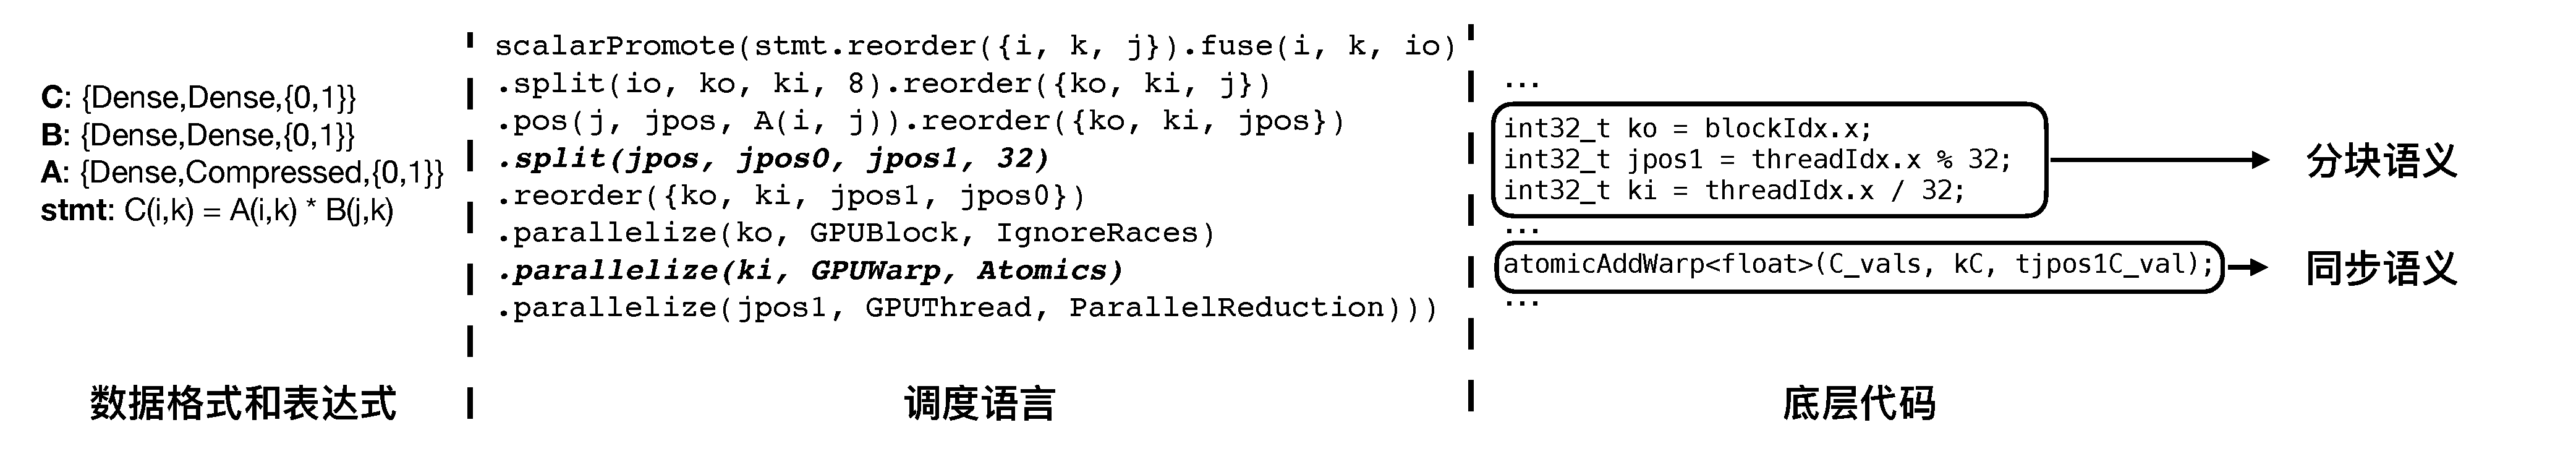
\includegraphics[width=0.99\textwidth]{semantics-cn.pdf}
  \caption{TACO中GPU线程组的分块语义和同步语义}
  \label{fig:sem}
\end{figure}
和TACO不同,TVM只将并行单元绑定在线程和线程块层级,而不会在线程组层面添加含有同步语义的调度指令。它将线程组的大小为32作为一个硬件性质,并用这一性质设置自动调度器中的调度指令参数。同时,它也将线程组作为
一个同步向共享内存或者寄存区中取数据的并行计算单元。

但是,本文提出当前稀疏算子编译器中至少有两个假设可以被突破:线程组分块和同步语义分离。以及同步语义需要可以表达灵活规约。首先,分块语义和同步语义可以被分离,因为分块语义规定了计算顺序,以及根据循环变量恢复原有角标变量
的规则,而同步语义规定的是并行模式,而并行模式规定的是计算顺序如何具体实现。因此二者是两个层面的问题,可以被分离。分块语义和同步语义需要被分离是因为在表~\ref{tab:over-sta-rb}中我们发现,SpMM在RTX 2080上
针对不同稠密矩阵列数,(4, 256, 8, 1/2)都是最佳配置,而这里分块粒度是4,同步粒度是8,二者并不相同。扩展线程组同步语义使其能表达灵活规约后,可以以很低的编程难度提升一类算子的性能。因为添加灵活规约调度指令后,就可以在调度语言层面用同一个调度指令加速加速稀疏稠密混合代数这一类算子。
再比如,SpMM优化空间中$\{<1\,nnz , x\,col>,r\}$需要同步r个线程,每个线程都在寄存器中保存了各自的行标号。因此,线程组规约应该根据行标号的不同,有不同的输出,也就是~\ref{sec:flexible-reduciton}节中的写回线程概念。
在当前稀疏算子编译器中假设只有一个写回线程,但在灵活规约扩展优化空间中写回线程可以有多个。
线程组分快和同步语义分离,和同步语义灵活规约表达不仅需要增加新的底层代码中线程组规约模板函数,也需要将灵活规约计算模式从底层代码传递到顶层调度语言中。这需要新的基本块组织方式,新的控制流和新的用户API。这些技术统称为
灵活规约语义提升技术。
\begin{figure}[h]%
  \centering
  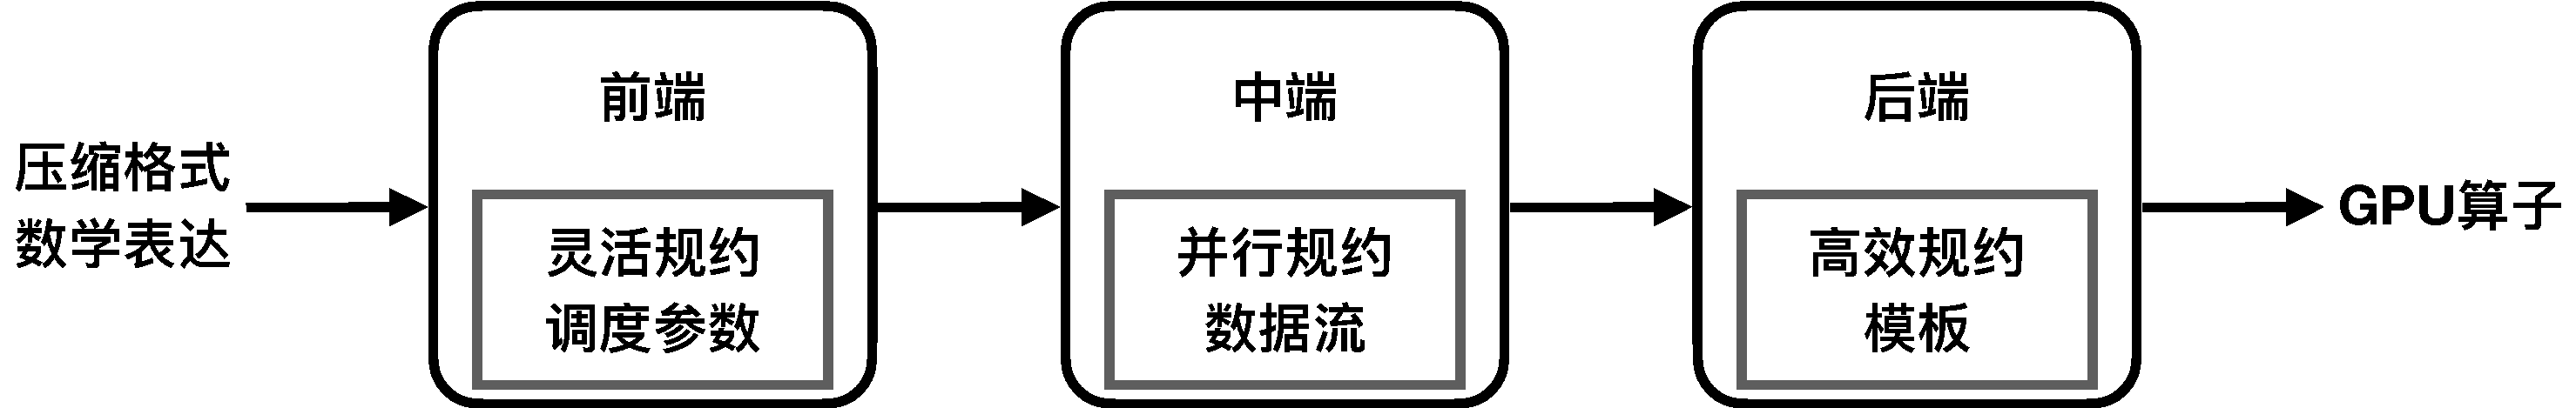
\includegraphics[width=0.99\textwidth]{overview.pdf}
  \caption{编译算法流程图}
  \caption*{圆角方框表示编译器功能模块层次,矩形方框表示本文添加的部分。}
  \label{fig:compiler-overview}
\end{figure}
\section{算法流程}
~\ref{sec:compiler-alg-intro}节提出灵活规约语义提升的两个内涵:线程组分块和同步语义分离,和同步语义灵活规约表达。实现这两个目标需要在前端、中端、后端三方面提出解决方案。具体而言,在前端引入新的并行计算单元抽象,并针对线程组的
分块语义设计新的调度指令。在中端,突破之前串行代码的语义分析逻辑,根据并行规约调整基本块和数据流。在后端,编写高效GPU线程组规约模板,并与中端的IR统一接口,使其执行前端输入的调度策略。以下以TACO编译器为例阐述这三部分编译算法,图
~\ref{fig:compiler-overview}总结了算法流程。
\subsection{前端}
在TACO中,前端提供了\textit{parallelize}接口表示并行计算,它定义为\textit{parallelize(IndexVar i, ParallelUnit pu, OutputRaceStrategy rs)}。这个变换使用并行计算单元$pu$在循环变量$i$上做并行执行。同时输出竞争策略$rs$
描述了在规约时发生的数据竞争。对GPU而言,$pu$可以是线程(GPUThread),线程组(GPUWarp)和线程块(GPUBlock),输出竞争策略$rs$可以是没有竞争(NoRaces),忽略竞争(IgnoreRaces)和原子操作(Atomics)。
为了实现分块和同步语义分离,添加新的并行计算单元(ParallelUnit):GPUGroup,用来描述并行度小于32的线程组并为其添加同步语义,同时取消并行计算单元GPUWarp的同步语义,仅保留分块语义。
具体而言,因为GPUWarp现在只作为分块中外部循环的线程编号,因此使用GPUWarp作为并行计算单元时取消了原子操作的输出竞争策略。同时,在使用GPUWarp时添加新的规约策略(ReductionStrategy)和线程组大小(GroupSize),并去掉输出竞争策略。
规约策略可以指定线程组的规约种类,比如~\ref{sec:flexible-reduciton}节中提到的分段规约和整体规约。GroupSize指定了规约并行度。
\subsection{中端和后端}
因为后端决定了中端的IR变换,同时二者通过IR连接,所以二者放在同一章节介绍。TACO提出一个稀疏张量算子编译器应该尽可能保证只有会产生非零输出的元素才会被计算。但是,在GPU灵活规约中,这一点并一定不成立。TACO的这个非零元素要求是在代码串行执行条件下的最优策略,因为在串行执行下,运算指令越少执行时间越短。
但是在SIMT架构下,规整但是计算量稍大的计算也可能快于计算量小但是不规整的计算。因此,在中端需要添加补零操作。与之搭配的技术成为零扩展。零扩展意味着向稀疏循环理论中添加一些超过边界的规约。这些规约之后会被后端的高效线程组规约模板执行,并且比for循环更快。
\begin{figure}[h]%
  \centering
  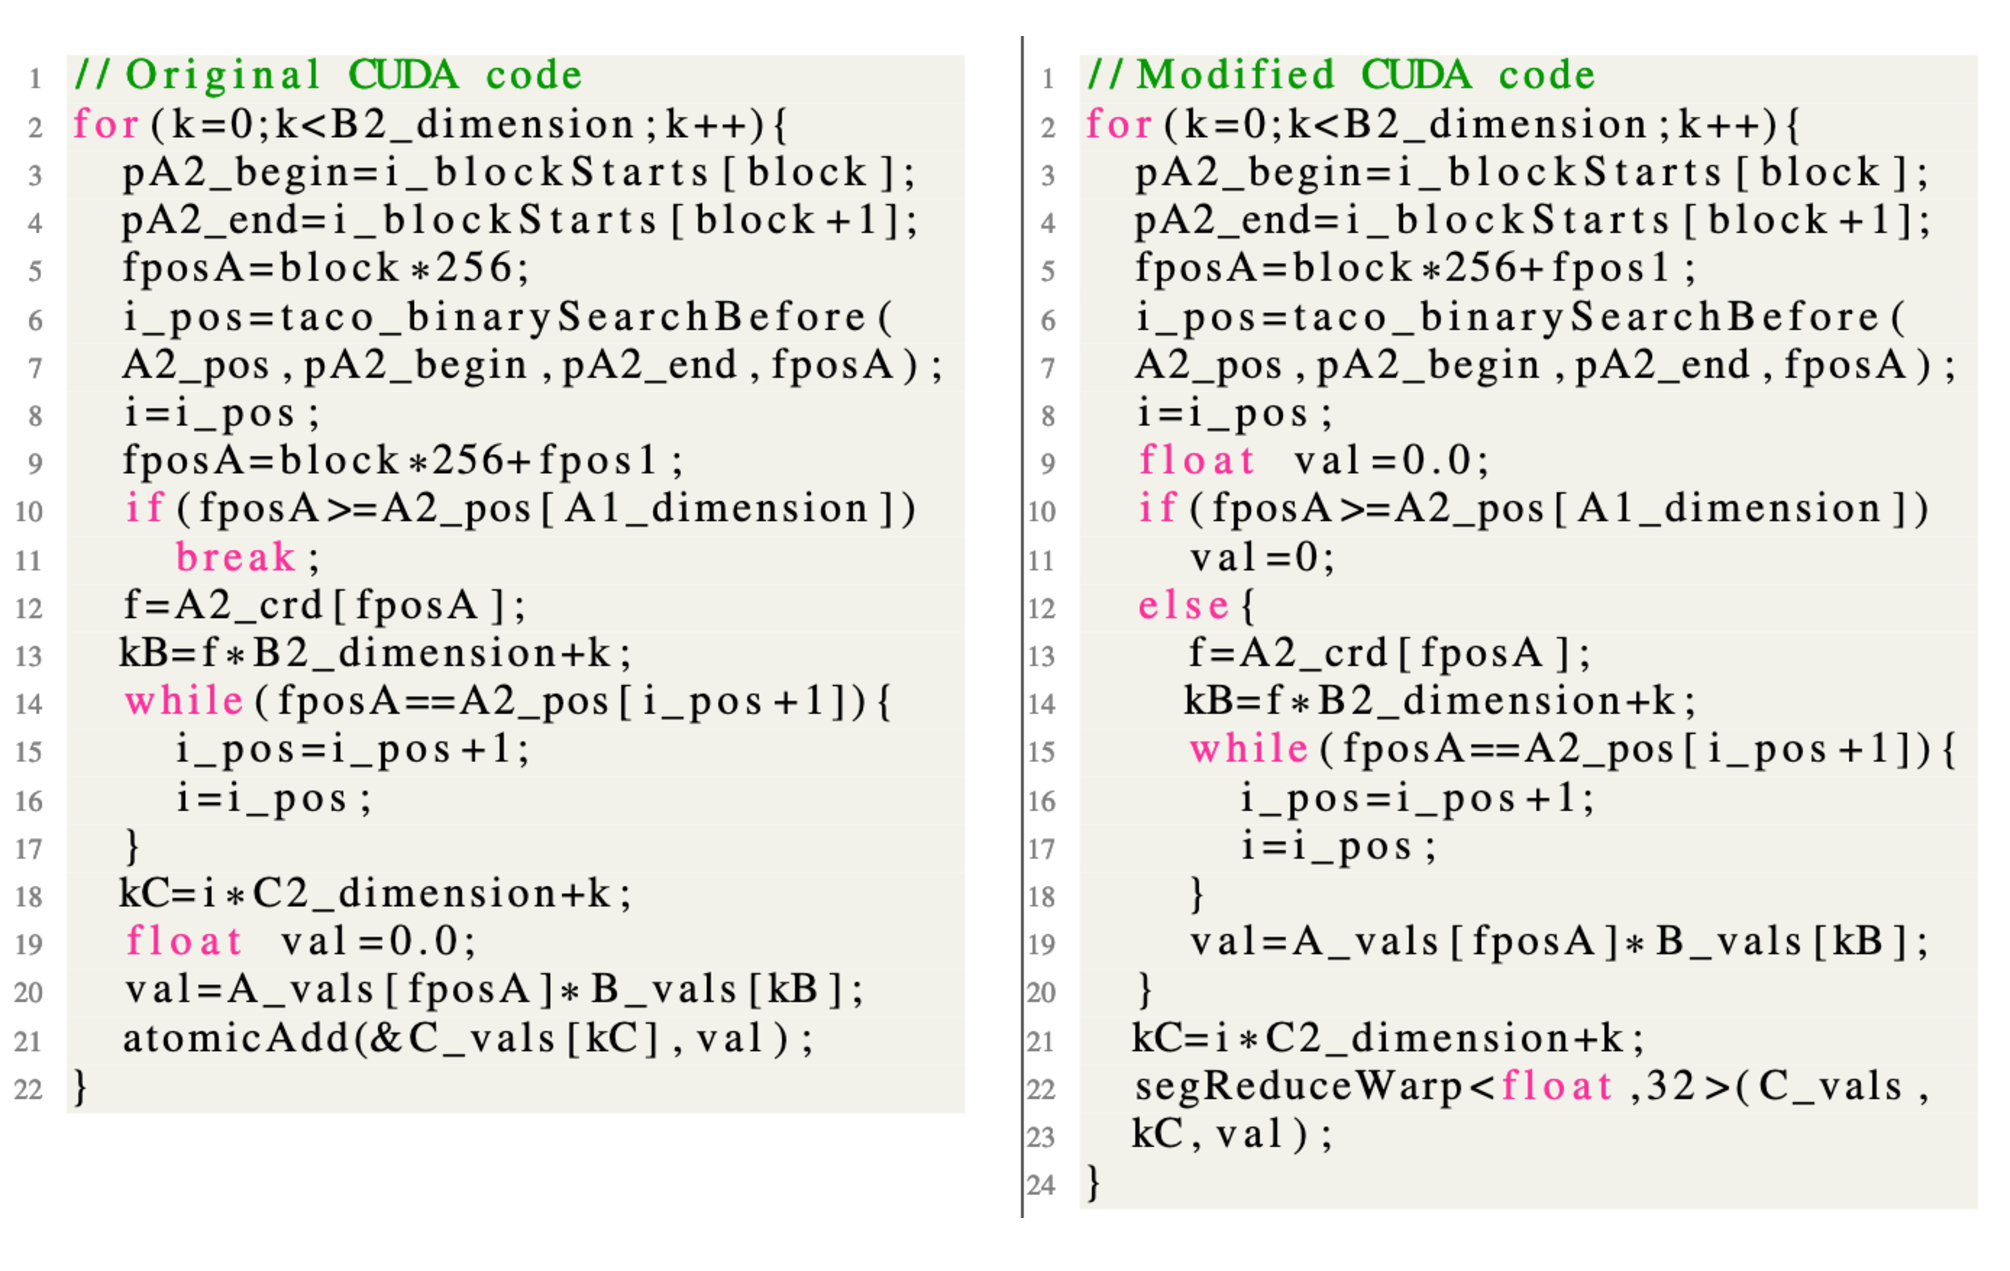
\includegraphics[width=0.99\textwidth]{code.pdf}
  \caption{生成CUDA代码示例}
  \caption*{左侧是修改前编译器生成的代码,右侧是利用灵活规约语义提升添加灵活规约扩展后编译器生成的代码.}\label{fig:code-example}
\end{figure}
图~\ref{fig:code-example}中对比了编译器修改前和修改后生成的代码。右侧代码使用GPUGroup作为并行计算单元,使用分段规约作为规约策略,使用32作为GroupSize,左侧代码使用GPUWarp作为计算单元,原子操作作为输出竞争策略,使用32作为分块粒度。除此之外,他们使用了相同的调度命令。二者有两处不同:标量转移空间,和宏指令。

标量转移空间:TACO假设标量转移空间的声明和赋值在同一个基本块中\cite{kjolstad:2019:workspaces}。这限制了TACO对于稀疏稠密张量计算的表达能力。例如,在$\{<1\,nnz , c\,col>,32\}$中,标量转移空间的赋值发生在属于else的基本块中,
但是标量转移空间的声明发生在和变量转移空间规约相同的上下文中。也就是声明发生在赋值的基本块外。如图~\ref{fig:controlflow}所示,为了实现零扩展,需要改变控制流。添加超过边界后的补零操作,同时将累计额和输出的功能集成到CUDA规约模板中。
\begin{figure}[h]%
  \centering
  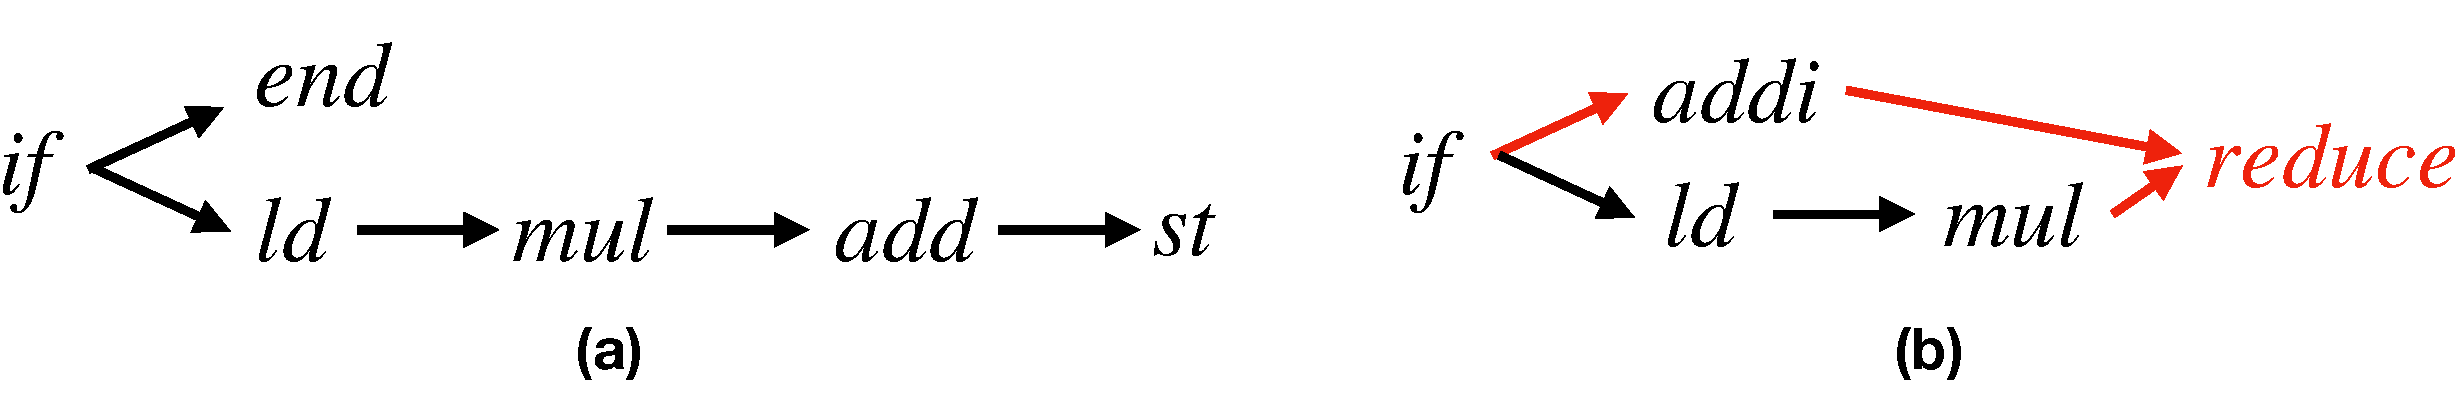
\includegraphics[width=0.99\textwidth]{controlflow.pdf}
  \caption{控制流变化示意图}
  \caption*{图(a)代表修改前的控制流,图(b)代表添加灵活规约语义提升后的控制流。其中if表示进行一个判断,if向上箭头表示条件满足后进入的基本块,向下箭头表示条件不满足进入的基本块。ld表示取数据,mul表示标量乘法,add表示标量加法,st表示存数据。addi表示含有一个常数的标量加法,这里用于实现零扩展。reduce表示一个线程组规约。因为规约中包含累加和存储操作,所以图(b)没有add和st。红色表示新增的操作和执行流。}
  \label{fig:controlflow}
\end{figure}
宏指令:我们希望设计模块化的代码生成系统,这样既利于简化上层IR变换,也利于CUDA指令更新。因为有一些特殊指令不能用于其他架构,所以不适合作为IR,而适合作为模版,其功能可以用上层IR描述,接口上暴露给上层一个简单的函数调用即可。
因此,我们设计了两个新的宏指令\textit{atomicAddGroup$<$T,G$>$(T* array, int idx, T value)}和\textit{segReducWarp$<$T,G$>$(T* array, int idx, T value)}。这两个模板函数的输入是输出向量的起始地址,输出的角标和需要被规约到输出的值。
他们将在G个线程中做规约,这里的G等于GroupSize。在具体实现上,他们会在头文件中声明,然后在最终的CUDA算子代码中作为宏指令被调用。事实上,部分灵活线程组技术来自于CUDA中的合作线程组(cooperaive group)特性。从CUDA11.0开始,CUDA开始支持易用的合作线程组
调用接口\footnote{\url{https://docs.nvidia.com/cuda/cuda-c-programming-guide/index.html\#cooperative-groups}},这使得在底层代码中控制小于32个线程粒度的同步,只需要实例化线程组对象然后调用相关方法。
\section{系统部署}
本节将以SpMM为例介绍灵活规约优化空间扩展在算子编译器中的部署和实现。我们将首先回顾TACO提出的两个SpMM算法,$\{<g\,nnz, c\,col>,1\}$和$\{<x\,row,c\,col >,1\}$。之后我们将使用$\{<\frac{1}{g}\,row, c\,col>,r\}$和$\{<1\,nnz , c\,col>,r\}$这两个例子展示具象角标表示(CIN)的变换过程。
SpMM的数学表达式$C(i,k) = A(i,j) * B(j,k)$。$A$的第一层是稠密格式,第二层是压缩格式。$B$和$C$都是稠密矩阵。$A,B,C$都是行优先存储的。在例子中我们会将$p,g,N,c$以字母形式填入CIN中来展示他们和CIN参数的运算关系。但是真实的CIN不会有没有确定的数值。
\subsection{已有优化空间}
当前TACO可以支持灵活规约扩展优化空间中的两类算法,$\{<g\,nnz, c\,col>,1\}$和$\{<x\,row,c\,col >,1\}$。因为其默认同步粒度是32,同时采用线程组整体规约,所以他们不需要同步语义,而只在分块语义层面进行性能调优。两种算法各自的CIN如图~\ref{fig:CIN-1}和图~\ref{fig:CIN-2}所示
它们强制要求同步粒度是1,因此限制了规约的优化空间。针对$\{<g\,nnz, c\,col>,1\}$,我们采用~\ref{sec:spcomp}节介绍的角标表示重写类生层如图~\ref{fig:CIN-1}所示的CIN。在~\cite{senanayake:2020:scheduling}中,采用$N=128,g=16,c=4,p=512$进行性能实验。
针对$\{<x\,row,c\,col >,1\}$,我们直接使用TACO命令行工具即可生成,在~\cite{senanayake:2020:scheduling}中,采用$N=128,g=1,c=4,p=512$进行性能实验。这两种算法都只用到了GPUWarp的分块语义。
\begin{figure}[h]%
  \centering
  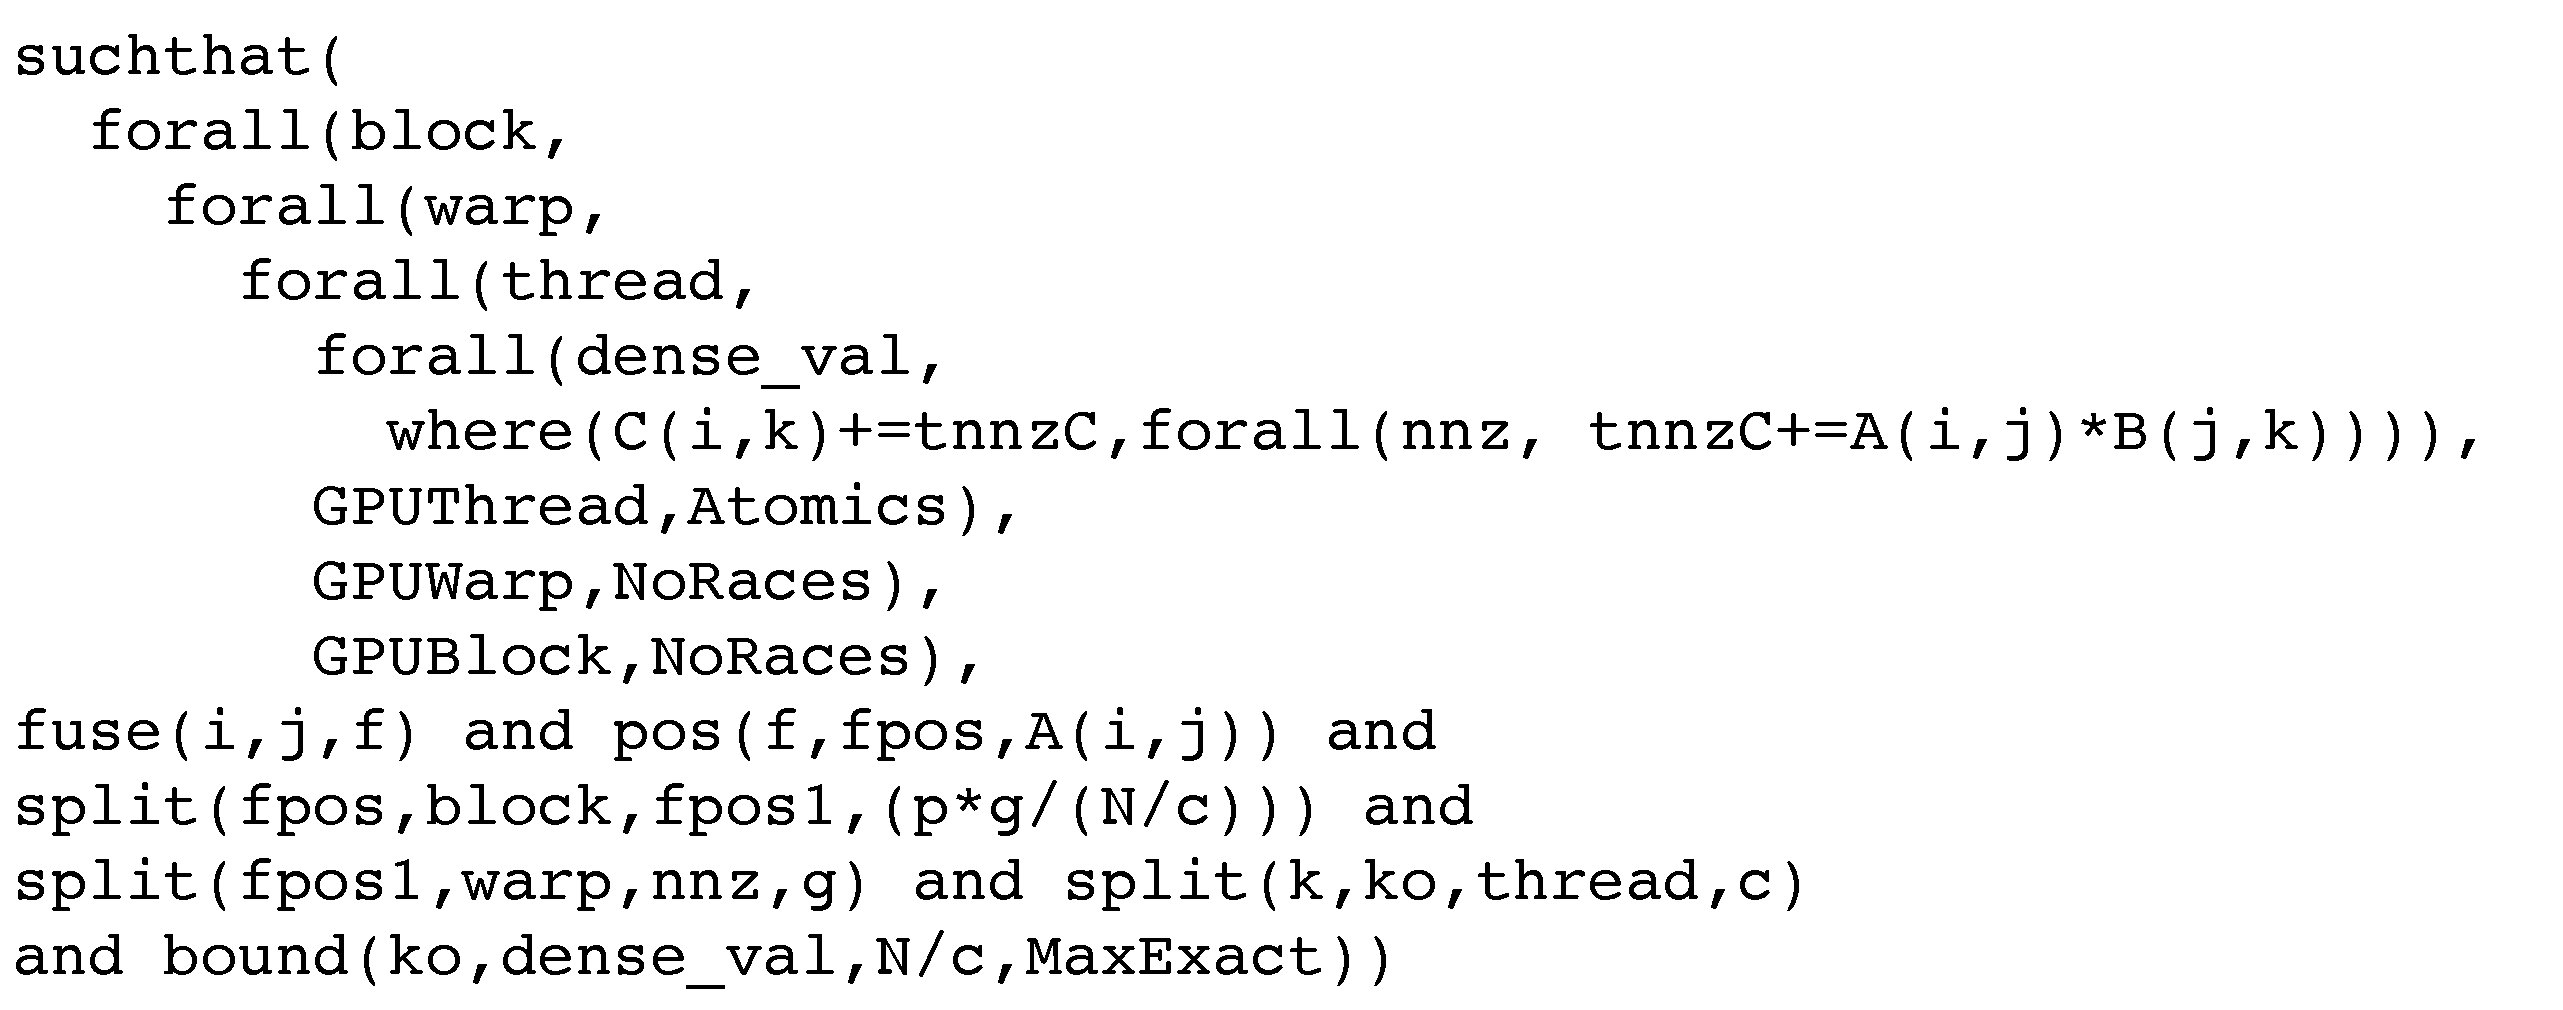
\includegraphics[width=0.99\textwidth]{CIN-1.pdf}
  \caption{$\{<g\,nnz, c\,col>,1\}$的CIN}\label{fig:CIN-1}
\end{figure}
\begin{figure}[h]%
  \centering
  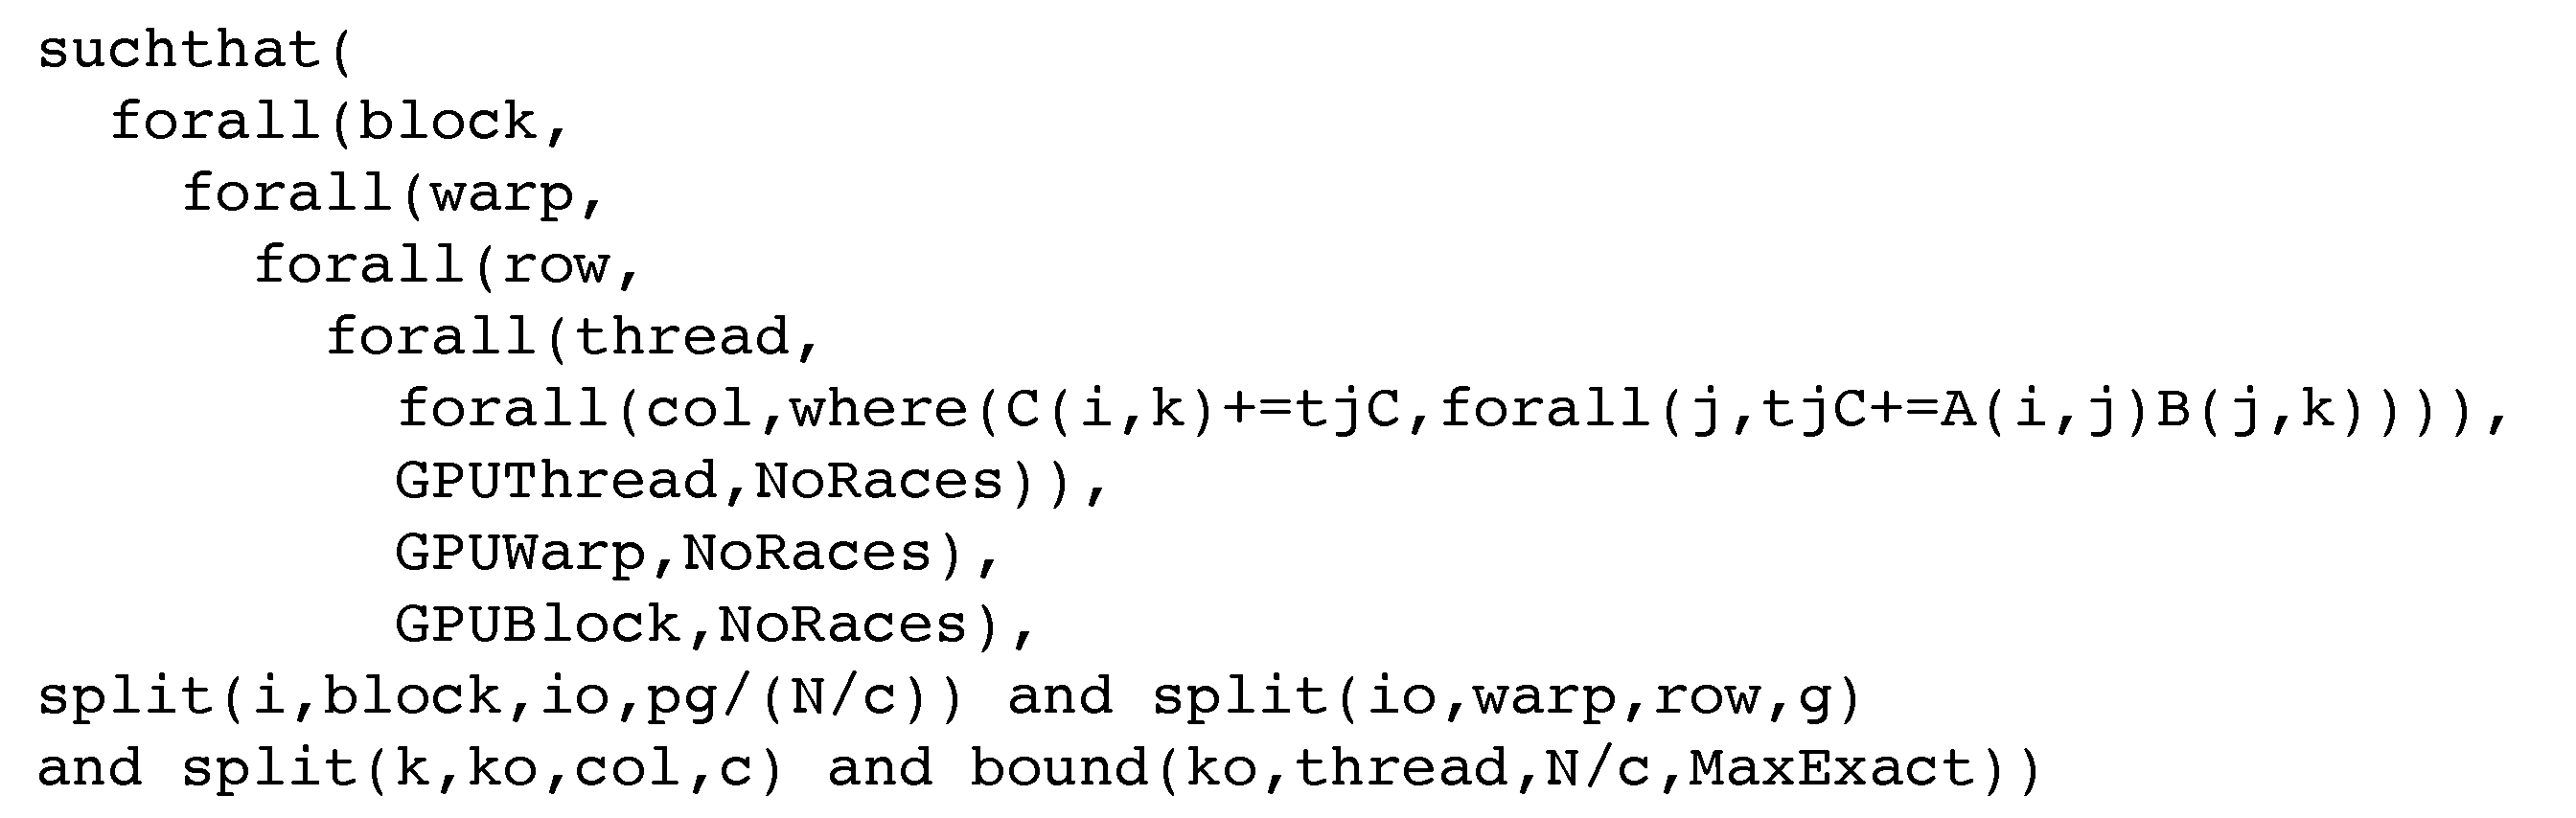
\includegraphics[width=0.99\textwidth]{CIN-2.pdf}
  \caption{$\{<x\,row,c\,col >,1\}$的CIN}\label{fig:CIN-2}
\end{figure}
\subsection{扩展优化空间}\label{sec:comp-space}
将灵活规约扩展优化空间中的$\{<\frac{1}{g}\,row, c\,col>,r\}$和$\{<1\,nnz , c\,col>,r\}$引入稀疏算子编译器可以提升工作负载均衡。如图~\ref{fig:CIN-3}和图~\ref{fig:CIN-4}所示,这两种算法提供了变换线程组大小和规约策略的功能。用户可以针对非零元和行数的性能调优。
\begin{figure}[h]%
  \centering
  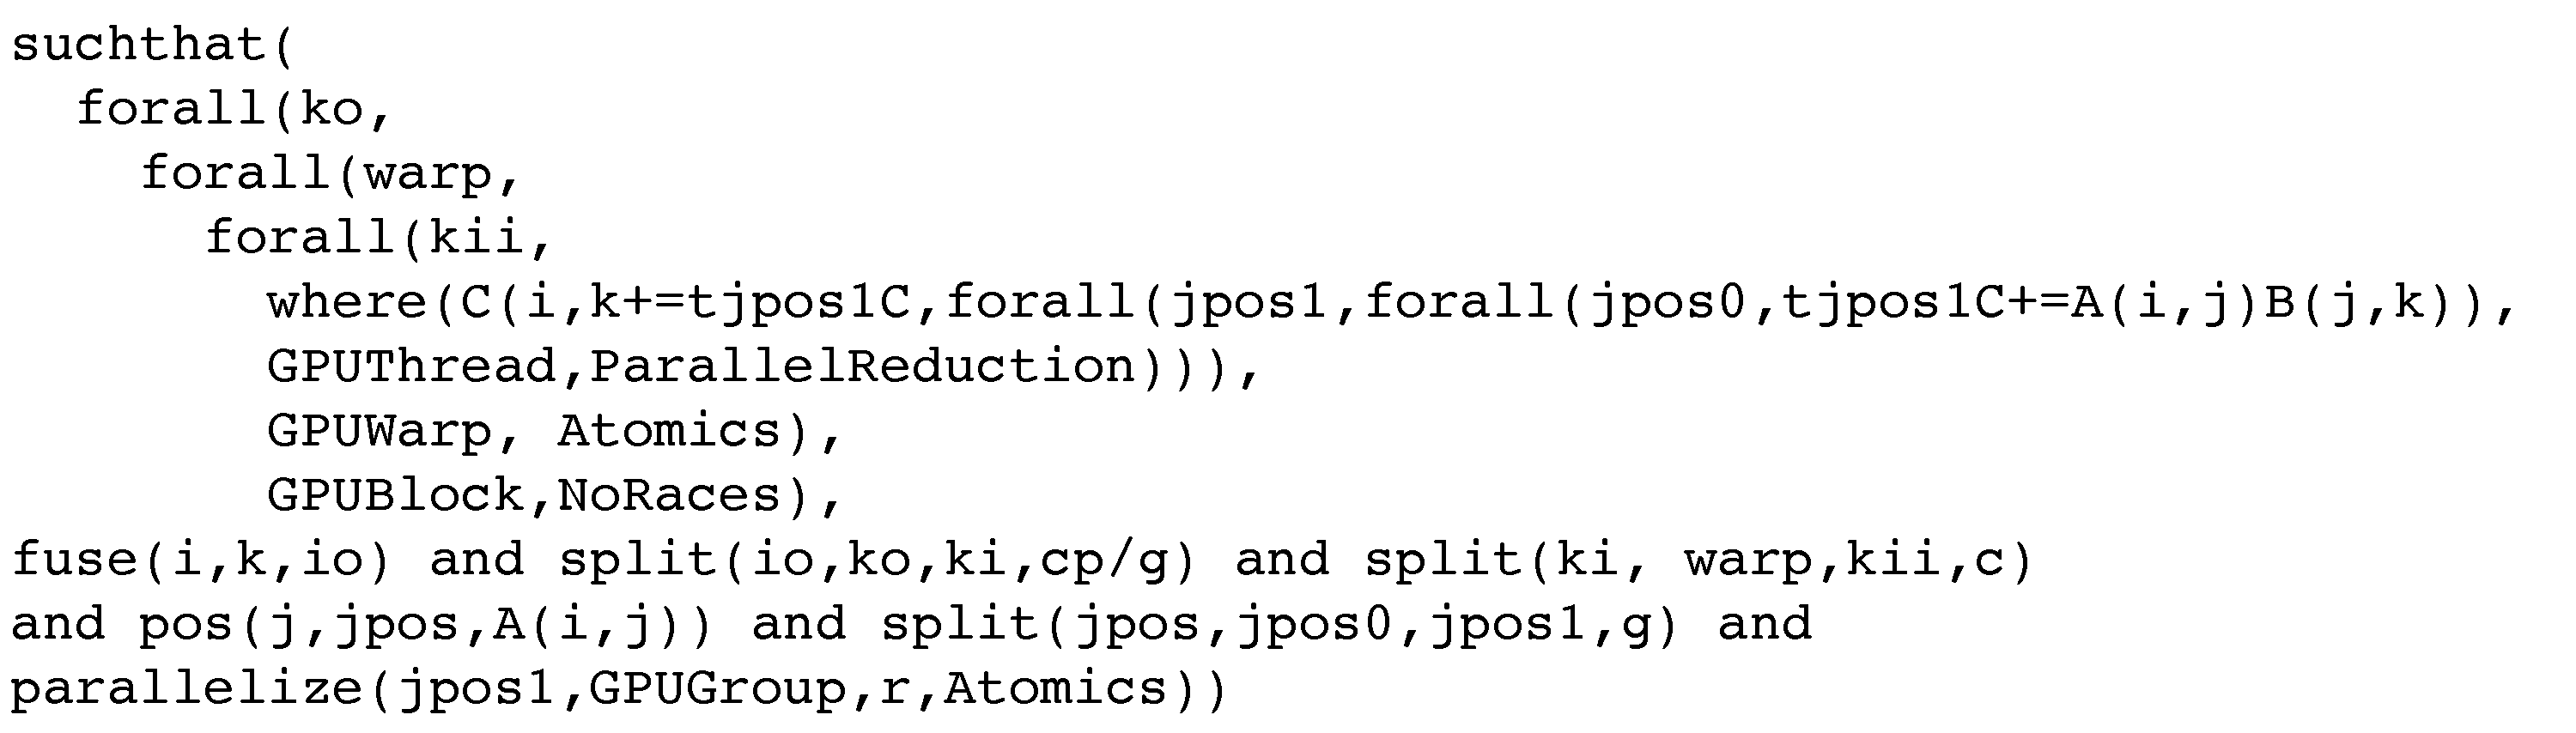
\includegraphics[width=0.99\textwidth]{CIN-3.pdf}
  \caption{$\{<\frac{1}{g}\,row, c\,col>,r\}$的CIN}\label{fig:CIN-3}
\end{figure}
\begin{figure}[h]%
  \centering
  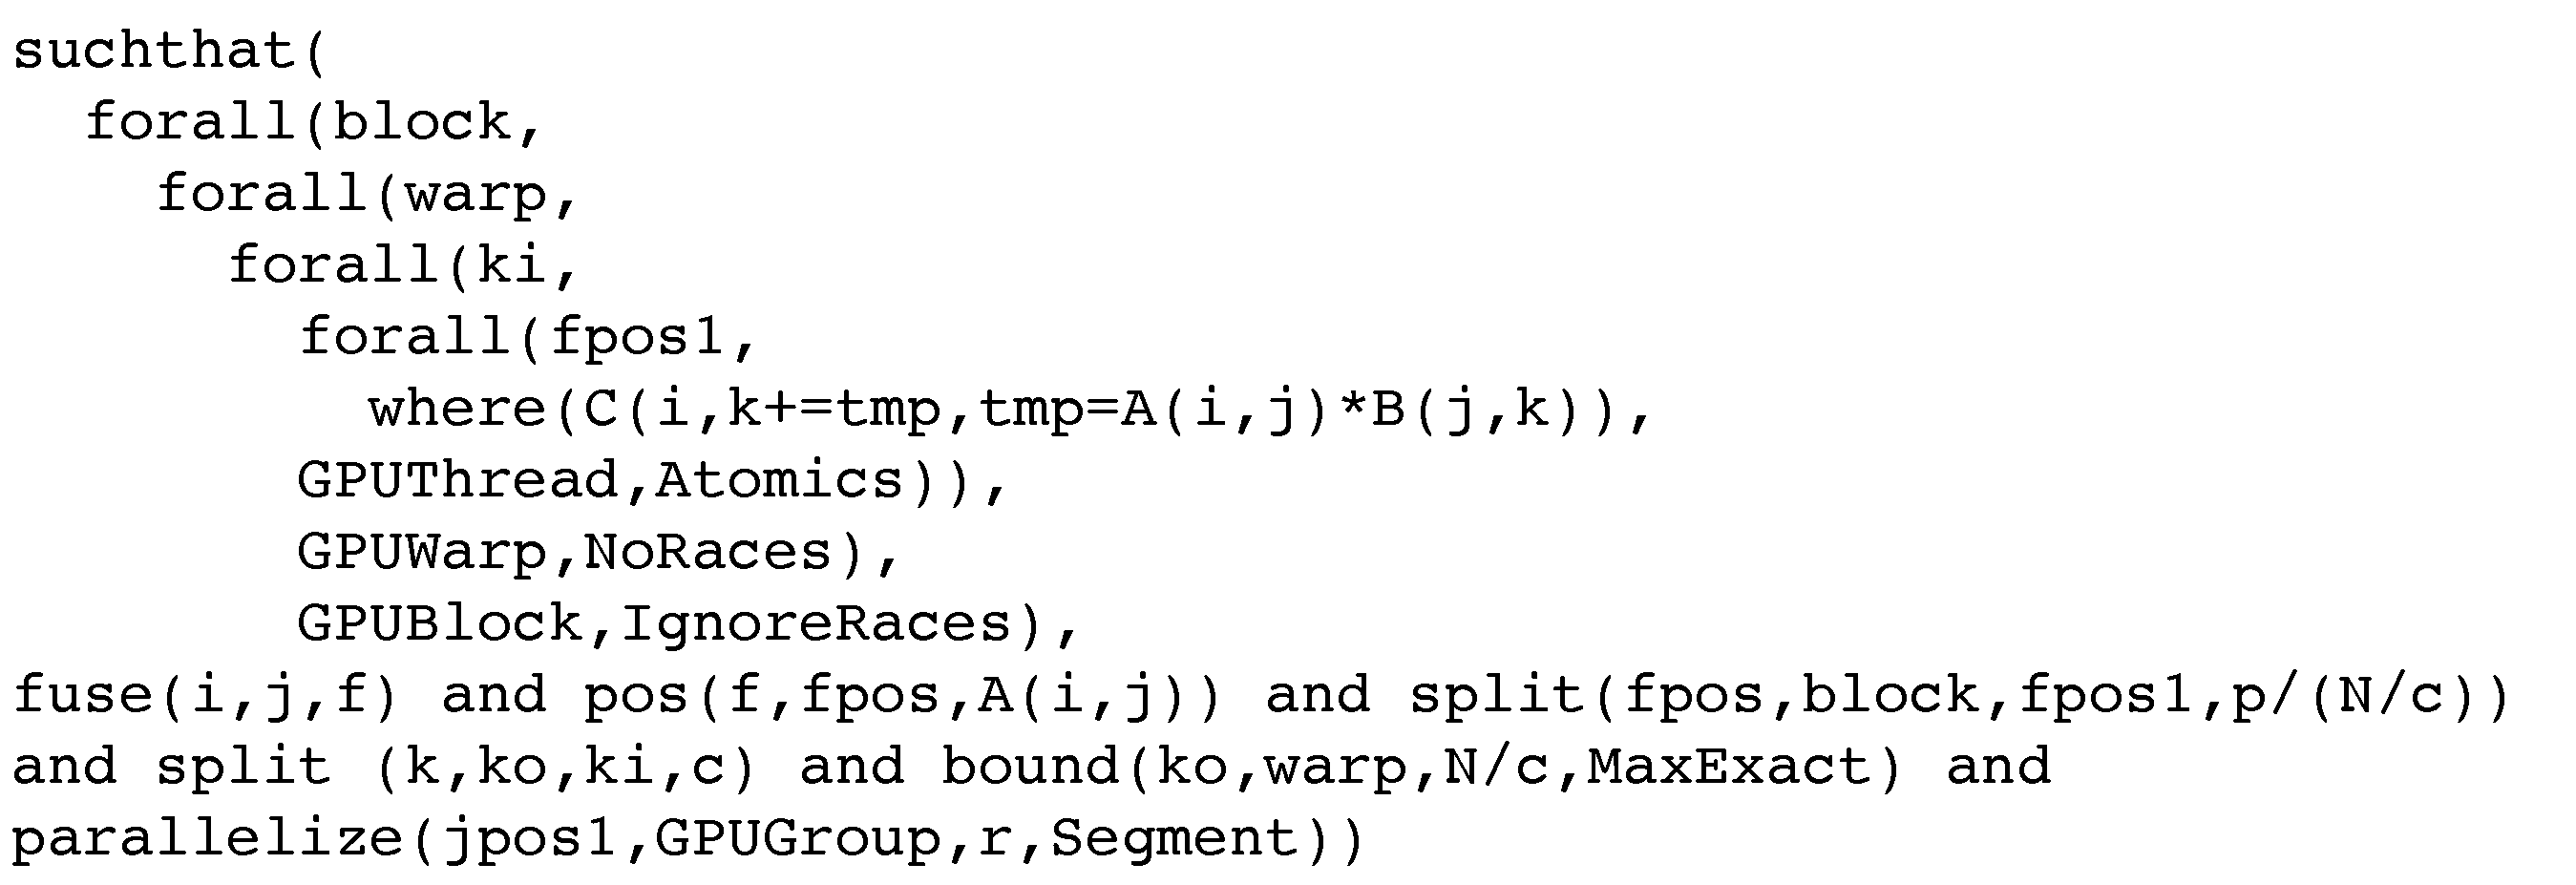
\includegraphics[width=0.99\textwidth]{CIN-4.pdf}
  \caption{$\{<1\,nnz , c\,col>,r\}$的CIN}\label{fig:CIN-4}
\end{figure}
实际上TACO可以支持$g=32, r=32$的$\{<\frac{1}{g}\,row, c\,col>,r\}$算法,但是TACO不能支持其他参数的该种算法。GPUGroup被完成规约的循环变量所限制。原本生成的宏指令\textit{atomicAddWarp$<$Type$>$}被替换成\textit{atomicAddGroup$<$Type, G$>$}来处理更细粒度的线程同步。
图~\ref{fig:CIN-4}展示的$\{<1\,nnz , c\,col>,r\}$算法在原本的TACO中没有被支持。我们将原本发射的\textit{atomicAdd}替换成\textit{segReduceGroup$<$Type,G$>$},分段规约就在新的宏指令中完成。标量转移空间的中端变换也被转换成可以执行分段规约的数据流。

\section{实验结果}
实验环境和~\ref{sec:exp-env}节中相同。本节实验用于证明灵活规约语义提升技术可以提高稀疏算子编译器的优化空间表达能力,并提高编译器生成算子的质量。在实验中未明确指出时稠密矩阵列数N默认为4。
\subsection{灵活规约粒度和静态规约粒度对比}
我们使用$\{<\frac{1}{g}\,row, c\,col>,r\}$来展示引入灵活规约粒度后带来的算子性能提升。如~\ref{sec:comp-space}节提到的,当前TACO只支持$g=32, r=32$。因此我们控制$g$为与TACO相同的32,并改变$r$。在表~\ref{tab:comp-flexgra}中展示了$r=8$和$r=4$可以给原有算子带来超过2倍的性能提升。
其中A相对于B的后验性能提升表示,当A比B的性能更好时,记录加速比;当A的性能不如B时,加速比记为1。这种统计方式展示了添加自动性能调优器后灵活规约带来的性能提升上限。
\begin{table}
  \centering
  \caption{灵活规约粒度对比静态规约粒度性能提升}
  \begin{tabular}{llllll}
  \toprule
  硬件平台 &  $r=8$  & $r=8$后验 & $r=4$  & $r=4$后验\\
  \midrule
  RTX 2080    & 2.451   & 2.478 & 2.456 & 2.483 \\
  RTX 3090    & 2.236   & 2.284  & 2.259 & 2.307 \\
  Tesla V100    & 2.086  & 2.143  & 2.094 & 2.150 \\
  \bottomrule
  \end{tabular}
  \label{tab:comp-flexgra}
\end{table}
\subsection{灵活规约策略和单一规约策略对比}
我们使用$\{<1\,nnz , c\,col>,r\}$来展示灵活规约策略带来的性能提升。本节以分段规约和整体规约为例,因为他们有不同的数据类别(非零元与行),因此我们控制$c$和$r$相同,并将$\{<1\,nnz , c\,col>,r\}$与改变$g$得到的最优的$\{<\frac{1}{g}\,row, c\,col>,r\}$的性能。
这一实验只在RTX 3090上完成,此处记录的是后验加速比。在表~\ref{tab:comp-flexstr}中展示了分段规约可以比之前TACO中采用的整体规约加速1.3倍。受限于GPU提供的最大线程组大小为32,所以$r$只能是$1,2,4,8,16,32$。因此,在实际使用中用户可以尝试使用这些数字对$r$进行性能调优。
\begin{table}
  \centering
  \caption{灵活规约策略对比单一规约策略性能提升}
  \begin{tabular}{llllll}
  \toprule
  c &  $r=4$  & $r=8$ & $r=16$  & $r=32$\\
  \midrule
  1   & 1.008   & 1.025  & 1.085 & 1.272 \\
  2    & 1.019   & 1.045  & 1.102 & 1.291 \\
  4   & 1.063   & 1.095  & 1.205 & 1.381 \\
  \bottomrule
  \end{tabular}
  \label{tab:comp-flexstr}
\end{table}
\subsection{灵活规约与优化前编译器对比}
在这一实验中,我们对比TACO的原始SpMM算法$\{<g\,nnz, c\,col>,1\}$和$\{<x\,row,c\,col >,1\}$,以及灵活规约语义提升新增的$\{<\frac{1}{g}\,row, c\,col>,r\}$和$\{<1\,nnz , c\,col>,r\}$。
各种算法中的$g,c,x,$和$r$参数被赋予合理的值并进行性能调优。我们记录了每种算法在每个数据集上的后验最佳性能。从表~\ref{tab:comp-all}中我们可以得出灵活规约可以生成1.1倍到1.2倍更快的算子。同时,我们也
测试了不同稠密矩阵列数下的实际性能提升(即非后验性能)。如图~\ref{fig:comp-tables}所示,可以发现稠密矩阵列数越小,灵活规约的优势越大。
\begin{table}
  \centering
  \caption{灵活规约与优化前编译器生成算子后验性能对比}
  \begin{tabular}{lllll}
  \toprule
  & RTX 3090  & RTX 2080 & Tesla V100 \\
  \midrule
  加速比   & 1.191   & 1.098  & 1.223\\
  \bottomrule
  \end{tabular}
  \label{tab:comp-all}
\end{table}
\begin{figure}[h]%
  \centering
  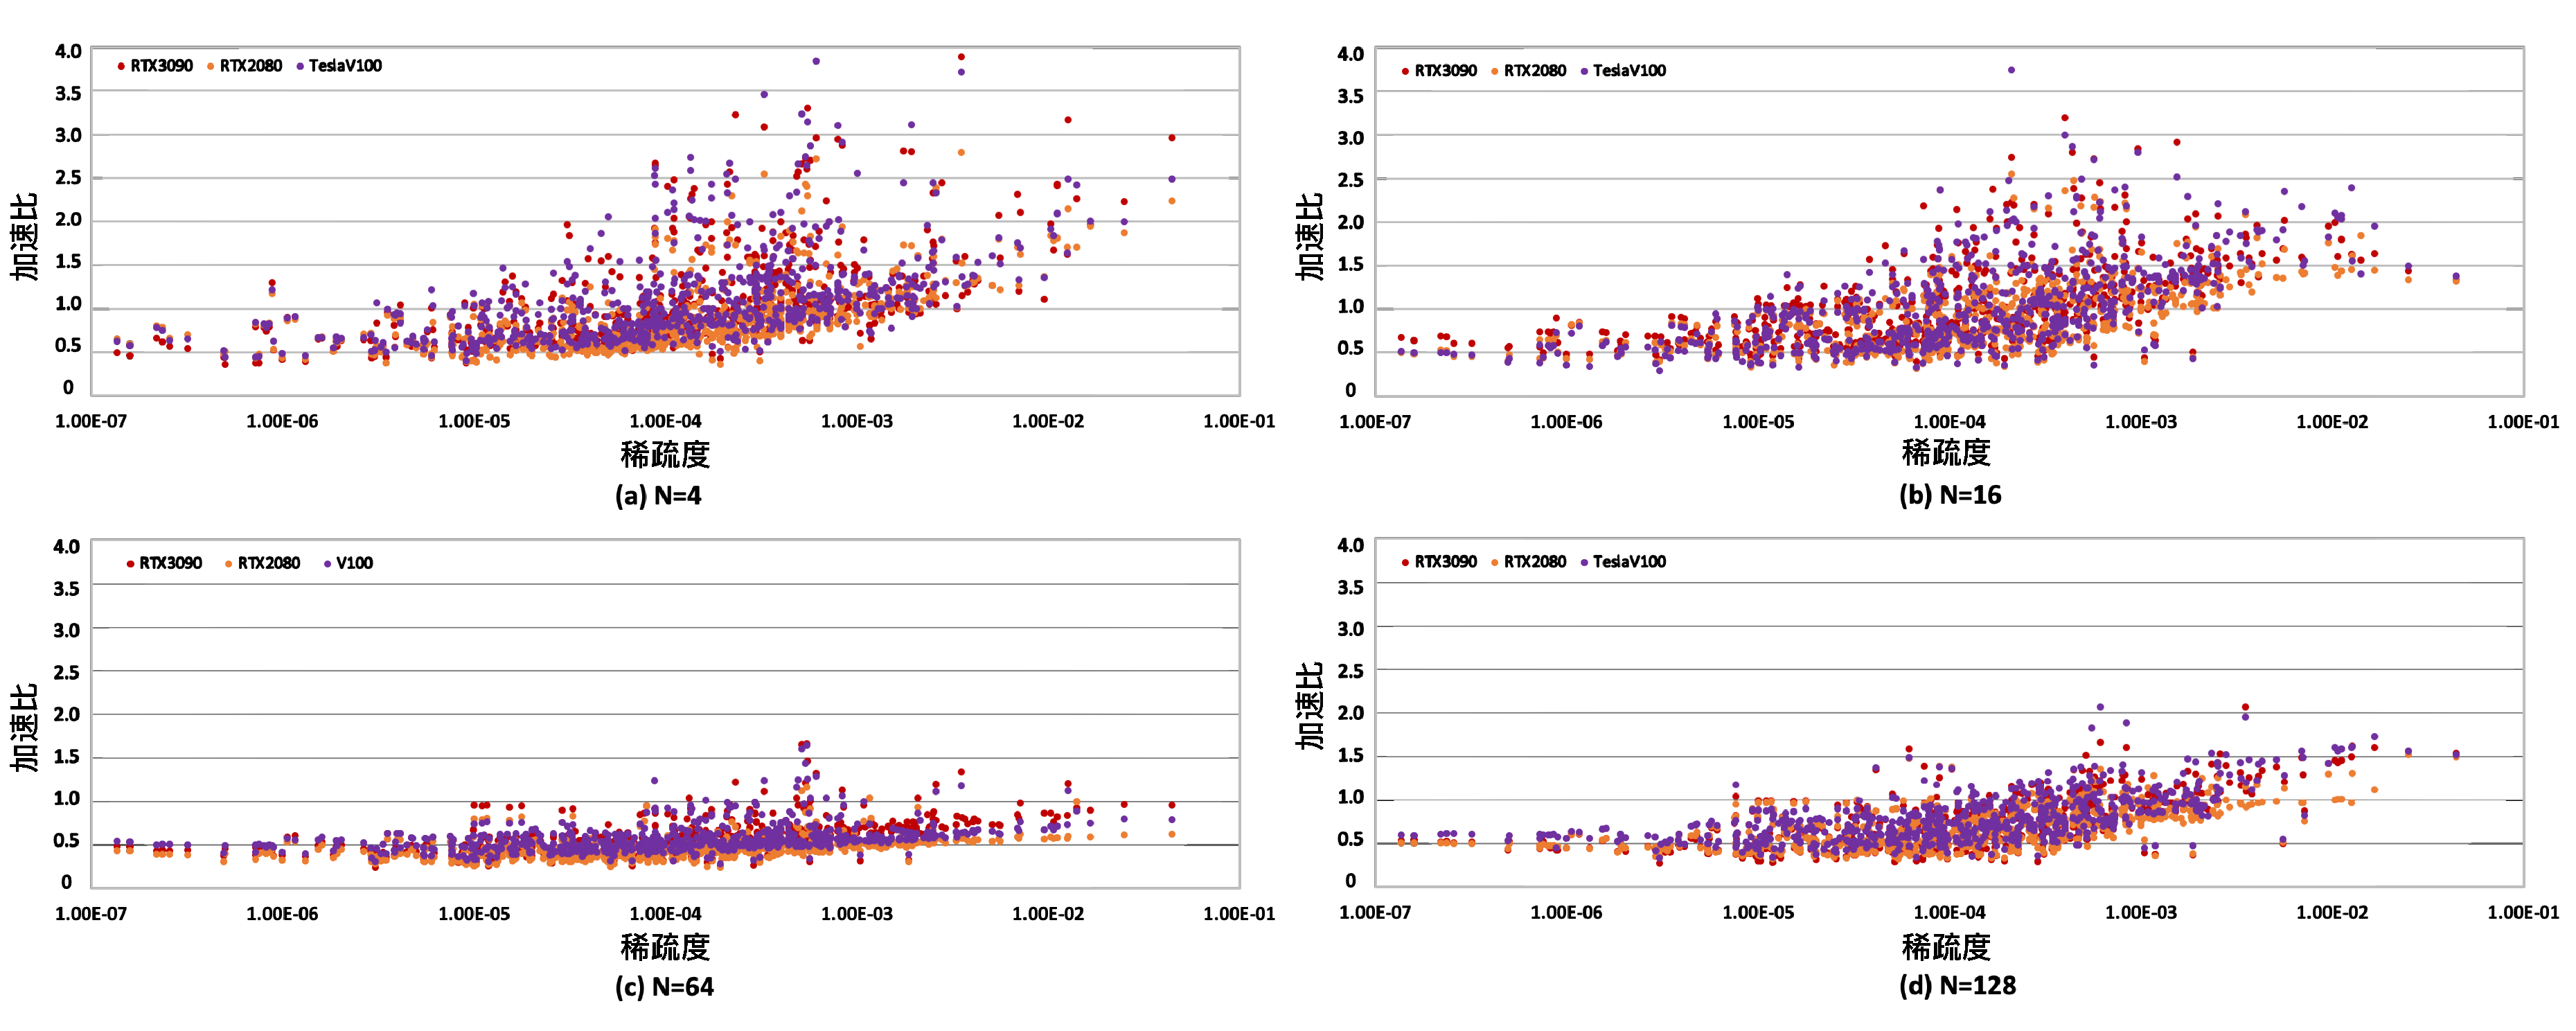
\includegraphics[width=0.99\textwidth]{new_tables-cn.pdf}
  \caption{不同稠密矩阵列数下灵活规约与优化前编译器生成算子性能对比}
  \caption*{稀疏度定义为稀疏矩阵中非零元个数除以行数和列数的乘积。}
  \label{fig:comp-tables}
\end{figure}
\subsection{灵活规约优化泛化性}
优化泛化性是指除了自身的优化对象,一种优化技术可以加速其他算子。在~\ref{sec:reduction-core}节中分析了优化规约就可以加速稀疏稠密混合代数。本节以MTTKRP为例,通过实验表明灵活规约的优化泛化性。采用和~\cite{senanayake:2020:scheduling}中相同的
调度指令,只是规约部分改成灵活规约。表~\ref{tab:tensor-info}展示了测试所用三维稀疏张量的基本信息。高维稀疏张量数据较为稀缺,这里选取的8个三维稀疏张量是常用的开源稀疏张量数据。图~\ref{fig:comp-mttkrp}展示了MTTKRP在freebase\_music和freebase\_sampled这两个数据集上可以获得最高2.7倍的性能提升。
\begin{table}
  \centering
  \caption{MTTKRP测试张量信息}
  \begin{tabular}{lllll}
  \toprule
  张量名称& 第一维  & 第二维 & 第三维 & 稀疏度 \\
  \midrule
  1998DARPA   & 22K  & 22K & 23K  & 2.37E-09\\
  amazon-reviews   & 4.8M  & 1.7M & 1.8M  & 1.13E-10\\
  delicious-3d   & 0.53M  & 17M & 2.5M  & 6.14E-12\\
  flickr-3d   & 0.32M  & 28M & 1.6M  & 7.8E-12\\
  freebase\_music   & 23M  & 23M & 0.17K  & 1.10E-09\\
  freebase\_sampled   & 39M  & 39M & 0.53K  & 1.73E-10\\
  nell-2   & 12K  & 9.2K & 29K  & 9.05E-13\\
  nell-1   & 0.32M  & 28M & 1.6M  & 9.05E-13\\
  \bottomrule
  \end{tabular}
  \label{tab:tensor-info}
\end{table}
\begin{figure}[h]%
  \centering
  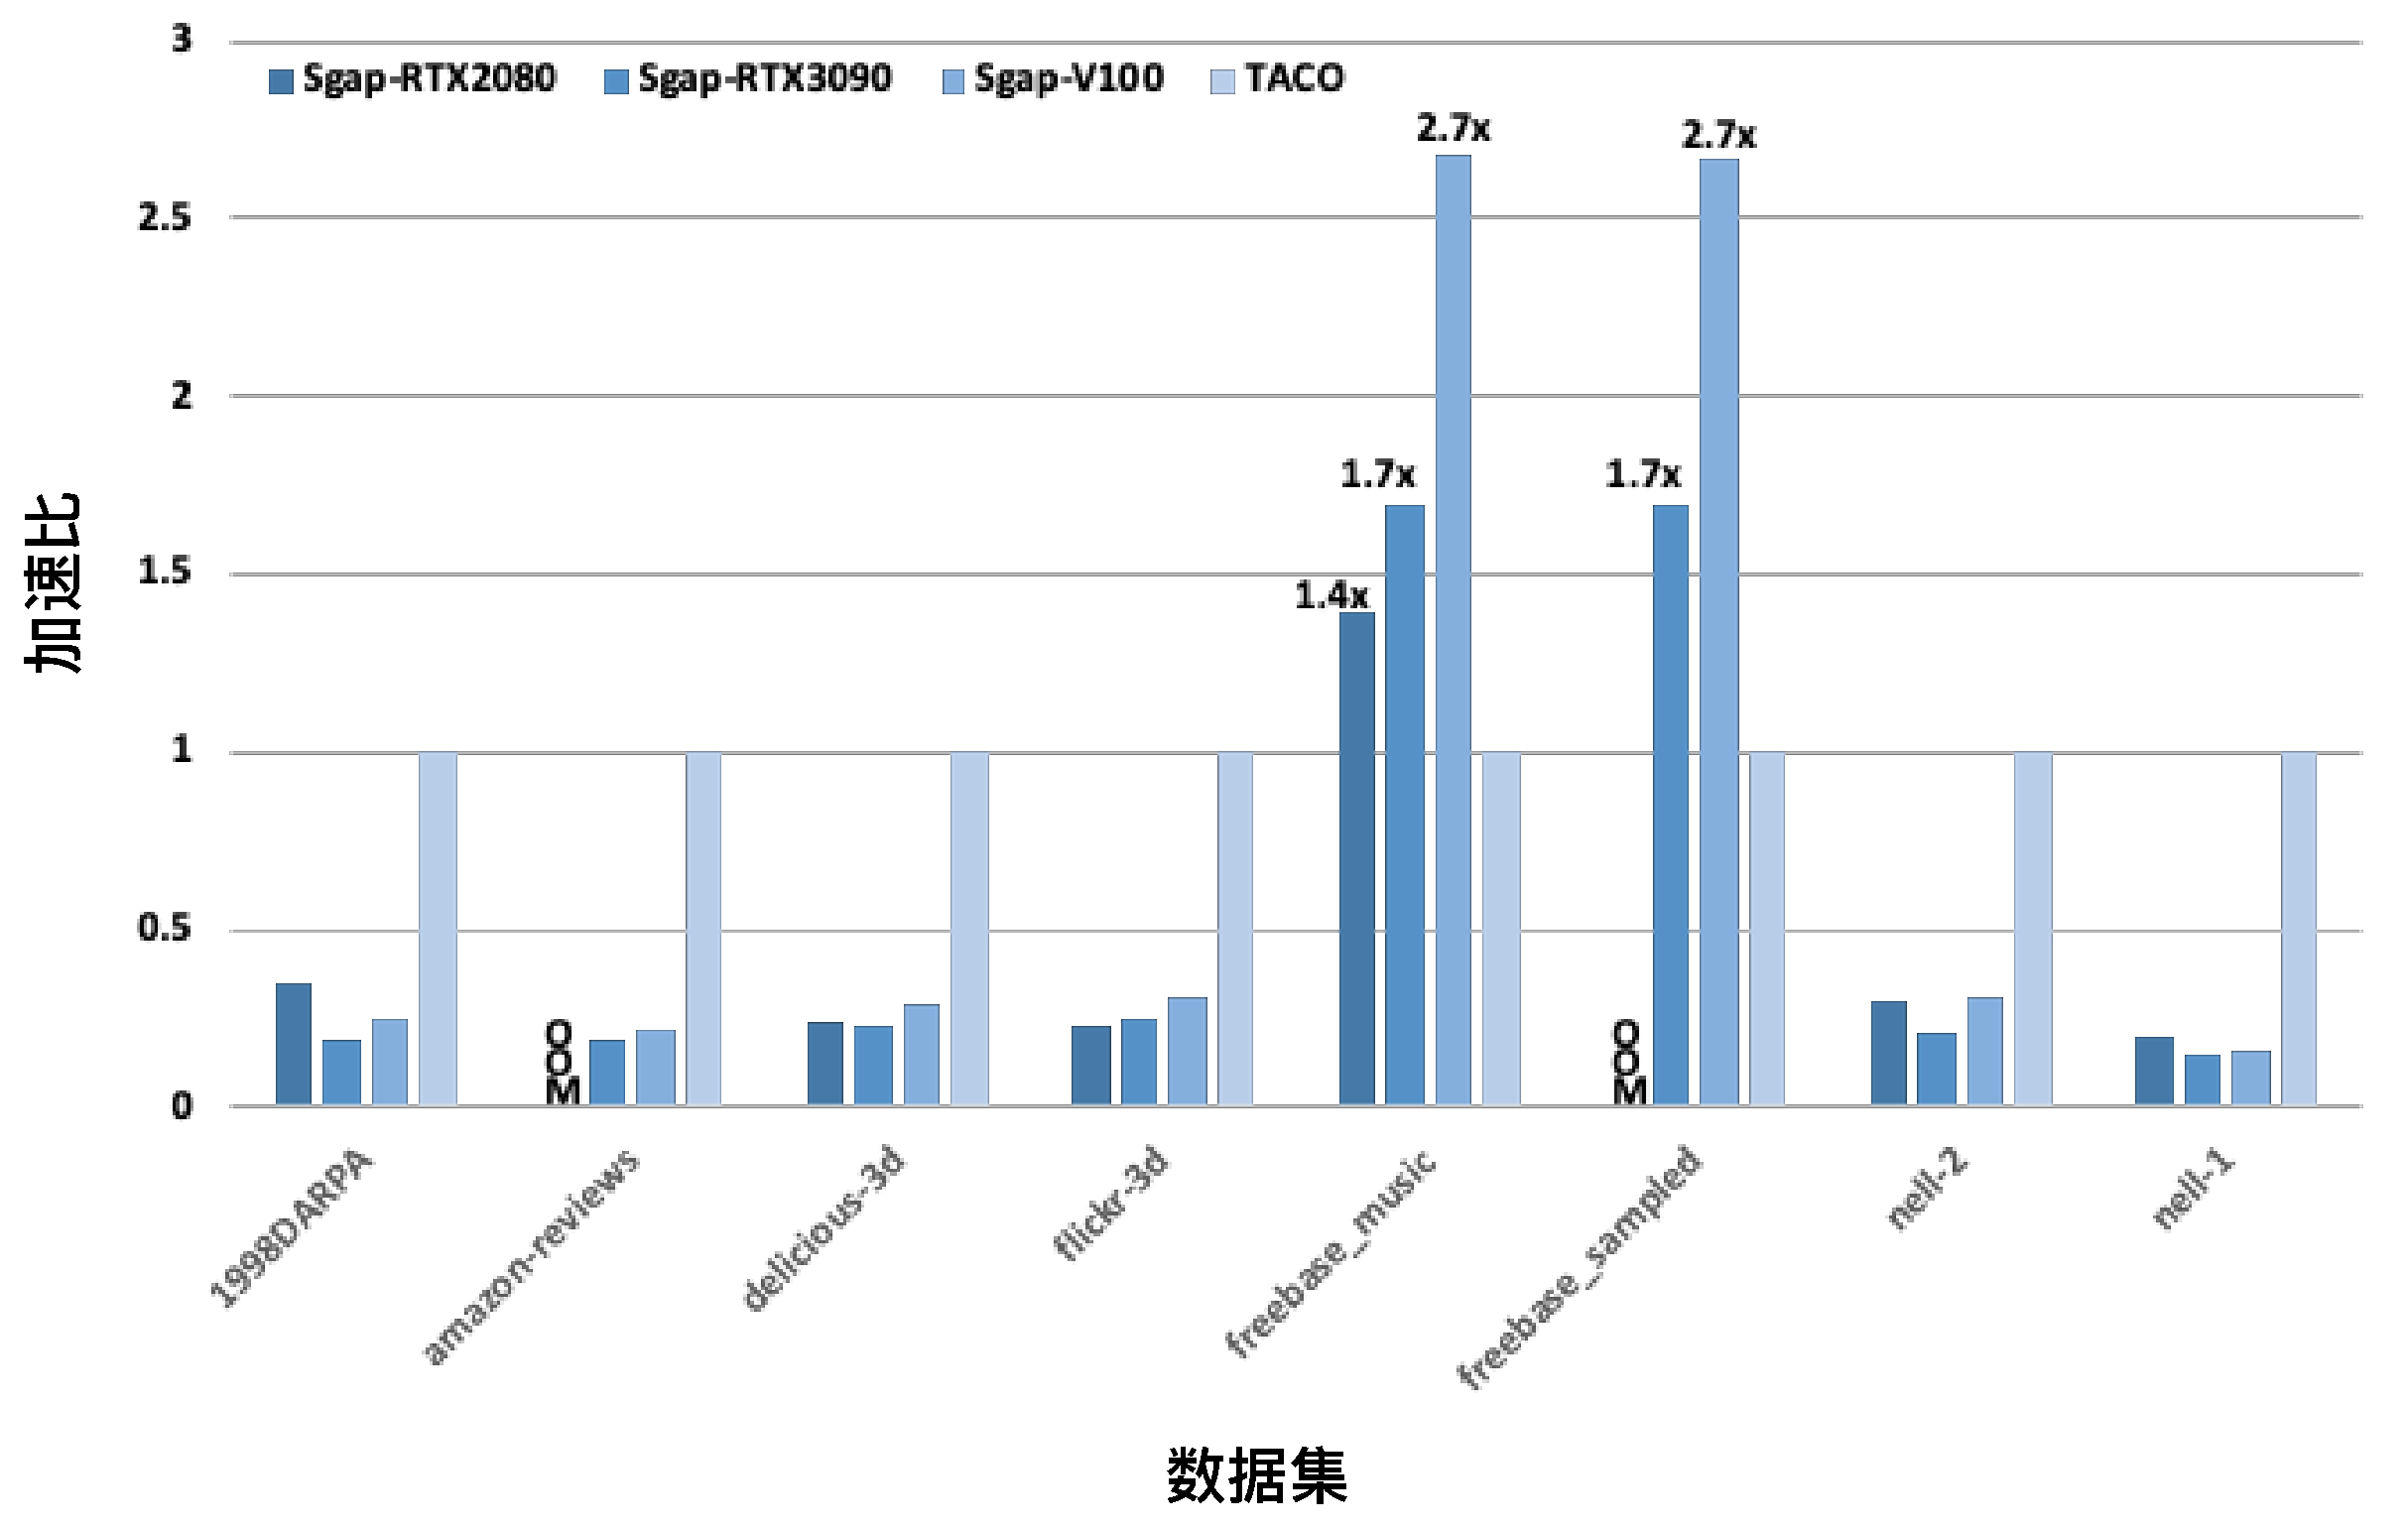
\includegraphics[width=0.99\textwidth]{mttkrp.pdf}
  \caption{MTTKRP在不同数据集下灵活规约和编译器原有算法生成算子性能对比}
  \caption*{图中OOM(Out-Of-Memory)表示算子运行过程中显存溢出。}
  \label{fig:comp-mttkrp}
\end{figure}
% !TeX root = ../thuthesis-example.tex

\chapter{总结}
\thusetup{
  cite-style = super,
}
\section{本文结论}
本文依照优化技术归纳、同类算子演绎和编译算法设计的思路展示了针对稀疏稠密混合代数在单指令多线程架构上灵活规约优化空间扩展的编译算法设计,在算子性能、优化技术泛化性和开发效率方面取得了提升,并为更广泛的通用稀疏张量计算编译算法设计提出了可行的研究方法。
针对稀疏稠密混合代数在SIMT架构上优化不充分和开发难度高的问题,本文提出了灵活规约优化技术和灵活规约语义提升技术。

灵活规约优化技术包含灵活规约粒度和规约策略,该技术扩展了当前的基于原子并行模型的稀疏稠密混合代数优化空间。同时本文从张量形式和表形式两个角度论证了在原理上可以将性能提升泛化至所有稀疏稠密混合代数。
实验结果显示,在稀疏稠密矩阵向量乘算子上灵活规约取得了比最优开源算子库1.6到2.7倍性能提升。

基于扩展后的优化空间,本文将灵活规约纳入稀疏迭代模型,并提出灵活规约语义提升技术,在稀疏算子编译器前端添加灵活规约调度参数;中端添加并行规约数据流;后端添加高效规约模板。
该技术使得用户可以通过简单调度指令针对任意稀疏稠密混合代数进行灵活规约扩展优化空间的性能调优。实验结果显示,该技术将原有稀疏算子编译器生成的SpMM性能提升平均1.2倍,最高3.8倍;MTTKRP算子最高提升2.7倍。


\section{相关工作}
下面首先回顾算子编译器产生动机,指出其学术研究价值和产业应用潜力。张量编译器指为高效张量计算设计的编译器\cite{halide,kjolstad:2017:taco}。常见的张量编译器输入为描述张量运算的高级语言。
深度学习编译器\cite{tvm,rammer}的核心之一也是张量编译器,因为当前机器学习算法的核心算子为张量运算。常见深度学习编译器输入为神经网络计算图描述语言和参数文件。
二者输出均为硬件平台特定低级语言。与张量编译器不同,深度学习编译器同时还包含计算图优化,算子融合等技术。因为二者技术类似,所以下面统称算子编译器。
深度学习框架\cite{tensorflow,pytorch}与算子编译器不同。框架常以扩展包形式嵌入到其他常用高级语言(如Python, C++),不直接输出硬件算子,而是调用硬件平台提供的算子库(如英伟达GPU的cuDNN算子库\cite{cuDNN})。
算子编译器较算子库相比优势为开发成本低和灵活度高。在实际生产中,针对特定硬件的高效深度学习算子库开发长达几个月甚至几年,很难满足专用硬件量产需求和算法迭代速度\cite{Heron}。
而编译器可以通过计算元语模板和优化空间自动探索技术,在几小时甚至几分钟内生成和算子库性能相当的算子\cite{Roller}。同时,因为编译器可以做代码级别变换,所以很方便做算子融合。
算子融合技术可以加速深度学习算法推理速度,最高可达10倍左右\cite{DNNFusion}。而算子库的功能在开发时就已确定,无法做细粒度的算子融合\cite{Graphene}。
因此,有越来越多学者开始关注这一领域\cite{PET,Tiramisu,Checkmate},硬件提供商也在积极研发算子编译器技术,比如英伟达的Triton\cite{Triton},和华为的AKG\cite{AKG}。

\section{未来工作}
上节分析了算子编译器的发展动机,下面基于三个典型问题阐释算子编译器的核心优化技术,并指出未来可能的研究和应用方向。

第一个问题:算子编译器能否表达手工算子优化的技术?硬件架构特性规定了所有可能的算子优化技术。以GPU为例,double-buffer技术基于GPU的shared memory-register file两层级存储架构\cite{double-buffer};并行规约技术基于GPU的CUDA Core中线程同步架构\cite{parallel-reduction};
tiling技术基于DRAM的coalesce访存架构\cite{coalesce};data-layout在寄存器中的排布要适应Tensor Core的指令特殊规定\cite{DynamicNM}。因此,如果算子编译器
生成的算子想要逼近甚至超过算子库性能,算子编译器就需要可以表达尽可能多的手工算子优化技术。这是算子编译器的基本问题,因为如果无法表达算子优化技术,无论怎么微调参数都难以超过手工算子性能。
换句话讲,算子编译器需要随着硬件架构的演进不断扩展优化空间。因此,只要应用需求推动硬件架构持续创新,算子编译器领域就将大概率出现更多新技术。

已有较多工作基于此思路。比如ALCOP\cite{ALCOP}基于Tensor Core架构将“多级访存-计算流水线”算子技术引入算子编译器,生成的算子较TVM1.23倍的平均加速;
TensorIR\cite{TensorIR}基于Tensor Core架构引入硬件特殊加速的特定形状矩阵乘法,生成的算子较TVM提升了最多7.5倍。 本文也是沿着这个思路。
首先通过分析GPU架构特征,提出灵活规约同步粒度这一稀疏稠密混合算子优化技术。手工验证该技术有效后,通过在后端设计算子模版,中端调整计算流图,前端设计调度API,最终实现用户仅添加一条调度指令就可以享受到算子性能提升。

第二个问题:如何设计中间表示(intermediate representation,简称IR)?IR是连接用户代码和机器码的中间组件\cite{IR},它是编译器表达手工算子优化技术的手段。如果没有IR,即用户代码直接经过多次变换生成机器码,会有两个问题:部署成本高和维护复杂。机器的ISA更改则必须重写编译器,由于前端后端强耦合,更改编译器代码会产生副作用\cite{LLVM}。
因此,算子编译器也需要IR。算子编译器中有三类常见IR:一是顶层抽象编译器支持的操作,二是底层抽象硬件架构,三是中层连接性的IR。底层IR为顶层IR提供计算平台基础,顶层IR为底层IR提供应用场景,中层IR作为编译变换的载体连接底层和顶层IR。

从硬件角度设计底层IR比如,在TVM\cite{tvm}中,GPU的并行计算单元被抽象为二维blockIdx和二维threadIdx;而在Roller\cite{Roller}中单个计算单元的能力被抽象为load, compute, store,GPU则被抽象为大量相同的该计算单元;也可以借助MLIR提供的层次化编译变换提供GPU Tensor Core的硬件抽象\cite{mlir-tc}。
从应用角度设计顶层IR比如,CoRA\cite{CoRA}针对不规则稠密矩阵应用设计IR来更高效地规则化计算和融合算子;SparseTIR\cite{SparseTIR}针对稀疏张量计算设计IR来表示数据格式融合和高效混合计算。
当然,也可以先从应用角度设计顶层IR,然后直接将顶层IR中的关键操作设置为底层IR,根据底层IR设计新的硬件架构。比如,SAM\cite{SAM}抽象出稀疏张量运算的9种核心操作,并为稀疏张量数据流加速器提供了直接的硬件模块映射。

第三个问题:算子编译器算子生成效率?由于算子编译器较算子库的一大优势是开发成本低,因此如何更快生成好算子是一个重要的研究问题。这一问题包含两方面:快速判断一个算子的质量(即在实际硬件上运行的速度)和快速生成优质算子。
算子质量判断有两种主流方向。一种是基于搜索得到算子的实际性能历史记录学习得到的机器学习模型,另一种是基于架构特征的近似解析模型。机器学习模型的优势是算法设计和硬件无关,容易迁移;但劣势是需要积累实测的历史数据,搜索时间较长且可解释性差\cite{AutoTVM,Ansor,AMOS}。
解析模型的优势是不需要实测历史记录,可解释性强,但劣势是和架构相关,且需要基于一定假设才能得到近似,容易出现估计偏差\cite{GNNAdvisor,Roller,ALCOP}。
快速生成优质算子常见算法是基于给定元语集合的遗传算法和基于手写模板的快速参数搜索算法。遗传算法的优势是可以探索人工设计没有考虑到的元语组合,劣势是搜索空间稀疏,难以快速搜索到优质算子\cite{Hidet}。
基于手写模板的参数搜索算法优势是可以较快探索局部优化空间,劣势是优化空间受限\cite{Auto-Halide}。

由于稀疏计算复杂性,其优化空间构建仍是开放问题。与稠密计算不同,稀疏计算涉及坐标空间和位置空间变换,而稠密计算一直在坐标空间,这进一步加剧了优化空间的稀疏性\cite{senanayake:2020:scheduling}。
同时稀疏计算任务规模在运行前不可知,而稠密计算可以在运行前分析输入数据并做优化,这对算子编译器运行时优化提出了更大的挑战\cite{Dynamic-tiling}。
因此,当前提升稀疏算子编译器算子生成效率的研究仍处于基于手写模板的阶段。比如TACO自动调度\cite{ahrens:2022:autoscheduling}基于最小化冗余计算的原理提出了构建渐进复杂度意义下最优算子的原则,
WACO\cite{WACO}基于TACO\cite{kjolstad:2017:taco}提供的元语,为稀疏稠密混合代数设计了算子模板,离线构造优化空间,运行时根据输入数据特征搜索最优解。

总的来说,算子开发的目标是更高性能和更高迭代效率,相关技术发展有三大趋势:自动化,结构化和智能化,如图~\ref{fig:future}所示。自动化是指将已经确定的代码写法固化为模板,由程序自动生成。比如本文编译算法的宏指令设计就是将灵活规约固化为模板,有编译器中端自动调用。在实际应用中,英伟达采用模板编程开发了高效线性代数库CUTLASS\cite{CUTLASS}。
该种方式最直接,但是不灵活。结构化是指将已有的优化技术通过中间表示泛化至一类算子。比如本文编译算法的标量转移空间设计就是将灵活规约通过LLIR应用到所有稀疏稠密混合代数中。在实际应用中,Halide\cite{halide},TVM\cite{tvm}和TACO\cite{kjolstad:2017:taco}都采用了该种技术。该种技术一定程度上降低了优化技巧泛化成本,但是优化空间仍然
限制在人工经验中。智能化是指利用基础模型\cite{Bommasani2021FoundationModels}学习优化技术直接生成算子。这种技术难点是构建反馈闭环,将算子建模为基础模型的序列化输入,以及人工经验的合理嵌入。该种方案可以突破人工经验,迈向算子极致性能优化。
\begin{figure}
  \centering
  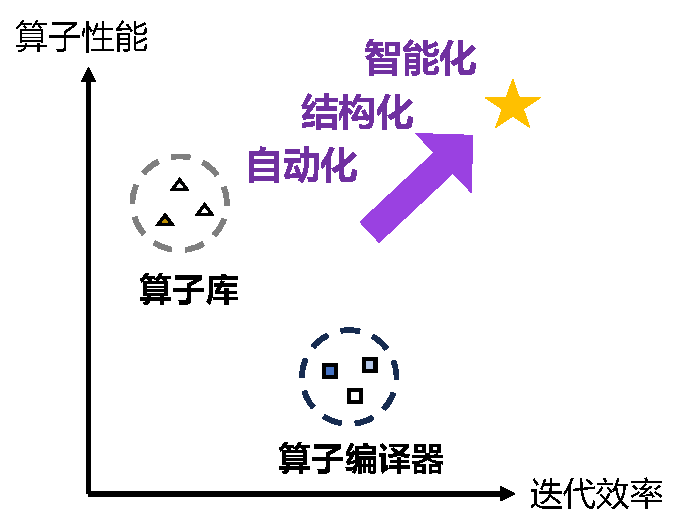
\includegraphics[width=0.6\linewidth]{future.pdf}
  \caption{算子优化技术发展趋势}
  \label{fig:future}
\end{figure}

% 其他部分
\backmatter

\listoffigures           % 插图清单
\listoftables            % 附表清单

% 参考文献
\bibliography{ref/refs}  % 参考文献使用 BibTeX 编译
% \printbibliography       % 参考文献使用 BibLaTeX 编译



% 致谢
% !TeX root = ../thuthesis-example.tex

\begin{acknowledgements}
  感谢汪玉教授和上海交通大学戴国浩教授的悉心指导。汪玉老师和戴国浩老师对待学术研究充满好奇、追求极致的态度让我终身受益。老师们的言传身教也让我不断开拓眼界、提升自我。
  感谢斯坦福大学Fredrik Kjolstad教授的精心指导。Fredrik严谨清晰的治学风格和对于关键问题的精彩点拨让我受益匪浅。本文的编译算法部分基于其TACO系列工作完成。
  感谢加州大学尔湾分校的黄思陶教授,阿伯丁大学的温源教授和曼彻斯特大学的Pavlos Petoumenos教授对于本工作的指导和帮助。本文的最初想法产生于与老师们的讨论。
  感谢NICSEFC实验室稀疏计算小组的同事对我的帮助。本文的算子加速部分基于小组对于GPU稀疏算子加速的技术积累进行改进。
  特别地,感谢爸爸,妈妈和姐姐对于我生活和情感上的支持,和对于我人生追求的支持与鼓励。
  最后,感谢所有关心和帮助过我的朋友们。
\end{acknowledgements}


% 声明
% \statement
% 将签字扫描后的声明文件 scan-statement.pdf 替换原始页面
% \statement[file=scan-statement.pdf]
% 本科生编译生成的声明页默认不加页脚,插入扫描版时再补上;
% 研究生编译生成时有页眉页脚,插入扫描版时不再重复。
% 也可以手动控制是否加页眉页脚
% \statement[page-style=empty]
% \statement[file=scan-statement.pdf, page-style=plain]

% 附录
% 本科生需要将附录放到声明之后,个人简历之前
\appendix
% \input{data/appendix-survey}       % 本科生:外文资料的调研阅读报告
% !TeX root = ../thuthesis-example.tex

\begin{translation}
\label{cha:translation}

\title{张量代数编译转移空间\cite{kjolstad:2019:workspaces}}
\maketitle

\tableofcontents

\section{摘要}

本文展示了如何扩展稀疏张量代数编译器以引入称为转移空间的临时张量,以避免低效的稀疏数据结构访问。我们为张量运算开发了一种称为具体索引符号的中间表示法 (IR),
它指定子计算何时发生以及它们的存储位置。然后,我们将描述此IR中的转移空间转换、如何以编程方式调用它以及如何将 IR 编译为稀疏代码。
最后,我们展示了如何使用该变换来优化稀疏张量算子,包括稀疏矩阵乘法、稀疏张量加法和矩阵化张量乘以Khatri-Rao积(MTTKRP)。我们的结果表明,
转移空间转换使这些算子的性能与手动优化的实现相当。例如,我们将具有密集输出的 MTTKRP 的性能提高了高达 35\%,
并能够生成稀疏矩阵乘法和具有稀疏输出的 MTTKRP。之前的张量代数编译器均不能支持这两种算子。



\section{介绍}

临时标量变量对于优化遍历密集多维数组和表示张量的稀疏压缩数据结构的循环很重要。 变量访问起来很方便,因为它们不需要地址计算,可以存储在寄存器中,
也可以用于预先计算循环不变表达式。 临时变量也可以是我们称之为转移空间的高维张量。 由于更简单的地址计算和更好的局部性,低维度的转移空间(例如向量)比高维度的张量更容易访问。
这使得它们可以加速重复访问张量切片的循环,并且它们还可以用于预计算循环不变的高维张量表达式。
转移空间为优化在稀疏张量上计算的循环提供了额外的机会。 稀疏张量主要包含零,因此存储在压缩的不规则数据结构中。 渐近复杂度下更快的随机访问和插入,
稠密转移空间在替代压缩张量时可以大大降低访问和插入成本。(随机访问压缩张量的时间复杂度为 $O(log n)$ ,这一复杂度来自搜索。插入复杂度为 $O(n)$,这一复杂度来自数据搬移。)
此外,在稀疏张量代码中常见的压缩数据结构的同时迭代需要合并有很多条件的循环。 通过引入低维度的稠密张量转移空间来保持最小的内存成本,
我们可以降低插入成本并用随机访问替换合并循环。

先前关于稀疏张量编译的工作描述了如何优化稀疏命令式代码,以及如何从高级张量索引符号生成稀疏代码。 但是,它们没有考虑引入临时张量的优化。 
这些在许多稀疏张量算子中很重要,例如张量加法、稀疏矩阵乘法(其中所有矩阵都是稀疏的),以及用于分解稀疏张量的矩阵化张量乘以Khatri-Rao积(MTTKRP)。 
如果没有编译器对转移空间的支持,我们就会丢失性能优化的机会。 事实上,稀疏矩阵乘法算子在没有转移空间的情况下会在渐近复杂度意义下变慢。
本文介绍了一种编译器转换,它将临时张量转移空间引入到我们之前的工作TACO中。 从张量索引符号生成的稀疏代码中。 
这种转移空间转换以称为具体索引表示法的新中间表示法(IR)表示,它精确地描述了计算发生的时间和结果的存储位置。 
转移空间转换通过调度API以编程方式调用,让用户控制何时应用它。 我们概述了调用转换的启发式方法,但将确定稀疏张量代数表达式的完整调度空间的策略系统作为未来的工作。 
这个策略系统可以建立在我们的调度API之上。
本文的贡献是:
\begin{itemize}
 \item 具体索引符号(Concrete Index Notation)。 我们引入了一种新的张量代数IR,它指定循环顺序和临时变量。
 \item 转移空间转换(Workspace Transformation)。我们描述了一个张量代数编译器转换,它可以用来移除昂贵的稀疏张量随机插入、消除合并代码和提升循环不变代码。
 \item 编译(Compilation)。我们在之前工作的基础上将具体索引符号编译为稀疏代码。
 \item 案例研究(Case Studies) 我们展示了转换如何从文献中重新创建稀疏矩阵乘法、稀疏矩阵加法和MTTKRP算法,同时推广到新算子。
\end{itemize}
在贡献评估方面,我们展示了使用转移空间带来的性能改进、观察到某些算子获得渐近性能改进。我们展示了生成的稀疏代码的性能与英特尔MKL库、Eigen库和SPLATT高性能库中的手动优化实现相比具有竞争力的性能结果。
最终性能实验显示,稀疏矩阵乘法相较于Eigen加速4倍和MKL加速1.28 倍。


\section{预计算调度指令}
我们基于Halide中计算-调度分离的思想,提出了对TACO的调度扩展,以支持以编程方式重新排序循环并将子表达式预计算到转移空间中。 
重新排序和预计算调度方法调用转移空间转换(Workspace Transformation)和重新排序转换(Reorder Transformation)。以C++语法声明预计算接口如图~\ref{fig:precompute-defination}所示。
\begin{figure}
  \centering
  \subcaptionbox{预计算调度接口\label{fig:precompute-defination}}
    {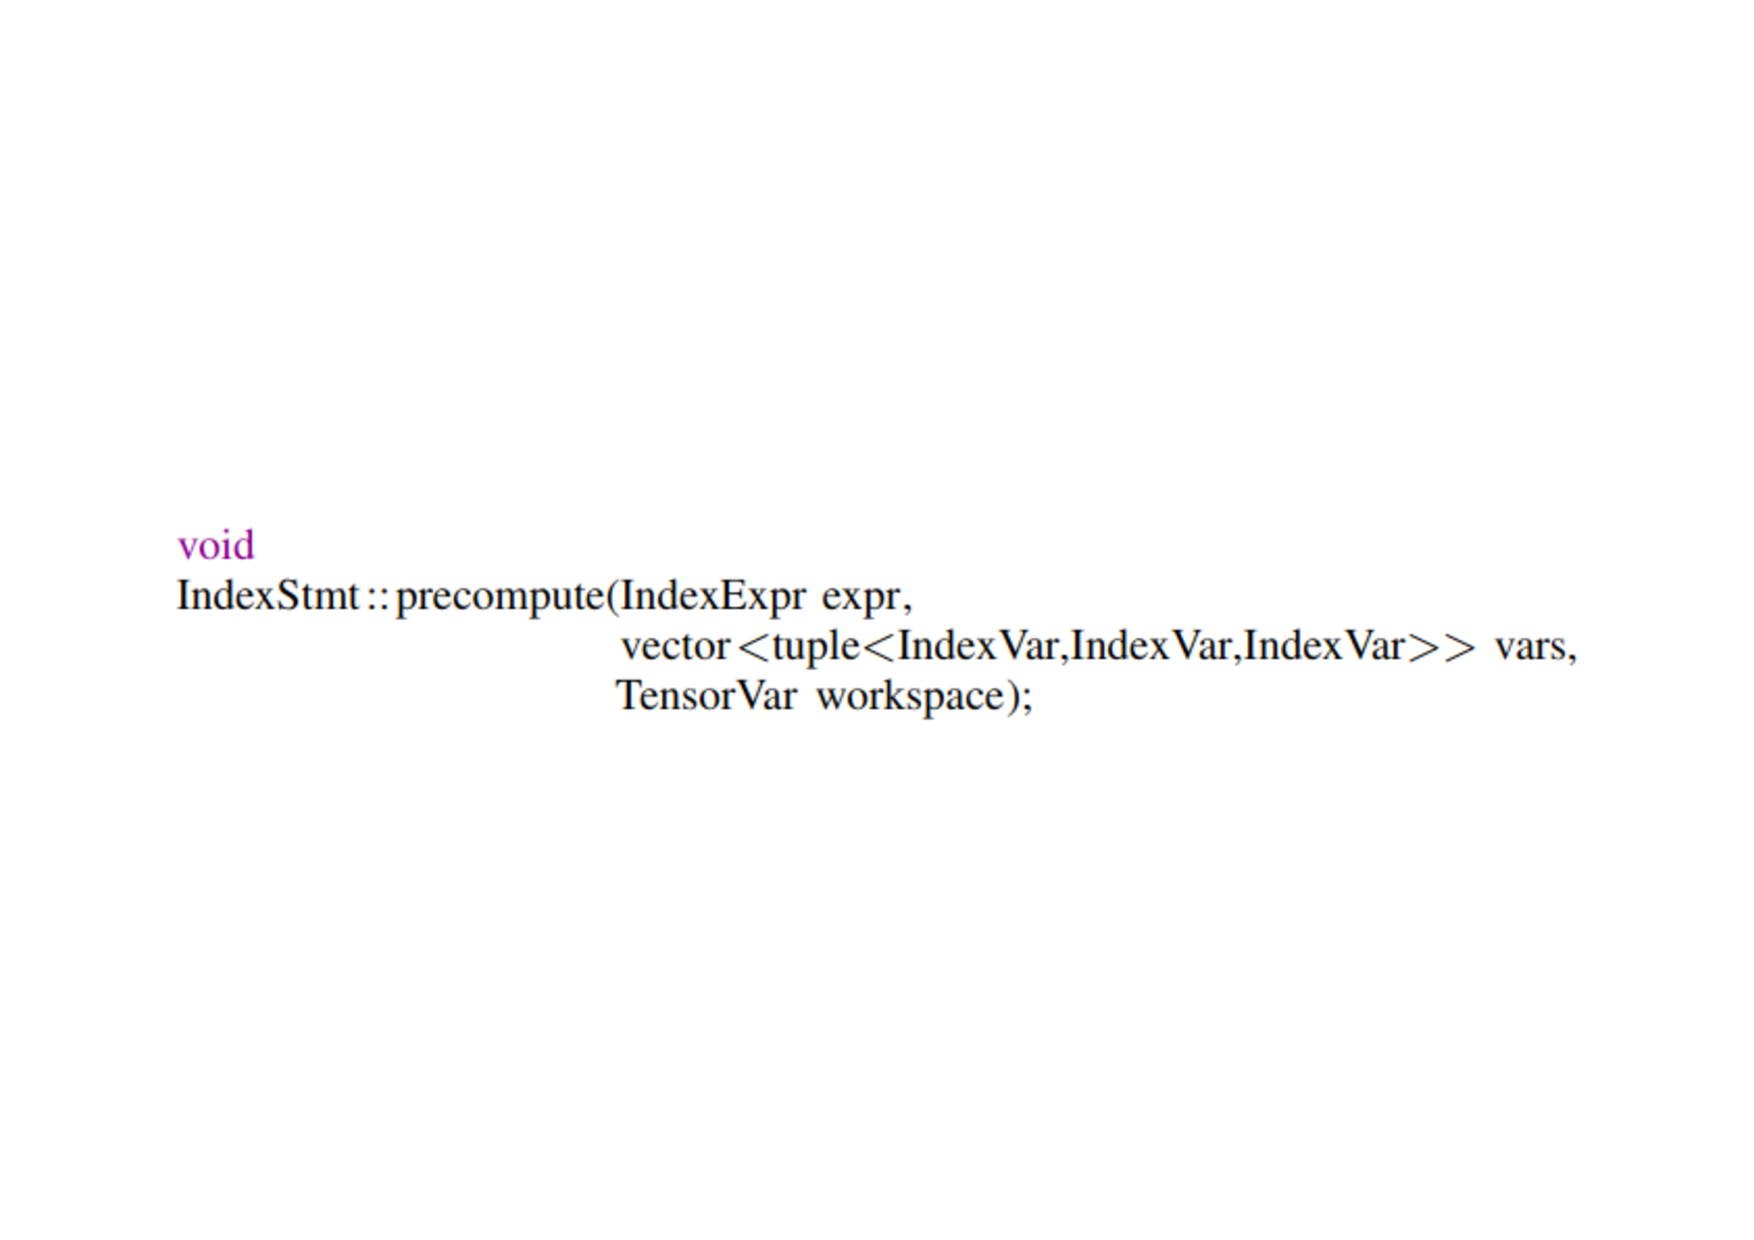
\includegraphics[width=0.35\linewidth]{Precompute-Defination.pdf}}
  \subcaptionbox{预计算调度使用示例\label{fig:c-example}}
    {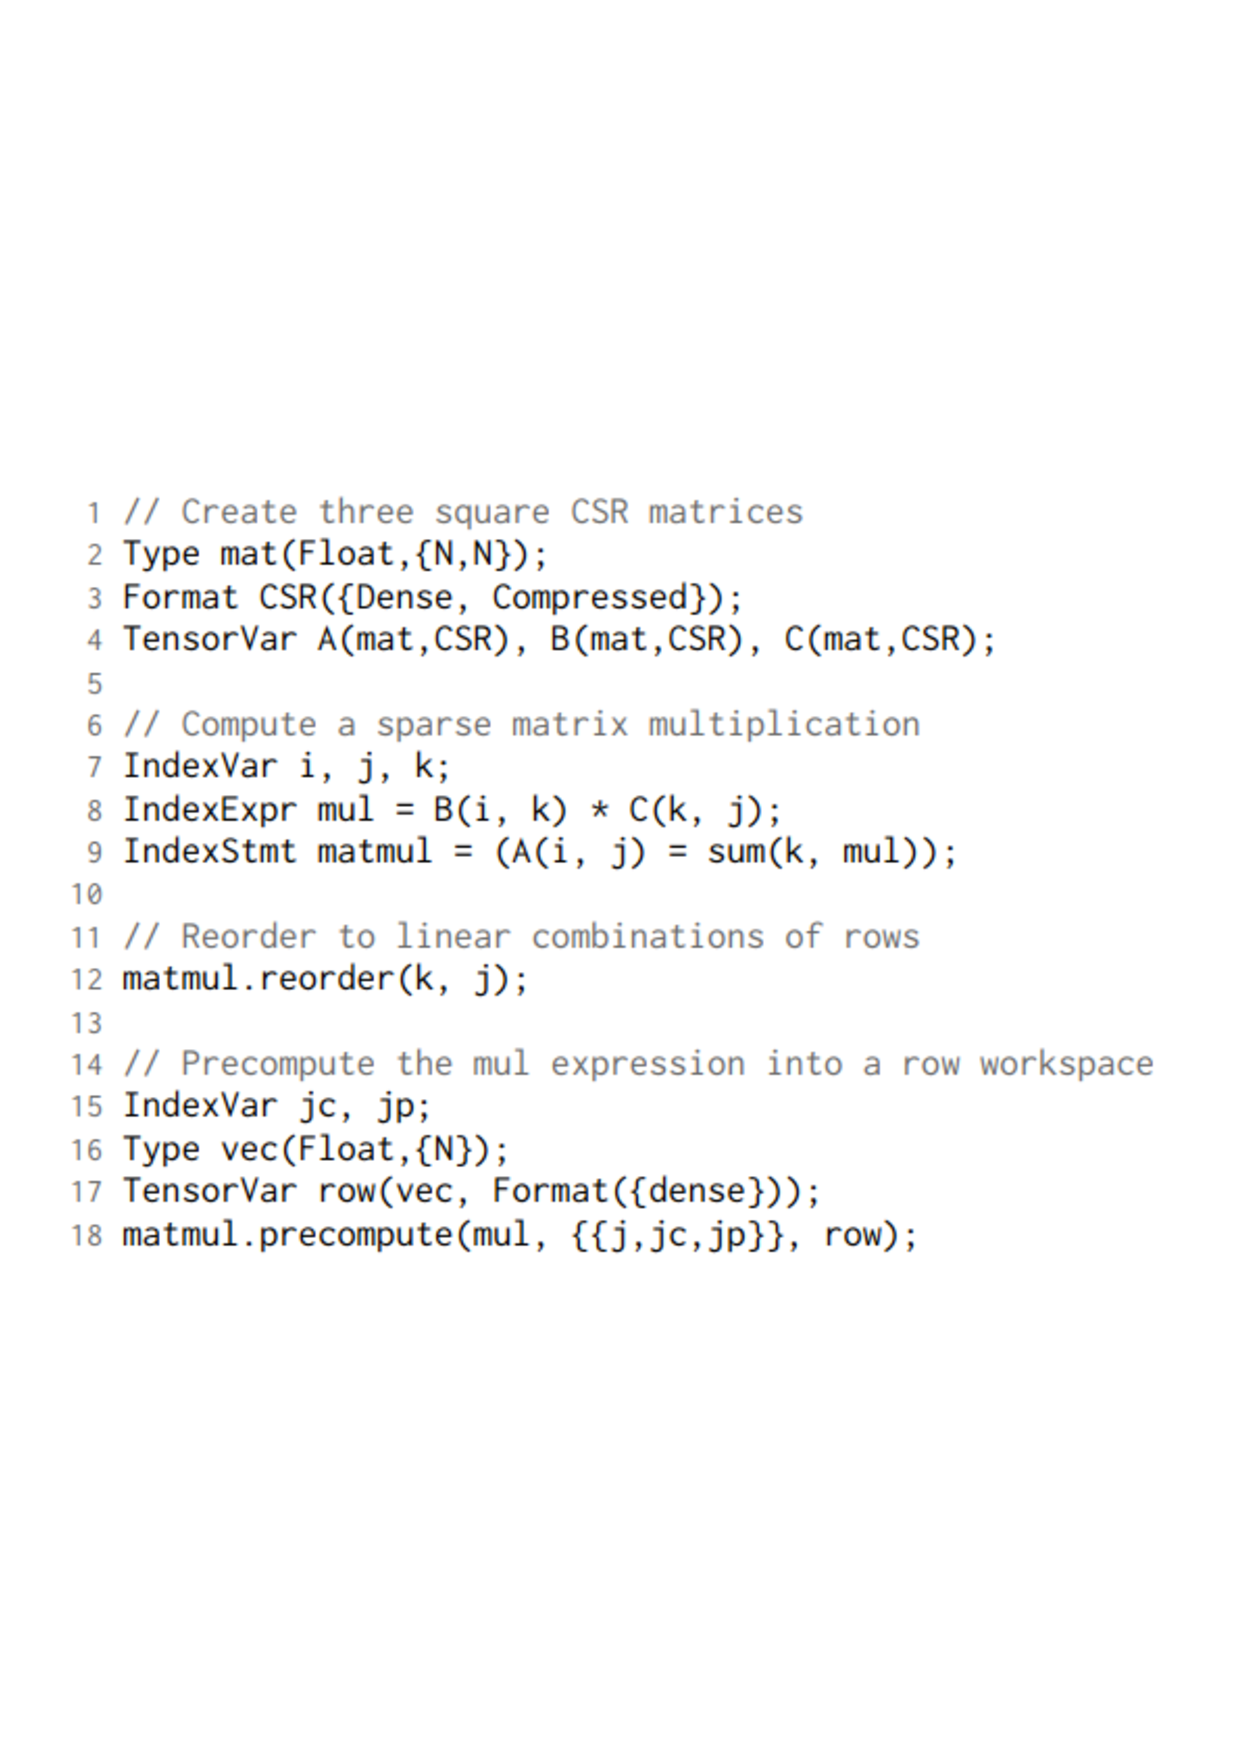
\includegraphics[width=0.35\linewidth]{C++Example.pdf}}
  \caption{预计算调度}
  \label{fig:precomputes}
\end{figure}


我们将预计算方法应用于索引符号语句,并提供要预计算的表达式、要预计算的索引变量以及存储预计算结果的转移空间作为参数。 
expr参数是一个索引表达式,包含在我们调用预计算的索引语句中。vars参数是形式为(old, consumer, producer)的索引变量三元组的向量。 
旧索引变量(old)是我们希望预先计算的变量,它被分成消费者(consumer)和生产者(producer)索引变量。 
生产者变量用于迭代计算转移空间的语句,消费者变量用于迭代使用转移空间的语句。 
最后,转移空间参数是一个张量,用于存储预先计算的结果,其顺序和维度必须足够大以包含所有临时值。
图~\ref{fig:c-example}显示了一个C++示例,它使用重新排序和预计算方法来转换索引表示法语句。
第 2-4 行创建三个具有单精度浮点分量A、B和C的CSR方阵。第7-9行使用索引符号API创建矩阵乘法表达式。
循环的初始顺序是ijk,形成一个内积矩阵乘法算法。 然而,矩阵以CSR行优先矩阵格式存储,因此具有$ C_{kj}$ 访问的ijk循环顺序导致C矩阵在列优先方向上访问。
行优先稀疏矩阵的列优先访问渐近效率低下。 因此,第 12 行对k和j进行重新排序,使对C的访问成为行优先的,并形成行矩阵乘法算法的ikj线性组合。 
然而,重新排序引入了新的效率地下问题。由于 $ A_{ij} $ 中使用的j索引变量现在位于k求和索引变量内,因此代码会将值分散到A中。
但是,A的CSR格式不支持高效随机插入的行优先。因此,第15-18行预先计算并将结果分散到一个稠密的行转移空间中,然后将其复制到A。
稠密转移空间很有用,因为它们支持$ O(1) $随机访问和插入。然而,转移空间可以是任何格式,包括压缩和哈希映射。特别地,哈希映射还支持$ O(1) $随机访问和插入,而无需存储所有零。
此外,转移空间的组件类型可以不同于操作数和结果张量,从而可以使用混合精度算法。例如,图~\ref{fig:c-example}中的行转移空间可以用双精度浮点组件构造,以更高精度地累加值。

\section{具体索引符号}
索引符号是张量代数代码生成器和框架的一种流行输入语言。它描述了张量操作应该做什么,独立于它们的计算方式和访问张量的方式。因此,优化决策不会与算法描述混合。
虽然索引符号是适合张量运算的输入语言,但它不适合作为编译器IR。原因是它没有指定执行顺序或临时张量及其格式。
可以使用几种现有的表示法来完整描述索引表达式的计算方式,例如实现索引表达式的低层次C代码、多面体模型的稀疏扩展或迭代图. 
然而,这些表示自由度过高,无法方便地应用本文中描述的转移空间转换。
我们提出了一种新的张量运算中间语言,称为具体索引符号(Concrete Index Notation)。
具体索引符号使用描述循环顺序、在哪里使用临时变量和临时变量格式的结构来扩展索引符号,但没有关于如何在稀疏数据结构上进行协作的细节。
在编译器软件堆栈中,具体索引表示法是索引表示法和低级命令式IR之间的中间表示。
这种设计的一个好处是我们可以转换具体的索引符号,而不是转换具有间接访问、条件和while循环的稀疏命令式代码。然后在降低具体索引符号时生成稀疏命令式代码。

具体的索引表示法有四种语句类型。赋值(assignment)语句将表达式的结果分配给张量分量,循环(forall)语句在从张量维度推断出的范围内执行语句,暂存(where)语句创建存储子表达式的临时对象,
以及序列(sequence)语句重用临时变量。
为了描述具体的索引符号,我们回到行矩阵乘法示例的线性组合。 我们以ikj顺序用 forall循环表达算法 $\forall_{ikj} A_ij +=B_{ik}C_{kj}$
赋值语句修改单个张量分量的值。它可以是常规赋值(=)或递增赋值(例如,+=,但也允许使用其他运算符)。
在矩阵乘法示例中,递增赋值语句 $ A_{ij} += B_{ik}C_{kj} $ 修改张量分量$ A_{ij} $的值。该语句受到限制,左侧的张量可能不会出现在表达式的右侧,
并且仅使用索引变量访问每个张量。 最后,结果张量被隐式初始化为零。
循环语句通过将索引变量绑定到一组值来表示迭代。循环语句的嵌套描述了索引变量被迭代的顺序。在矩阵乘法示例中,三个forall语句$ \forall_i\forall_k\forall_j $,简写为$\forall_{ikj}$,指定迭代顺序。
暂存语句提前将一个表达式计算结果存储到一个临时的张量变量中。矩阵乘法算法将被方所过的行重复计算和累加到输出矩阵A中。如果A是按照分段压缩格式存储,向行中插入的代价会很高,所以我们可以用一个暂存语句将部分结果累加到一个稠密转移空间中 $\forall_i(\forall_j A_{ij}=w_j) where (\forall_{kj}w_j+=B_{ik}C_{kj})$。
暂存语句引入一个稠密向量$w$来存放右手侧生产者产生的每一行的部分和,然后再复制到左手侧消费者$A$中。
序列语句允许更新张量。假设我们想要把一个CSR格式存储的稀疏矩阵D加到B和C的乘积中。这个操作$ A = D+ BC$ 最好通过服用稠密临时向量$w$实现。与暂存语句不同,一个序列语句中定义在左手侧的张量可以被右手侧张量修改。因此他们可以被用来表达序列的张量写入。


出于多种原因,重新排序具体的索引符号语句很有用。 首先,稀疏张量对它们的访问顺序很敏感。 例如,迭代CSC矩阵的行成本很高,因此我们可以对所有语句重新排序以产生更好的访问模式。
我们可能还希望重新排序以将循环不变的where语句移出内部循环。至关重要的是,我们可能需要重新排序语句,以便我们的转移空间转换的先决条件适用。
当我们重新排序一个具体的索引语句时,我们想知道它会像以前一样做同样的事情。我们可以通过将较大的重新排序操作分解为较小的等价来确保语义等价。
在所有情况下,我们都要求所有被重新排序的语句不包含序列语句。 交换forall语句需要关联属性。如果S是一个用赋值语句修改其张量的语句或用结合运算符的增量语句,
那么 $\forall_i \forall_j S$ 和 $\forall_j \forall_i S$ 在语义上是等价的。 将forall移动到where语句的消费者端类似于循环不变代码移动。
如果$S_2$不使用索引变量j,那么$(\forall_j S_1)where S_2$ 和 $forall_j(S_1 where S_2)$在语义上是等价的。将forall移动到where语句的两侧会改变数据的重用距离。
如果语句 $S_2$ 用赋值语句修改其张量,则$(\forall_j S_1)where (\forall_j S_2)$ 和 $\forall_j(S_1 where S_2)$在语义上是等价的。 
当所有消费者不使用所有生产者的张量时,我们可以重新排列嵌套的where语句。如果$S_1$不使用$S_3$修饰的张量,则$(S_1 where S_2) where S_3$和
$S_1 where (S_2 where S_3)$在语义上是等价的。 如果$S_2$不使用$S_3$修改后的张量,$S_3$也不使用$S_2$修改后的张量,则$(S_1 where S_2) where S_3$和$(S_1 where S_3) where S_2$
在语义上是等价的。

\section{转移空间变换}
转移空间转换使用具体的索引符号where语句在临时转移空间中预先计算张量代数子表达式。它可用于通过以下方式优化稀疏张量代数算子:
\begin{itemize}
 \item 简化合并。同时迭代稀疏张量的代码包含高代价的条件和循环。它可以通过将子表达式预计算到密集的转移空间中来简化。 
 \item 避免高代价的插入。重复累积到稀疏张量的中间是昂贵的。我们可以通过将结果添加到具有快速插入的转移空间(例如密集数组)来提高性能。 
 \item 提升循环不变代码。计算最内层循环中的所有内容会导致冗余计算。 在单独的循环中预先计算子表达式并将结果存储在转移空间中可以提升内部循环的一部分。
\end{itemize} 
转换重写具体索引符号以提取子表达式并单独计算它,将结果存储在临时张量(转移空间)中。 然后可以用主表达式中的临时张量替换子表达式。 
周围的forall语句被下推到子表达式或主表达式中,以避免冗余计算。结果是原始语句一分为二; 一个语句通过转移空间为另一个语句生成值。 
我们可以将转移空间变换视为循环不变代码运动的多维概括,其中我们使用临时张量而不是标量来存储循环不变值。
转移空间变换算法如图~\ref{fig:workspace-transformation}。该转换可以应用于任何二元运算符 $\otimes$ 和 $\oplus$,只要它们都没有副作用并且$\otimes$分布在 $\oplus$ 上。 为了应用转换,我们可能需要首先重新排列语句以匹配 $\forall_J A_K \oplus= E \otimes F$ 的形式。
请注意,如果我们有一个运算符$\odot(x;y) = x$,那么我们可以使用这个运算符来转换将表达式 $A_K \oplus= E$ 和 $A_K = E$ 转换为所需的形式。
执行算法后,我们可以删除 $\odot$ 以简化结果语句。 当 K 包含 I 时,我们还可以将 $A_K \oplus= w_I$ 转换为 $A_K = w_I$,这意味着我们只对 A 的每个元素递增一次。 根据包含 S 的 forall 语句,请求的转换可能无法实现。 
用户需要首先重新排序以删除在 $S'$ 中未使用的索引变量或在 $S^{'}_P$ 和 $S^{'}_C$ 中使用但未包含在 I 中的索引变量的 forall 语句。或者,用户可以向 I 添加索引变量,前提是维度 结果转移空间 w 是 I 中索引变量的数量,维度大小等于这些索引变量的范围。 
我们通过检查每个语句替换来证明转移空间转换是正确的。 第一个替换(拆分语句)是将标量语句转换为等效形式。 for 循环包含接下来的三个替换。 
在我们将 forall 语句移动到 $S^{'}_C$  和 $S^{'}_P$ 的情况下,我们已经检查了 $j \in I$,因此此转换从在分配后立即使用 $w_I$ 的值移动到在 j 循环后使用它们。 我们将 forall 语句移动到 $S^{'}_C$ 的情况等价于循环不变代码运动,
我们将 forall 语句移动到 $S^{'}_P$ 的情况是有效的,因为 $\otimes$ 必须分布在 $\oplus$ 上。在计算两个矩阵的行内积的语句中将转移空间转换应用于 $B_{ij}$ over j 之前和之后的代码。 
在此示例中,转换将同时迭代两行的 j 上的 while 循环替换为独立迭代每一行的 for 循环。 for 循环具有更少的条件,但代价是减少了数据局部性。 
请注意,稀疏代码生成是在编译器堆栈中的具体索引符号下方处理的。
\begin{figure}
  \centering
  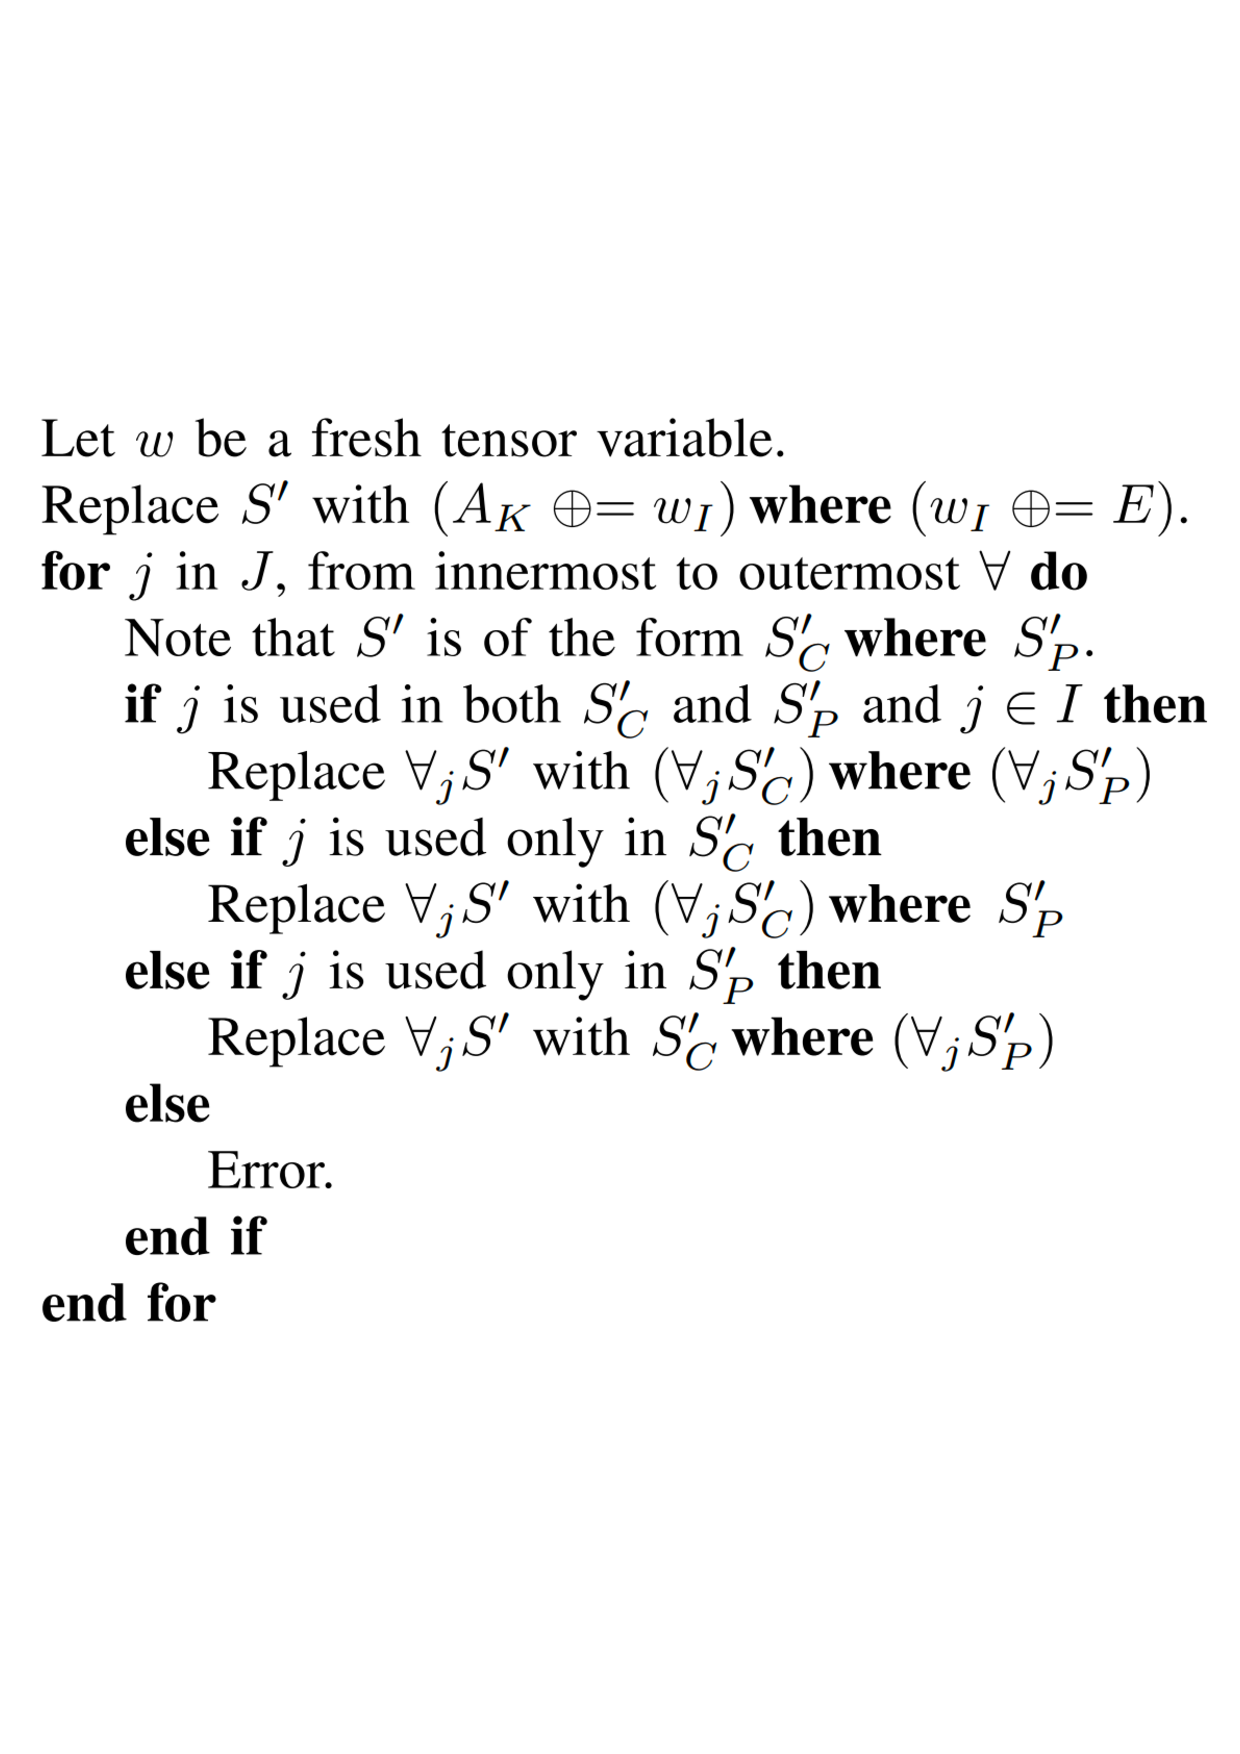
\includegraphics[width=0.5\linewidth]{workspace-algorithm.pdf}
  \caption{转移空间变换算法}
  \label{fig:workspace-transformation}
\end{figure}
三个转移空间变换的目标可以作为简单的启发式条件来描述算子在什么情况下会从转移空间变换中得到性能提升。假设$|$和$i$,且$i\subset I$。我们简单定义三种情况:
\begin{itemize}
  \item 简化合并。形如$(\forall_I A_i \oplus= B_I \otimes C_I \otimes D_I \otimes ...)$的表达式将超过3个稀疏张量$B,C,D,...$合并到稀疏张量$A$,会导致代价较大的合并。
  我们可以通过添加一个稠密转移空间,变换成 $(\forall_I A_i=w_i) where (\forall_I w_i \oplus= B_I \otimes C_I \otimes D_I \otimes ...)$ 
  \item 避免高代价的插入。形如$(\forall_I A_i \oplus= E_I)$的表达式中A是稀疏的,所以会积累到一个稀疏输出。可以通过稠密转移空间来避免稀疏插入,变换成$(\forall_I A_i = w_I) where (\forall_I w_I\oplus= E_I)$
  \item 提升循环不变代码。形如$(\forall_I A_I \oplus= E_I \otimes F_i)$的表达式会冗余计算表达式$F_i$。因此可以变换成$(\forall_I A_I \oplus= E_I \otimes w_i) where (\forall_i w_i = F_i)$
 \end{itemize} 
应用这些启发式条件可能需要先重写表达式,一个表达式不同等价形式的可能会导致有不同性能特征的表达式。

\section{编译}
\subsection{编译算法}
\begin{figure}
  \centering
  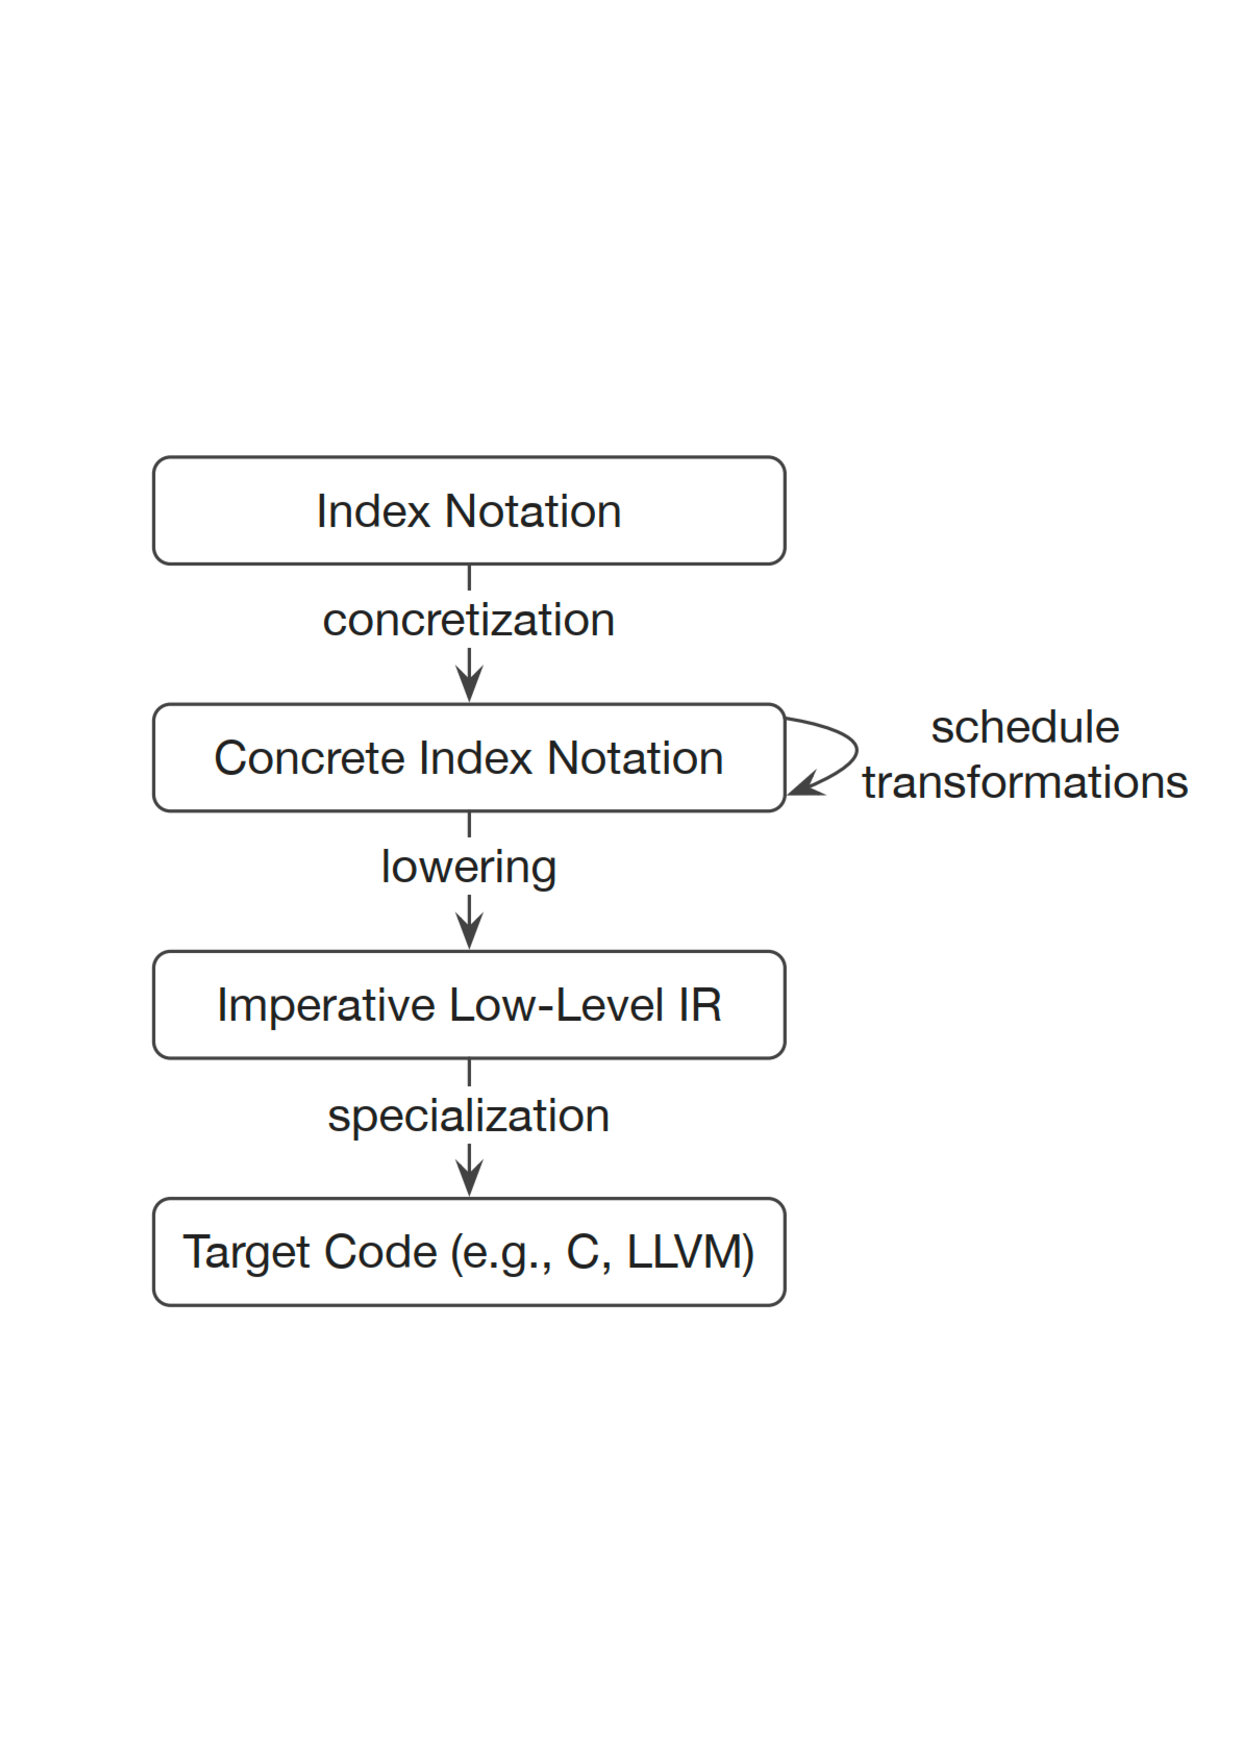
\includegraphics[width=0.5\linewidth]{Compilation-algorithm.pdf}
  \caption{编译变换算法}
  \label{fig:Compilation-transformation}
\end{figure}

\begin{figure}
  \centering
  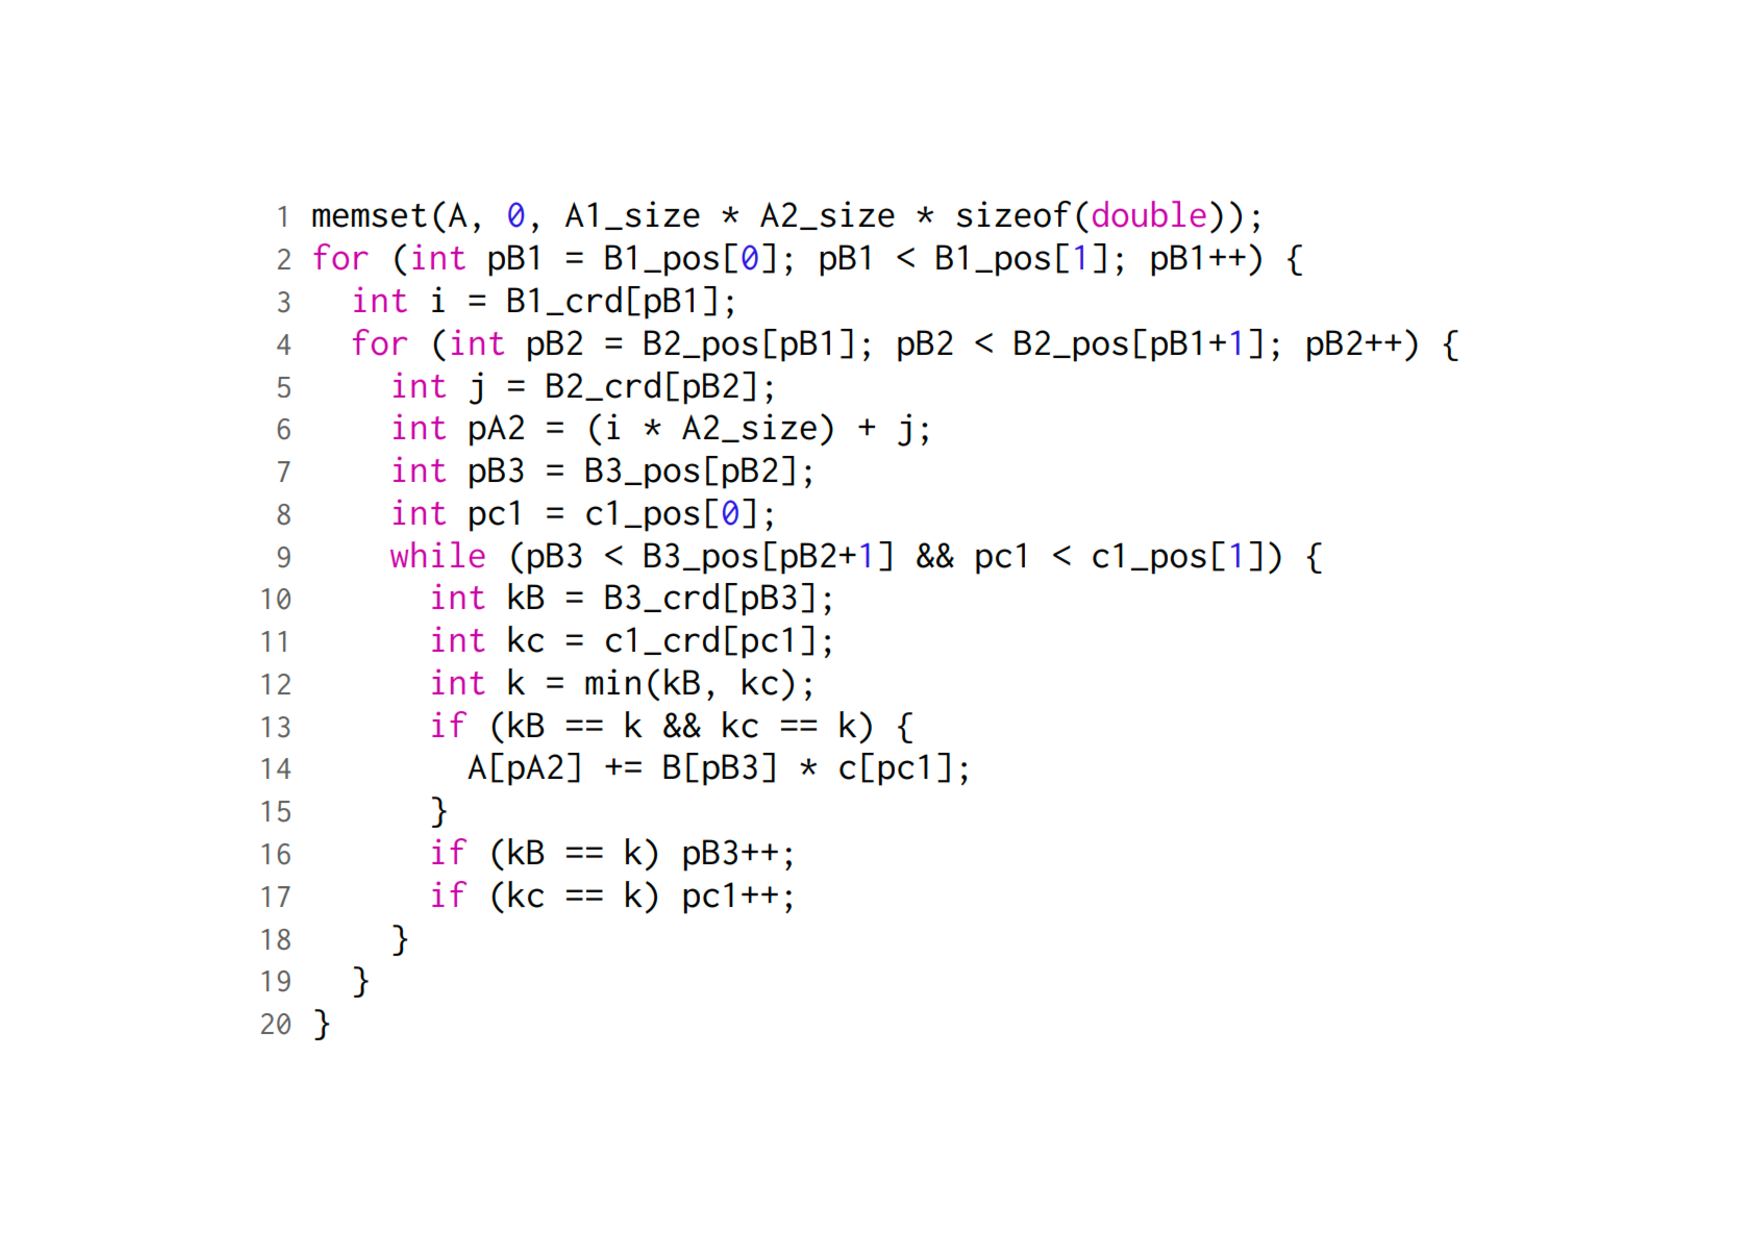
\includegraphics[width=0.5\linewidth]{sparse-vector.pdf}
  \caption{稀疏张量向量乘法代码}
  \label{fig:Sparse-vector}
\end{figure}

本节描述与具体索引符号之间的转换,称为具体化和降级。 图~\ref{fig:Compilation-transformation}显示了编译器工作流程,其中 IR 为方框,IR 转换为箭头。
大多数转换从较高抽象级别的 IR 转换为较低抽象级别的 IR。 然而,转移空间转换转换具体的索引表示法,这些转换是由用户或策略系统以编程方式请求的。 
具体化 IR 转换分两步将索引表示法转换为具体的索引表示法: 在索引表示法表达式中插入用于索引变量的 forall 语句。 
自由索引变量的 forall 语句嵌套在缩减变量的语句之外。 将 reduce 表达式替换为 where 语句,其生产者子语句减少为标量变量。 
结果是有效的具体索引表示法,可以通过转移空间转换进行优化,并进一步降低为低级稀疏命令式代码。 IR 降低将具体的索引符号转换为稀疏的命令式 C 类代码。 
该算法在内部使用我们在之前工作中描述的合并格,但比那里描述的代码生成算法更简单。 增加简单性的原因是它减少了具体的索引符号语句而不是迭代图。 
因此,它不需要在每个递归步骤中推断出哪些子表达式可用于发出。 代码生成算法在具体的索引符号语句上重复出现。 
当它遇到赋值语句时,它会将它们作为标量代码发出。 当遇到 where 语句时,算法会发出生产者端,然后是消费者端。 
最后,当它遇到序列语句时,它发出左侧,然后是右侧。 稀疏代码生成的主要复杂性与 forall 语句的代码生成隔离开来,因为它们必须同时在分层张量数据结构上进行迭代。 
我们建议读者参考我们之前的工作,以获得关于层次协同和迭代图图形符号的更多直觉。 在我们在本文中描述的代码生成方法中,迭代图已被具体的索引符号所取代。 
为了为 forall 语句生成代码,新的代码生成算法遍历 forall 的主体以收集由 forall 的索引变量索引的所有张量模式。 
为 forall 语句生成的代码必须通过协同处理它们的稀疏数据结构来协同处理这些张量模式。 例如,图~\ref{fig:Sparse-vector}显示了用于计算稀疏张量向量乘法的稀疏代码。 
为 i(第 2-3 行)和 j(第 4-5 行)的 forall 语句生成的外部循环仅迭代 B 的稀疏数据结构,因为 i 和 j 仅用于访问 B。
请注意,A 是一个 result 并且不需要迭代,因为根据定义,它的迭代空间与 B 相同。 
然而,为 forall 语句 k(第 9-12 行)生成的内部 while 循环在 B 的最后一个模式和向量 c 的稀疏数据结构上进行迭代。 
由于 B 和 c 相乘,因此 while 循环遍历它们的交集。 如果改为添加它们,则将生成三个 while 循环来共同处理它们的并集。
Forall 语句被降低为命令式代码,使用合并格生成合并代码。 我们建议读者将本说明限制在概述由于使用具体索引符号而导致的算法差异。 
然而,为具体索引符号子语句生成代码的递归调用的处理方式不同。 当在格点递归生成代码时,收集在该点耗尽的数据结构,并重写具体索引符号子语句以通过将它们象征性地设置为零来删除它们。 
因此,我们只对语句中未穷尽的部分进行复现,从而简化了算法。

在计算稀疏结果的代码列表中,到目前为止,我们只展示了计算结果而不组装稀疏索引结构的算子。这让我们可以专注于循环结构,而不会增加转移空间组装的复杂性。
此外,在数值代码中,将组装索引结构(通常称为符号计算)的内核与计算值(数值计算)的内核分开是很常见的。 
我们在之前的工作中概述并在此处修改的代码生成算法可以发出,或者一个同时组装结果索引结构并计算其值的算子。 
当从具体索引符号生成汇编内核时,一个转移空间会产生两个数组,它们一起跟踪转移空间的非零坐标。 
第一个数组(例如,行列表)是已插入到转移空间中的坐标列表,第二个数组(例如,行)是一个布尔数组,用于防止向坐标列表中进行冗余插入。 
图~\ref{fig:assembly-code}显示了稀疏矩阵乘法示例的线性组合的汇编代码。 将转移空间复制到 A 的循环开始于第 32 行。在计算算子中,A 的索引结构已预先组装,
因此代码生成算法会发出循环以迭代 A。然而,在汇编内核中,它会发出代码以迭代转移空间的索引结构。 
此外,汇编内核在第 15-18 行插入转移空间索引(行列表),而不是计算结果,并在第 23 行对索引列表进行排序,以便对 A 的新行进行排序。 
请注意,排序是可选的,只有在必须对结果进行排序时才需要。 最后,汇编内核通过重复加倍在第 26-29 行分配额外的坐标内存。
\begin{figure}
  \centering
  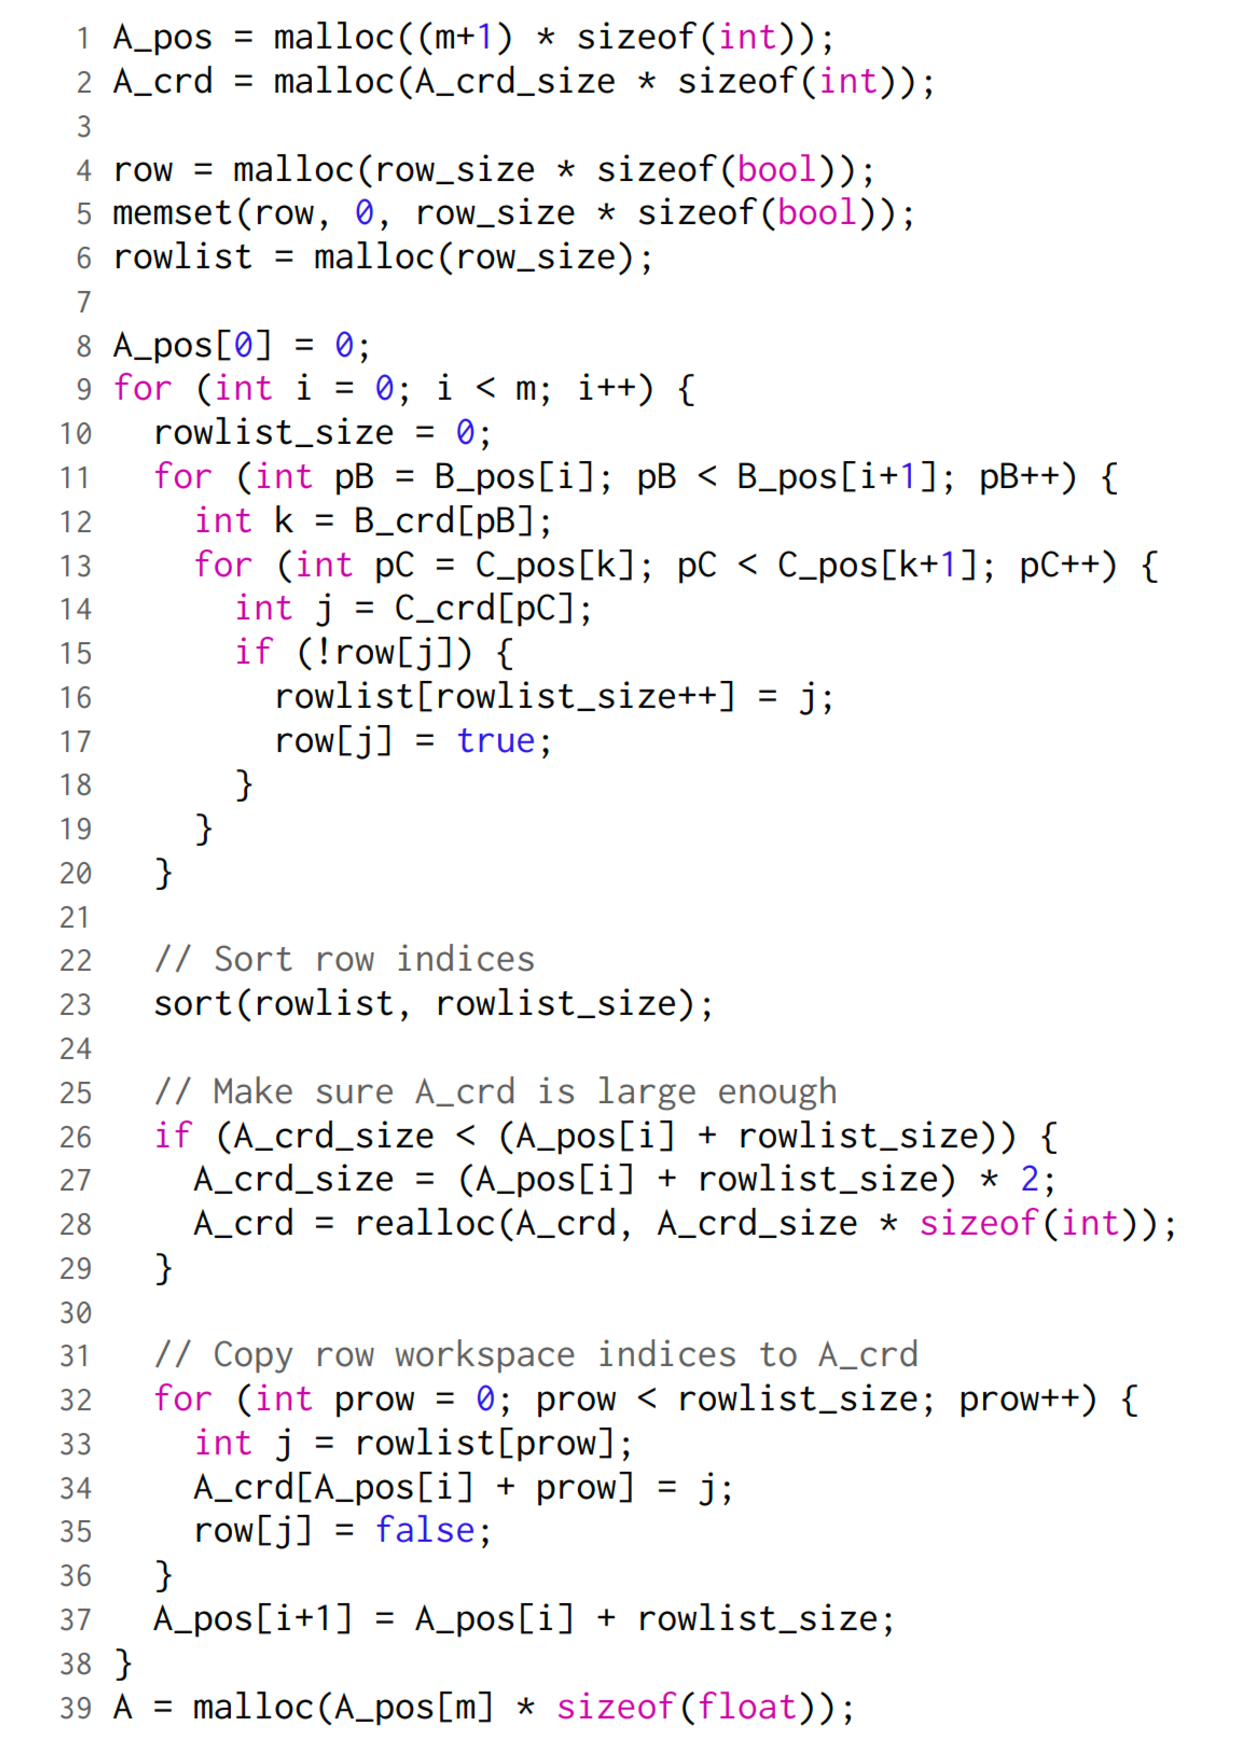
\includegraphics[width=0.5\linewidth]{assembly-code.pdf}
  \caption{汇编代码}
  \label{fig:assembly-code}
\end{figure}

\subsection{案例分析}
矩阵化的张量乘Khatri-Rao积(MTTKRP)在变换最小二乘(ALS)算法中是关键算子。ALS用于计算张量的典范多边体分解(CPD)。
CPD分解是矩阵SVD分解的高维形式,并且在数据分析,机器学习,神经科学,图片分类和压缩以及其他领域中都有广泛应用。
ALS算法和MTTKRP算子可以被用来分解任意维度的张量。对于k维度张量分解的MTTKRP算子由一个k维度张量在不同维度乘k-1个矩阵。例如,四维MTTKRP算子是$A_{ij} = \sum_{klm}B_{iklm}C_{mj}D_{lj}E_{kj}$。
这个部分我们向3维MTTKRP算子应用两次转移空间变换来优化。但是,相同的变换也可以应用在更高维度的算子。MTTKRP算子的第一个转移空间优化基本上等效于SPLATT库中的算法,但是第二个变换让MTTKRP可以写入稀疏输出。
用张量索引符号表达3维MTTKRP算子为
\begin{equation*}
  A_{ij} = \sum_{kl} B_{ikl}C_{lj}D_{kj}
\end{equation*}
MTTKRP最简单的具体索引符号表达形式为
\begin{equation*}
  \forall_{iklj} A_{ij} += B_{ikl}C_{lj}D_{kj}
\end{equation*}
在这个表达形式中forall语句从初始具体形式中变换顺序得到,所以稀疏张量B按照稀疏层级结构的顺序访问。当我们向$B_{ikl}C_{lj}$在j维度应用转移空间变换时得到
\begin{equation*}
  \forall_{ik} (\forall_j A_{ij}+=w_j D_{kj})\, \mathbf{where}\, (\forall_{lj} w_j +=B_{ikl}C_{lj})
\end{equation*}
这个转移空间变换将forall语句中j这一角标变量分裂到where语句两侧的forall语句中。注意l变量没有被消费者中的任何张量利用,因此包含l的语句在消费者中被删除了。这个循环的删除是我们应用转移空间变换的目标
因为这可以导致$w_jD_{kj}$可以在更高的层级计算。这也展示了转移空间变换可以被用来在稀疏代码中提升循环不变的代码。
\begin{figure}
  \centering
  \subcaptionbox{MTTKRP的第一个转移空间变换\label{fig:mttkrp-a}}
    {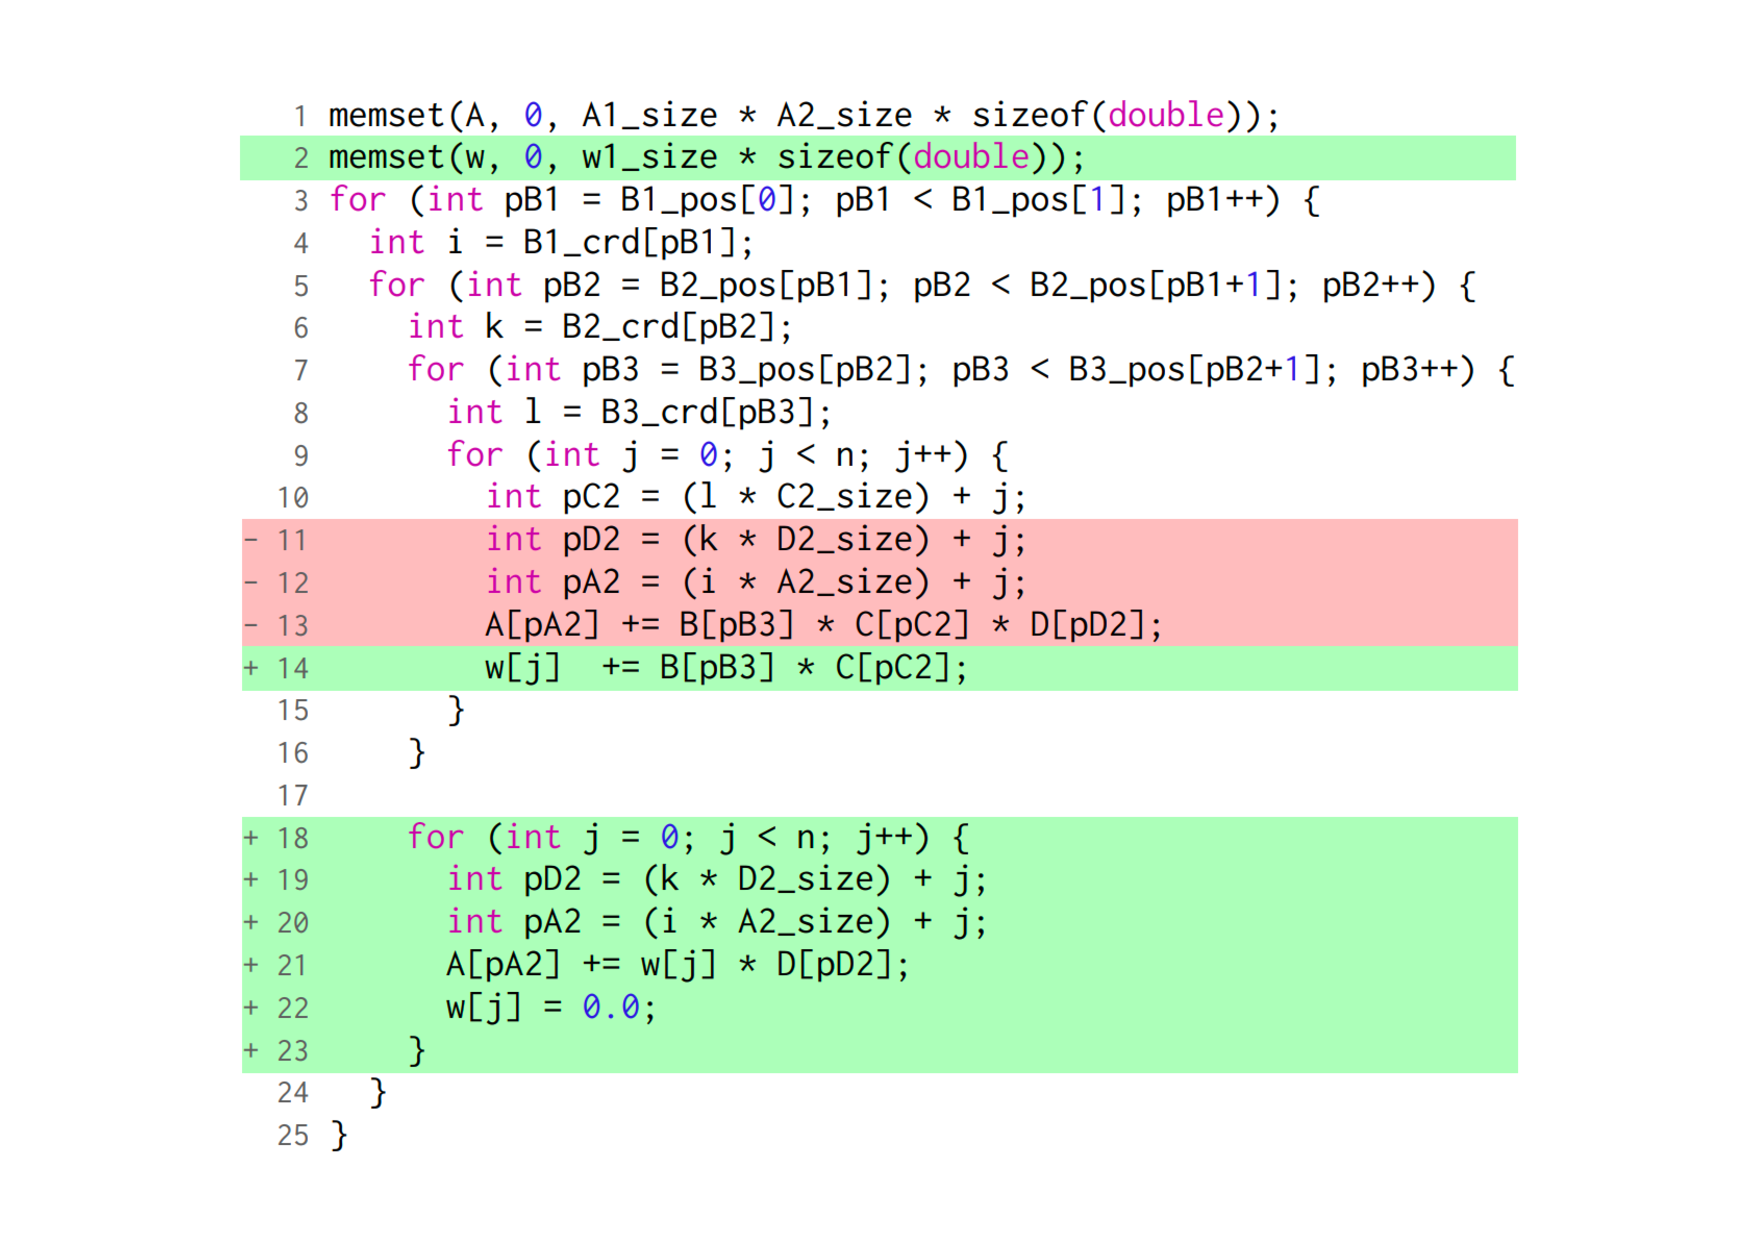
\includegraphics[width=0.35\linewidth]{MTTKRP-1.pdf}}
  \subcaptionbox{MTTKRP的第二个转移空间变换\label{fig:mttkrp-b}}
    {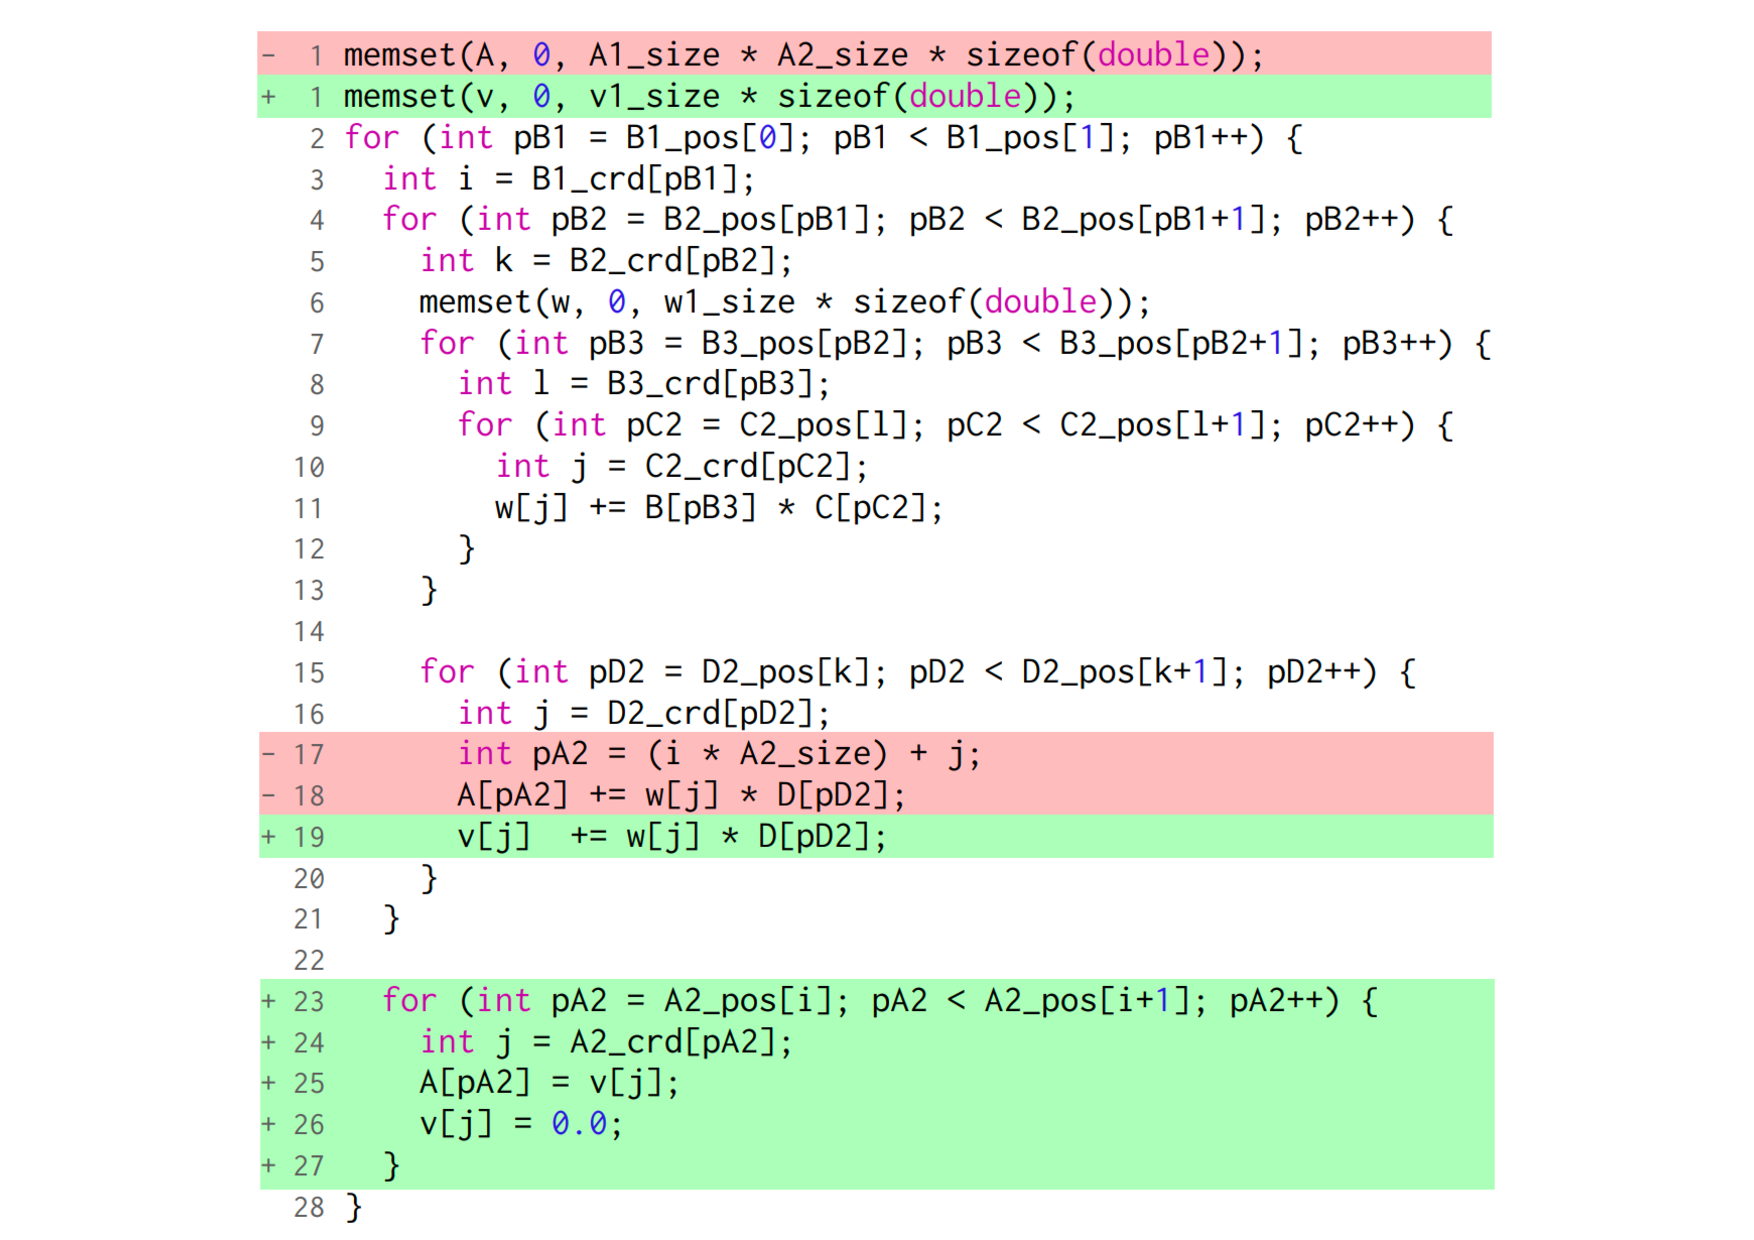
\includegraphics[width=0.35\linewidth]{MTTKRP-2.pdf}}
  \caption{3维MTTKRP}
  \label{fig:mttkrp-code}
\end{figure}
图~\ref{fig:mttkrp-a}中的源代码差异显示了第一个转移空间转换对编译具体索引符号表达式所产生的稀疏代码的影响。 白色背景显示未更改的代码,红色背景显示已删除的代码,绿色背景显示添加的代码。 转换后的具体索引符号生成的代码中,
从第 9 行开始的 j 循环(将 B 与 D 相乘)已从第 7 行开始的 l 循环中移除,从而减少了乘法运算。 代价是转移空间减少了时间局部性,因为写入值和读回它们之间的重用距离。 
实验结果表明,这种特定的转换可以提高两个大型数据集的性能,并降低较小数据集的性能,因此应谨慎应用。
MTTKRP算子会向结果矩阵A中随机写入值。我们可以从累计额的赋值表达式$A_{ij}+=w_j D_{kj}$中观察到这一特征。原因是这个声明在一个或多个forall循环中,并且是一个累加操作。如果A是稀疏的,那么插入就会代价很高。所以,代码性能又会因为应用的转移空间变换而提升。
这次变换为提前在转移空间v中计算$w_jD_{kj}$。得到如下表达式
\begin{equation*}
  \forall_{i} (\forall_j A_{ij}=v_{j})\, \mathbf{where}\, (\forall_k(\forall_j v_j += w_j D_{kj})\mathbf{where}\, (\forall_{lj} w_j +=B_{ikl}C_{lj}))
\end{equation*}
因此,对 A 的赋值不再是递增赋值。 相反,这些值被分散到一个具有随机访问权限的密集转移空间中,然后在计算完一整行结果后复制到结果中。 图~\ref{fig:mttkrp-b}中的源代码差异显示了在转移空间 v 中
生成结果矩阵 A 稀疏和预计算 $w_jD_{kj}$ 对编译代码的影响。转换前的代码(红色)和转换后的代码(绿色)均采用操作数矩阵 C 和 D 是稀疏的,
与图~\ref{fig:mttkrp-a}中的 C 和 D 是密集的相反。 与稀疏矩阵乘法代码一样,转移空间变换后的代码分散到一个密集的转移空间 v 中,
并且在计算出整行后,将转移空间非零值附加到结果中。

\section{性能评估}
在本节中,我们通过将带有转移空间的稀疏内核的性能与用于线性和张量代数的手写最先进的稀疏库的性能进行比较来评估转移空间转换的有效性。
\subsection{实验方法}
所有实验都在双插槽 2.5 GHz Intel Xeon E5-2680v3 机器上运行,该机器具有 12 个内核/24 个线程和每个插槽 30 MB 的 L3 缓存,运行 Ubuntu 14.04.5 LTS。 该机器包含 128 GB 内存并运行内核版本 3.13.0 和 GCC 5.4.0。 对于所有实验,除非另有说明,否则我们确保机器处于空闲状态并报告单线程执行的平均冷缓存性能。
我们通过比较线性代数算子与 Eigen 和 Intel MKL 2018.0 这两个高性能线性代数库的性能来评估我们的方法。 我们还将张量代数内核的性能与用于稀疏张量分解的高性能 SPLATT 库进行了比较。 我们从 SuiteSparse Matrix Collection 和 FROSTT Tensor Collection 中获得了用于实验的真实矩阵和张量。 图~\ref{fig:tensor-info}显示了实验中使用的矩阵和张量的详细信息
\begin{figure}
  \centering
  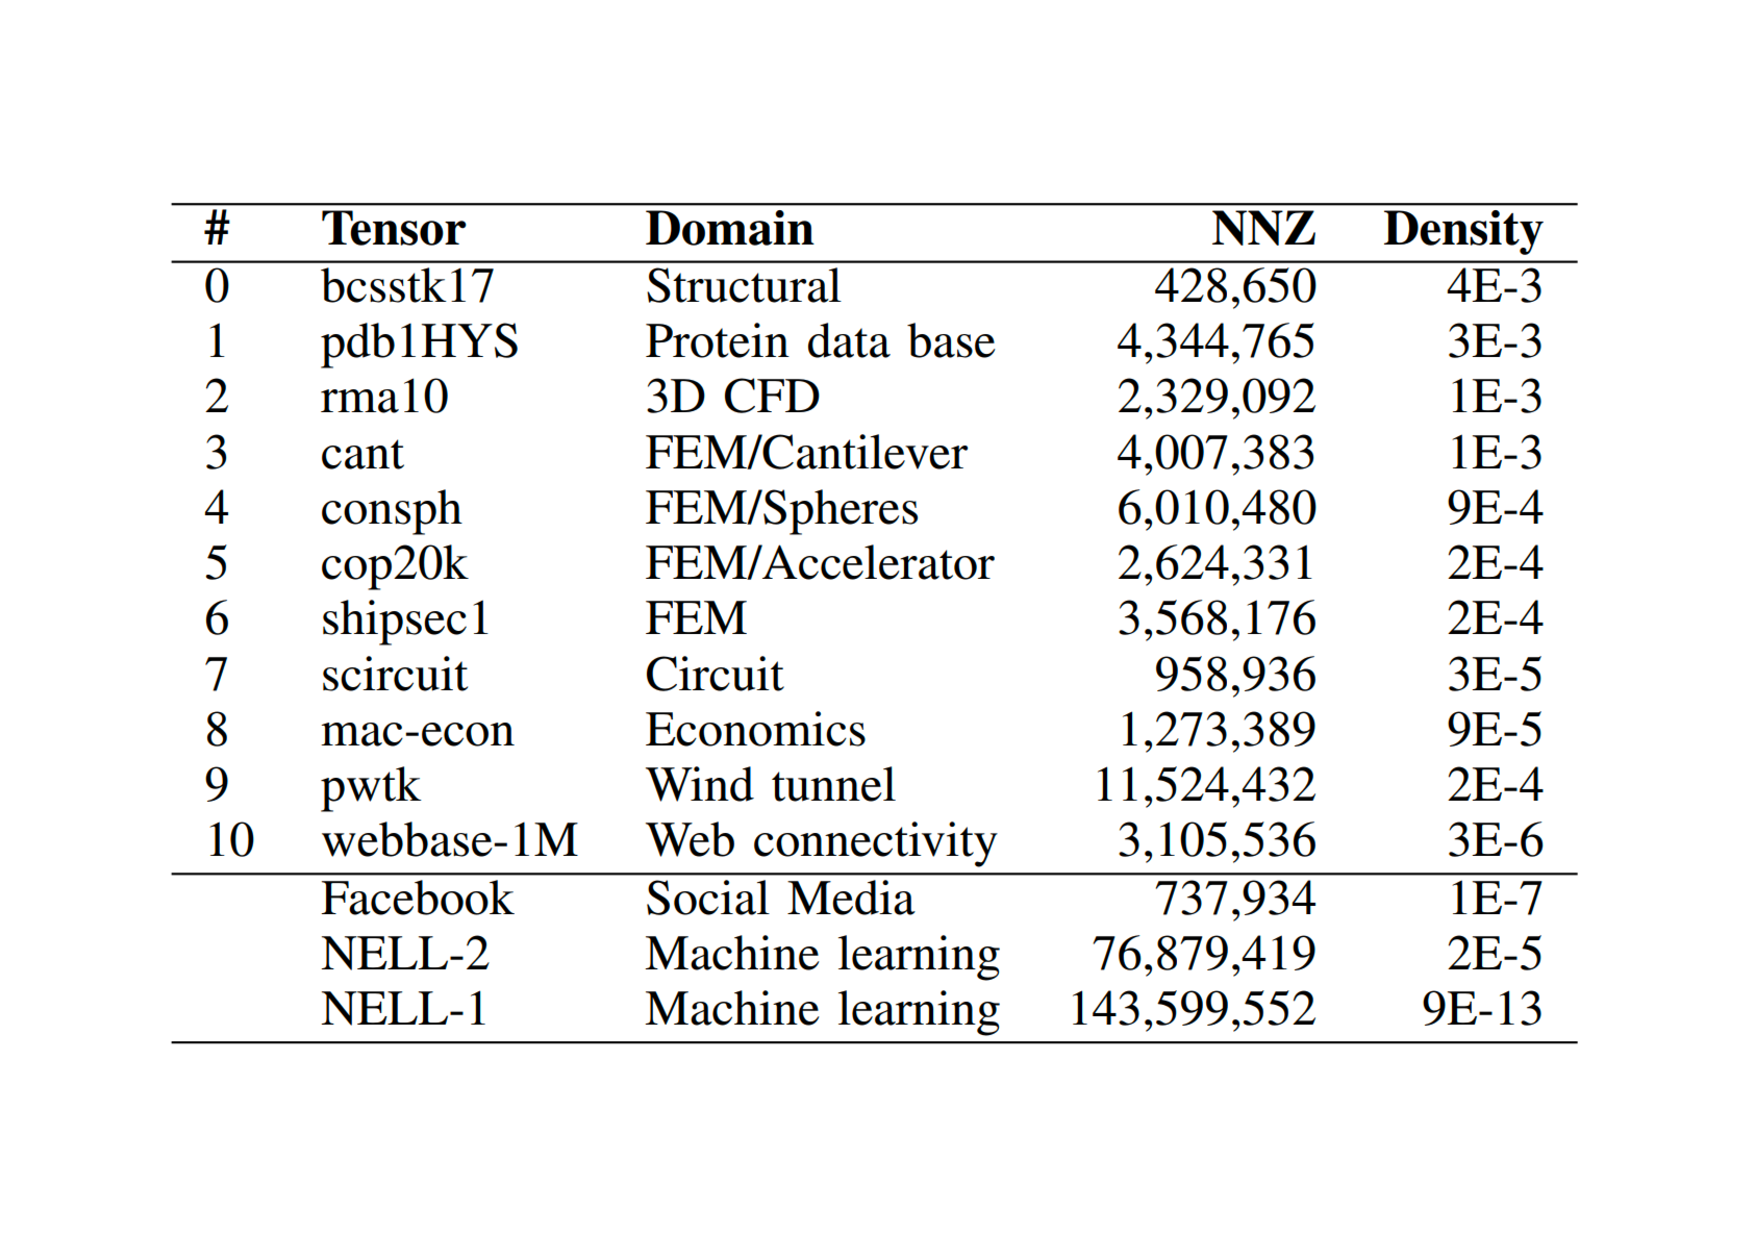
\includegraphics[width=0.5\linewidth]{tensor-info.pdf}
  \caption{实验张量信息}
  \label{fig:tensor-info}
\end{figure}
\subsection{稀疏矩阵乘法}
\begin{figure}
  \centering
  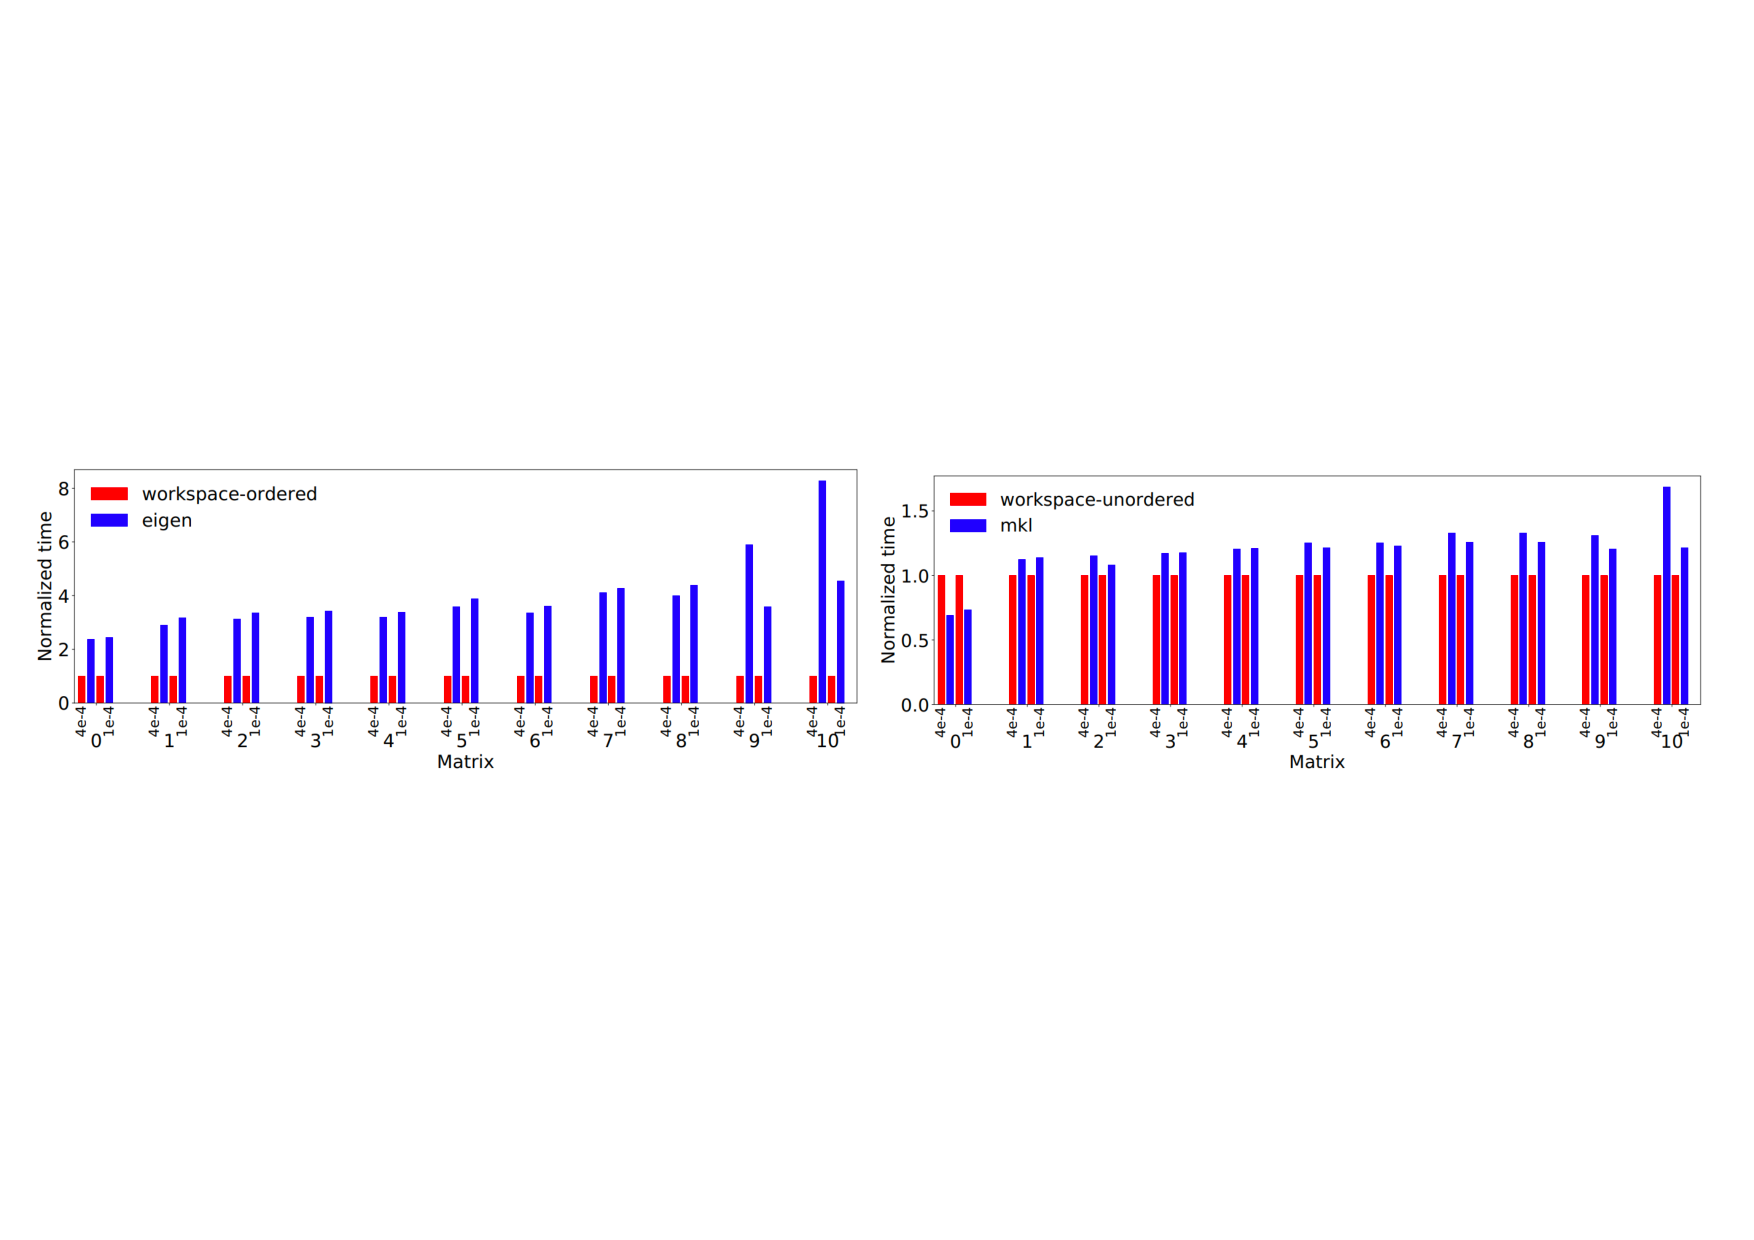
\includegraphics[width=0.5\linewidth]{all-results.pdf}
  \caption{稀疏矩阵乘法实验结果}
  \label{fig:all-results}
\end{figure}
\begin{figure}
  \centering
  \subcaptionbox{3维MTTKRP实验结果\label{fig:mttkrp-results}}
    {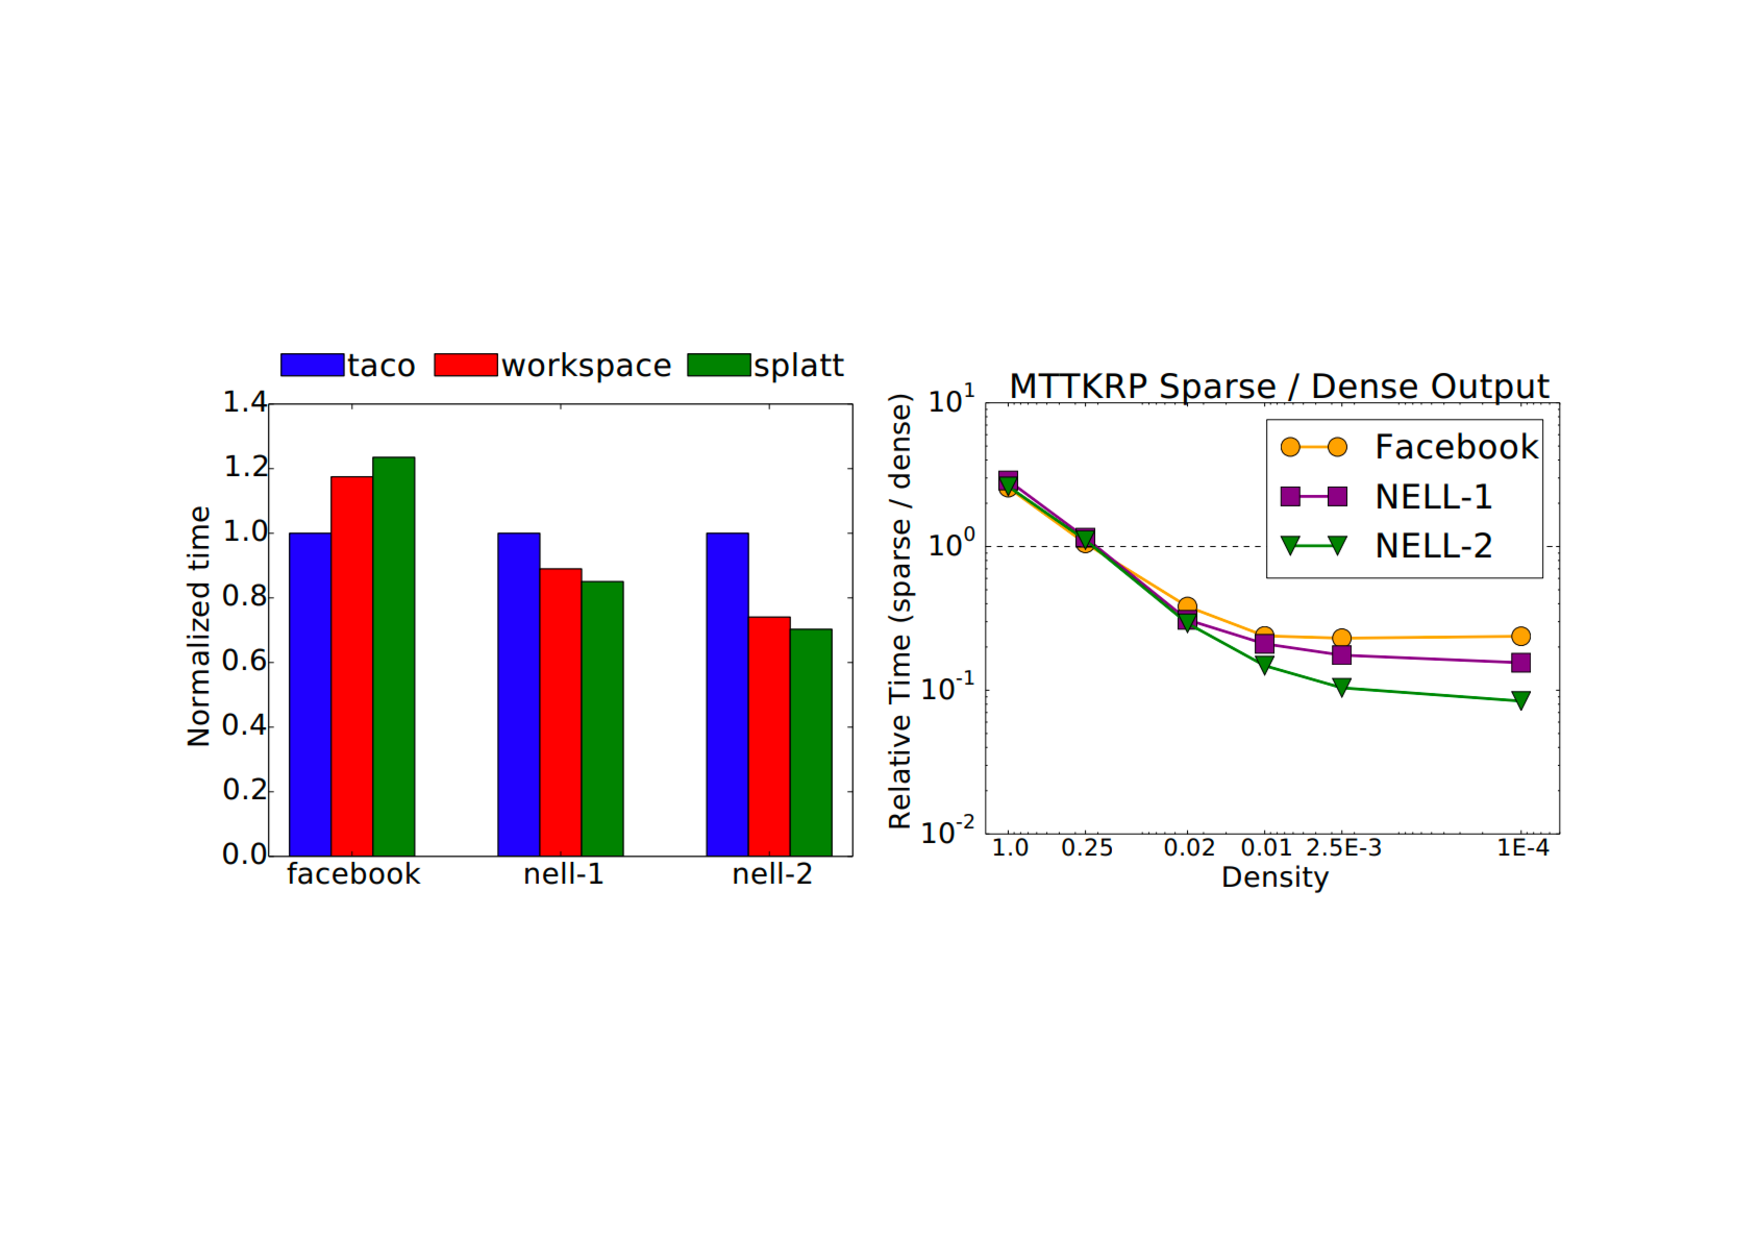
\includegraphics[width=0.35\linewidth]{mttkrp-results.pdf}}
  \subcaptionbox{3维张量加法实验结果\label{fig:spadd-results}}
    {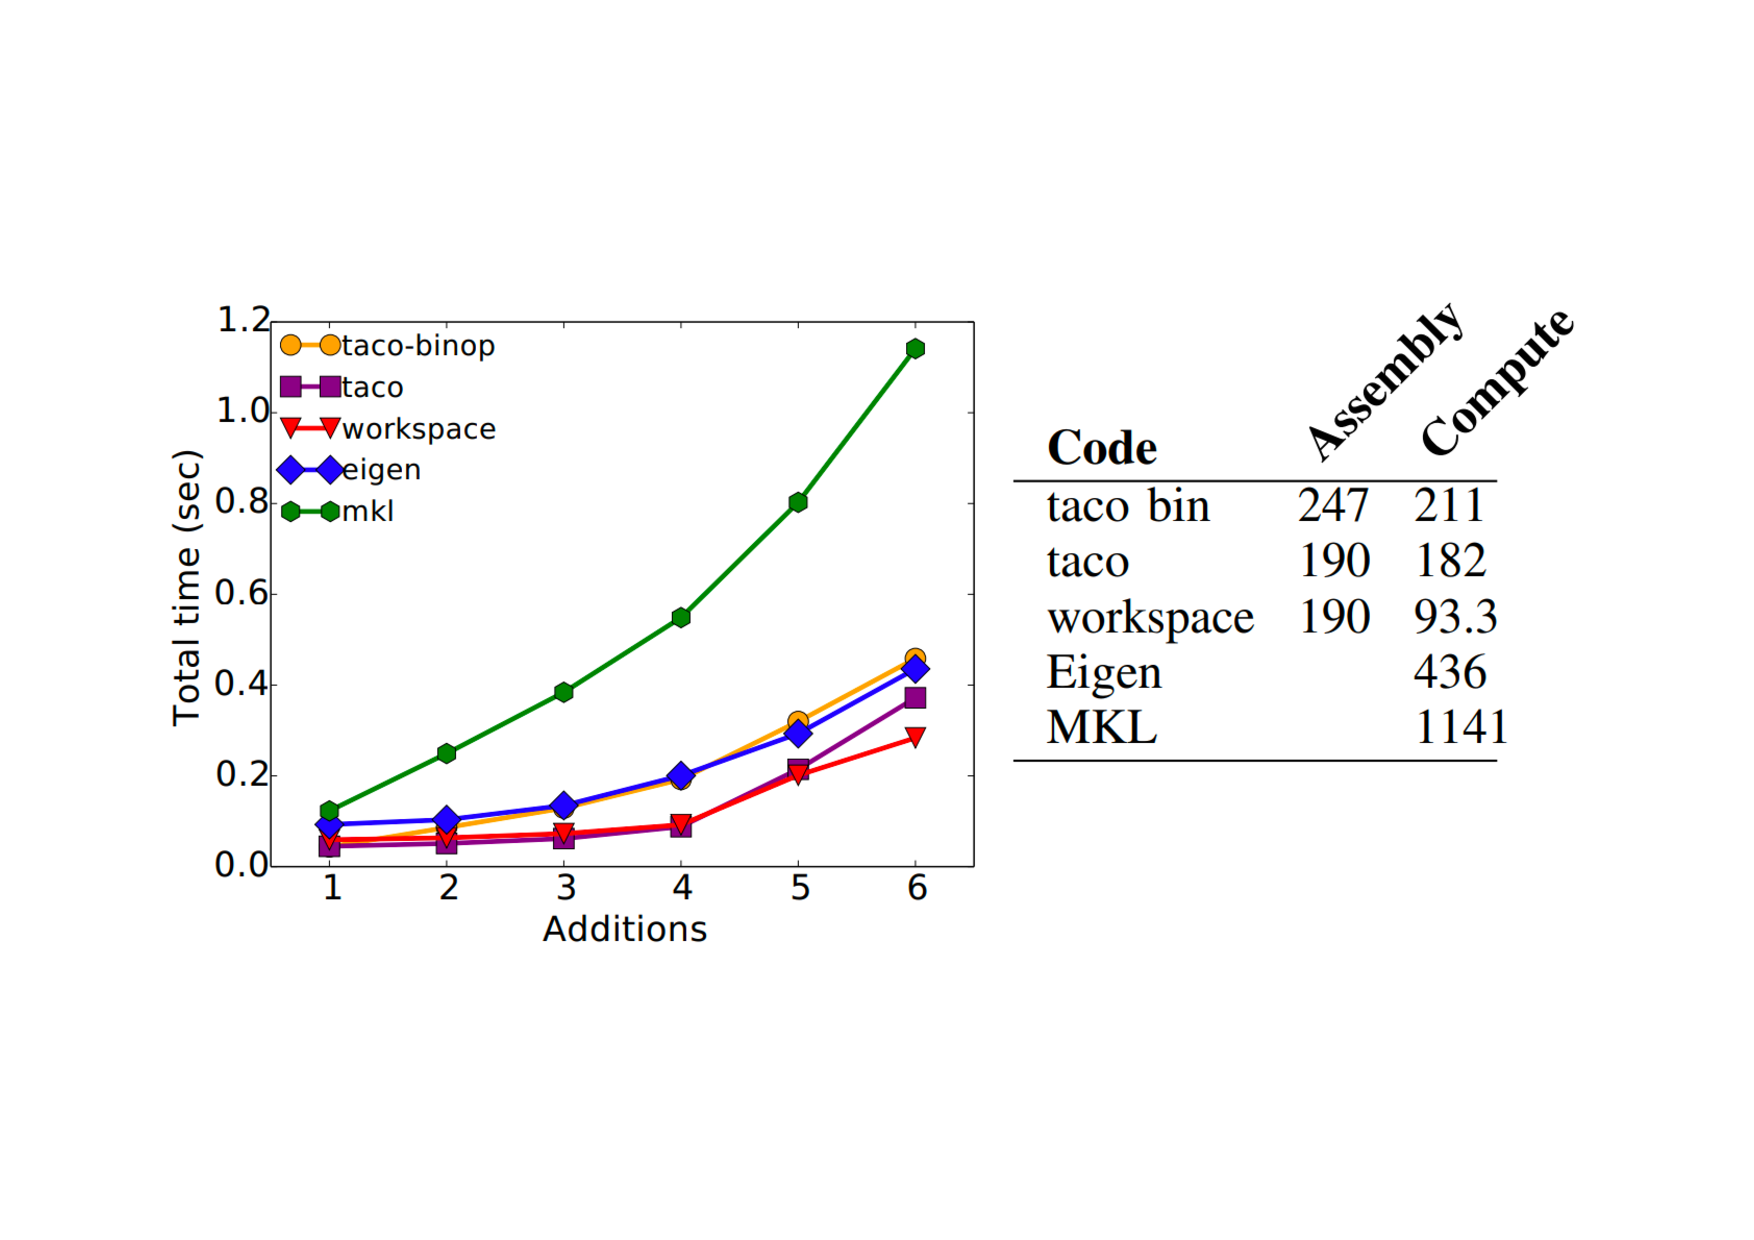
\includegraphics[width=0.35\linewidth]{spadd-results.pdf}}
  \caption{MTTKRP和张量加法实验结果}
  \label{fig:other-results}
\end{figure}

快速稀疏矩阵乘法算法使用转移空间来存储中间值。 我们将生成的转移空间算法与 MKL 和 Eigen 中的实现进行比较。 我们使用两个操作数计算稀疏矩阵乘法:图~\ref{fig:tensor-info}中的真实矩阵和使用特定目标稀疏性和均匀随机非零位置生成的合成矩阵。 Eigen 实现了一种排序算法,该算法对每一行中的列条目进行排序,因此它们是有序的,而 MKL 的 mkl sparse spmm 实现了一种未排序的算法——列条目是未排序的。
因为这两种算法产生不同的成本,我们将其与转移空间变体进行比较每个; 对于排序算法,我们包括排序时间。 在这两种情况下,转移空间算法都将输出矩阵的组装与计算融合在一起。 
请注意,我们之前的实现不会生成稀疏矩阵,因为它不支持插入到稀疏结果中,因此我们在此比较中省略了它。 图~\ref{fig:all-results}显示了图~\ref{fig:tensor-info}中每个矩阵的稀疏矩阵乘法乘以非零密度 1E-4 和 4E-4 的合成矩阵的运行时间,使用我们的转移空间实现。 
平均而言,Eigen 比我们的方法慢,后者生成 Gustavson 矩阵乘法算法的变体,对于两个稀疏度级别分别慢 4 倍和 3.6 倍。 
对于未排序的算法,我们与 MKL 进行比较,发现我们的性能平均快 28\% 和 16\%。 生成的转移空间算法比 MKL 的手动优化实现更快(最多 68\%),只有一种情况除外,后者慢 31\%。

矩阵化张量乘积 Khatri-Rao 积 (MTTKRP) 用于计算数据分析中的张量分解。 三维版本将一个稀疏 3 张量和两个矩阵作为输入,并输出一个矩阵。 图~\ref{fig:mttkrp-results}显示了我们的转移空间算法在三个输入张量上的结果,
与 taco 和手动编码的 SPLATT 库进行了比较。 我们比较并行单套接字实现,使用 numactl 将执行限制在单个套接字。
对于 NELL-1 和 NELL-2 张量,转移空间算法分别优于 taco 中基于合并的算法 12\% 和 35\%,并且与 SPLATT 的手动编码性能相差不到 5\%。 在较小的 Facebook 数据集上,合并算法比我们的实现和 SPLATT 的都快。 
不同的输入在不同的算法下表现更好,这证明了能够生成两个版本的算法的优势。 由于 MTTKRP 是广泛使用的交替最小二乘张量分解算法的最大瓶颈,占计算时间的 69-99\%,我
们预计使用转移空间变换加速 MTTKRP 将为整体张量分解运行时间提供类似的加速。

支持张量和矩阵操作数都是稀疏的MTTKRP也非常有用,如果结果也是稀疏的,则 MTTKRP 可以更快,因为它只需要迭代非零值。 然而,代码很难编写,并且不能由当前版本的 taco 生成。 在本节中,我们评估稀疏 MTTKRP 的转移空间实现。 
因为我们没有实现具有稀疏输出的 MTTKRP 的并行版本,所以我们与两个 MTTKRP 版本的单线程实现进行比较。 哪个版本更快取决于稀疏操作数的密度。图~\ref{fig:mttkrp-results}显示了比较具有稀疏矩阵的 MTTKRP 与具有密集矩阵的
MTTKRP 的计算时间的实验,因为我们改变了随机生成的输入矩阵的密度。 对于每个张量,交叉点大约为 25\% 的非零值,这表明即使输入中只有适度的稀疏性,这
种稀疏算法也可以更快。 在极端情况下,对于我们的三个测试张量,密度为 1E-4 的矩阵操作数可以获得 4.5-11 倍的加速。

为了演示稀疏矩阵加法转移空间的实用性,我们展示了算法随着操作数数量的增加而扩展。 在图~\ref{fig:spadd-results}中,我们将转移空间算法与一次计算一个加法的 taco 进行比较(作为一个库将被实现),
taco 为加法生成一个函数,Intel MKL(使用其检查器-执行器实现)和 Eigen。 我们预先生成 k 个矩阵,目标稀疏度从 [1E-4, 0.01] 范围内随机选择,
并且始终以相同的顺序添加每个库的相同矩阵。 另请注意,x 轴显示加法的数量,它始终比操作数的数量多 1。 这个实验的结果表明了两件事。 
首先,库因一次执行两个操作数的加法而受到阻碍,必须构造和计算多个临时对象,导致性能低于使用代码生成的性能。 即使采用这种方法,taco 
也比英特尔 MKL 平均快 2.8 倍,而 Eigen 和 taco 表现出具有竞争力的性能。 其次,该实验显示了能够生成基于合并和基于转移空间的稀疏矩阵加法实现的价值。 
最多四次添加时,这两个版本具有竞争力,基于合并的代码稍快一些。 但是,随着添加次数的增加,转移空间代码的性能开始优于 taco 实现,
随着添加的操作数越来越多,差距越来越大。 图~\ref{fig:spadd-results}(右)分解了添加 7 个操作数的性能,分离了 tacobased 和转移空间实现的组装时间。 
对于这个实验,我们重用 taco 生成的矩阵汇编代码来构建输出,但使用转移空间进行计算。 大部分时间花在汇编上,这并不奇怪,因为汇编需要内存分配,
而计算只执行逐点工作,没有 MTTKRP 和稀疏矩阵乘法中发现的那种减少。

\section{相关工作}
相关工作分为稠密和稀疏张量代数编译工作、一般循环优化工作、具体索引符号的替代方法以及特定矩阵和张量算子中的手动转移空间转换。 在优化密集矩阵和张量计算方面已经做了很多工作。
研究人员还致力于稀疏矩阵计算的编译和代码生成,包括 Bik 和 Wijshoff、伯努利系统 和 SIPR。 此外,本文基于我们最近关于稀疏张量代数理论和工具的工作,该理论编译稀疏和
稠密张量的张量索引符号,并且我们已经扩展到涵盖更多稀疏张量格式. 然而,这些稀疏编译方法并没有生成带有张量转移空间的稀疏代码来提高性能。 
除了删除多路合并代码和分散到稀疏结果之外,循环嵌套中转移空间转换的一种用途是拆分可能发生在不同循环级别的计算。 这导致操作被提升到更高的循环嵌套。 
循环不变代码运动在编译器中有着悠久的历史,可以追溯到 1957 年的第一个 FORTRAN 编译器。 最近,研究人员发现了利用高级代数知识消除循环中冗余的新机会。 
我们的转移空间转换适用于稀疏张量代数,可以从具有间接访问循环边界和许多条件分支的稀疏代码中删除循环冗余。 
多面体模型旨在优化具有仿射循环边界和仿射数组访问的密集循环嵌套。 然而,稀疏代码具有 while 循环和间接数组访问。
最近的工作将多面体模型扩展到这些情况,使用了编译时和运行时技术的组合。 但是,分层间接数组访问的循环嵌套空间很复杂,编译器很难确定何时可以进行优化。 
例如,Spek 和 Wijshoff以及 Venkat 等人的工作。将稀疏代码转换为密集循环并引入条件以确保仅计算非零条目。 
这样,在将代码转换回对稀疏结构进行操作之前,可以应用传统的密集循环转换(例如平铺)。 
然而,这种技术并没有像转移空间变换那样引入密集的临时张量,而是解决了变换已经存在的稀疏访问的正交问题。 
在生成稀疏代码之前,我们的转移空间变换适用于具体索引符号级别的稀疏张量代数。 这使得在确保生成代码的合法性的同时执行积极的优化转换成为可能。 
具体索引符号的价值在于在张量表达式中指定计算顺序和该顺序内的临时值,同时在语义上排除循环数据依赖性。 最近文献中的两个类似符号是 Tensor Comprehensions (TC) 
和 GLORE 的 LER。 具体索引符号与这些语言之间的第一个区别是操作数可以是稀疏的,并且在引入稀疏索引、条件和 while 循环之前优化了稀疏表达式。 
此外,TC 由一系列索引符号表达式组成,其中循环由索引变量隐含,因此它不能表达内部维度的转移空间(TC 的 where 子句设置索引范围)。 
我们的符号表达排序的方式与 GLORE 的 LER 符号相同,但表达临时计算的方式不同。 首先,我们的符号使用 where 子句来表达包括归约在内的所有临时计算,
而 LER 具有归约表达式。 其次,我们的符号在循环表达式内有标量赋值,而 LER 在循环表达式外有张量赋值。 因此,LER 将临时计算表示为单独的语句,
并且不能在没有以另一种表示法进一步循环融合的情况下在循环嵌套内表示临时计算。 第一次使用密集转移空间进行稀疏矩阵计算是 Gustavson 的稀疏矩阵乘法实现,
我们使用转移空间转换重新创建了它。 用于累积临时值的转移空间在其他工作中称为扩展实累加器,或者称为抽象稀疏累加器数据结构。
Patwary 等人将密集转移空间和分块结合使用来生成快速并行代码。他们还尝试了哈希映射转移空间,但报告说它的使用性能不佳。 
此外,Buluc 等人。 使用分块和转移空间为 CSB 数据结构开发稀疏矩阵向量乘法算法,这些算法对于 $Ax$ 和 $A^T x$的速度同样快。
Im 和 Vuduc等人以 BCSR 稀疏矩阵格式存储常规密集块,并提供多种启发式选择。

\section{总结}
本文介绍了一种将转移空间引入稀疏代码的转换,以消除对稀疏结果的插入,删除条件,并提升循环不变计算。 该转换以新的具体索引符号 IR 表示,用于描述张量索引符号应如何执行。 
该转换实现了具有稀疏结果的新型稀疏张量计算,并提高了其他张量计算的性能,以匹配最先进的手动优化实现。 我们相信转移空间的重要性在未来将会增加,
因为组合新的张量格式将需要转移空间作为粘合剂。 此外,我们相信具体的索引符号可以成长为一种用于通用张量代码转换的语言,包括循环平铺、条带挖掘和拆分。 
结合成熟的调度语言来控制这些具体的索引符号转换,最终的系统会将算法与调度分开。 这将允许最终用户以张量索引表示法指定他们想要的计算,而性能专家、自动调整系统、
机器学习或启发式方法可以指定执行方式的规范。

% 书面翻译的参考文献
\bibliographystyle{unsrtnat}
\bibliography{ref/appendix}

% 书面翻译对应的原文索引
\begin{translation-index}
  \nocite{kjolstad:2019:workspaces}
  \bibliographystyle{unsrtnat}
  \bibliography{ref/appendix}
\end{translation-index}

\end{translation}
  % 本科生:外文资料的书面翻译
%\input{data/appendix}

% 个人简历、在学期间完成的相关学术成果
% 本科生可以附个人简历,也可以不附个人简历
% !TeX root = ../thuthesis-example.tex

\begin{resume}

  \section*{个人简历}

  2000年12月27日出生于黑龙江省大庆市。

  2019年8月考入清华大学电子工程系。


  \section*{在学期间完成的相关学术成果}

  \subsection*{学术论文}

  \begin{achievements}
    \item Zhang, Genghan, Yuetong Zhao, Yanting Tao, Zhongming Yu, Guohao Dai, Sitao Huang, Yuan Wen, Pavlos Petoumenos, and Yu Wang. "Sgap: towards efficient sparse tensor algebra compilation for GPU." CCF Transactions on High Performance Computing (2023): 1-18.
  \end{achievements}


\end{resume}


% 本科生的综合论文训练记录表(扫描版)
% \record{file=scan-record.pdf}

\end{document}
